\documentclass{thesis}

\usepackage{rlipsum} % Only needed for Lorem Ipsum dummy text.
\usepackage{algorithm,algpseudocode}
\usepackage{array}
\usepackage{graphicx, caption, subcaption}

\newenvironment{conditions}
  {\par\vspace{\abovedisplayskip}\noindent\begin{tabular}{>{$}l<{$} @{${}={}$} l}}
  {\end{tabular}\par\vspace{\belowdisplayskip}}

\thesisTitle{An Improved Approach to Manufacturing the Perfect Krabby Patty}
\thesisType{Master Thesis}
\thesisAuthor{Spongebob Squarepants}
\thesisStudentID{123456}
\thesisMonth{August 2015}
\thesisPrimaryReviewer{Prof.\ Dr.\ Jan Bender}
\thesisSecondaryReviewer{Eugene H.\ Krabs}

\begin{document}
\makeFrontMatter

\mainmatter
\chapter{Introduction}
Liquids simulation is one of the most difficult tasks in realistic modeling. Their complexity ranges from overly time-consuming, high-quality standalone animations to real-time low-resolution systems. Fluid animation is used in a wide range of areas e.g. in the entertainment industry, scientific researches, engineering, etc. 

There are two known techniques for modeling fluid phenomena, which have their advantages and disadvantages. Lagrange methods represent a continuous liquid as a collection of discrete particles, and the properties of the liquid mentioned above are carried by these particles. In contrast to Lagrange methods in Eulerian methods, the simulation domain is discretized into mesh grids and the values of physical properties on grid points are determined by solving the governing equations. In addition to position, speed, and acceleration, pressure, density, and viscosity are among the most frequently used fluid attributes.

In recent years, Lagrangian or so-called mesh-free methods have become a competitive alternative to Eulerian (mesh-based) methods due to their inherent mass conservation, the flexibility of simulation in unbounded domains, and ease of implementation.

Additional to Lagrangian simulation, also known as SPH simulation techniques, there is another related field of fluid surface extraction and visualization. Different techniques help to extract the surface from the SPH particle set. These techniques will be described in further sections. However, these techniques require advanced parameters tunning to achieve good surface quality. In most cases smooth surfaces are obtained in terms of degraded performance, thus it is always a trade-off between surface extraction speed and smooth fluid surface construction.

Nevertheless, already existing reconstruction techniques are prone to generating surfaces that look bumpy and rough in the flat areas. In this thesis two surface smoothing methods were implemented, that based on existing surface reconstruction methods perform internal operations on a uniform grid, which is used for surface extraction, to smooth out the extracted surfaces and remove undesired bumps on the fluid surface.

The first method uses general-purpose blur techniques on a 3-dimensional grid to generate smooth surfaces. Although the approach seems pretty easy to incorporate into the surface extraction, additional efforts should be applied to preserve the small and sharp features of the fluid. The main advantage of the method is its efficiency and ease of implementation. However, this method is not always stable and prone to the generation of artifacts in case of inappropriate parametrization.

The second method which is introduced in this thesis is a smoothing filter based on MLS surface approximation. This technique is widely used in the field of surface reconstruction from point clouds, however, in this theses, another approach is described on the application of the MLS filter on the uniform SDF grid, which is used for fluid surface mesh extraction. This method is good in terms of smoothing scalability and much more stable to over-parametrization, however, the main disadvantage of this technique is its performance penalties due to the necessity to solve linear equations and run time-consuming neighborhood detection procedures.
\chapter{Related Work}\label{sec:related-work}

\chapter{Marching cubes}
\chapter{Research framework}
All fluid surface reconstruction methods described in section \ref{sec:related-work} are based on signed scalar field techniques for surface extraction. Given fluid particle displacement, density, and other SPH information these methods are computing scalar signed field (sometimes referred to as signed distance field (SDF)) values for defined 3D grid vertices domain known as Marching cubes domain. After computation of the SDF values on the grid apply the marching cubes algorithm is applied to calculate surface mesh.

Smoothing algorithms, proposed in this thesis are designed in the way that they can be applied to the reconstruction algorithms with the described infrastructure.

In this work the following methods were implemented for surface reconstruction:
\begin{itemize}
  \item \emph{Muller et. al.} described in \cite{Muller}.
  \item \emph{Zhu-Bridson} method described in \cite{ZhuBridson}.
  \item \emph{Solenthaler} method first introduced in \cite{Solenthaler}.
  \item \emph{Onderik et. al.}, proposed in \cite{OnderikEtAl}.
\end{itemize}
All methods use surface extraction computing SDF and extracting the surface mesh using the MC algorithm. The main difference is the way the SDF is defined (see section \ref{sec:related-work}).

\section{Framework architecture}
To simplify further framework development and testing special care was applied to design the class hierarchy. The class diagram is presented in Figure \ref{fig:class-diagam}.

\begin{figure}[H]
	\begin{center}
		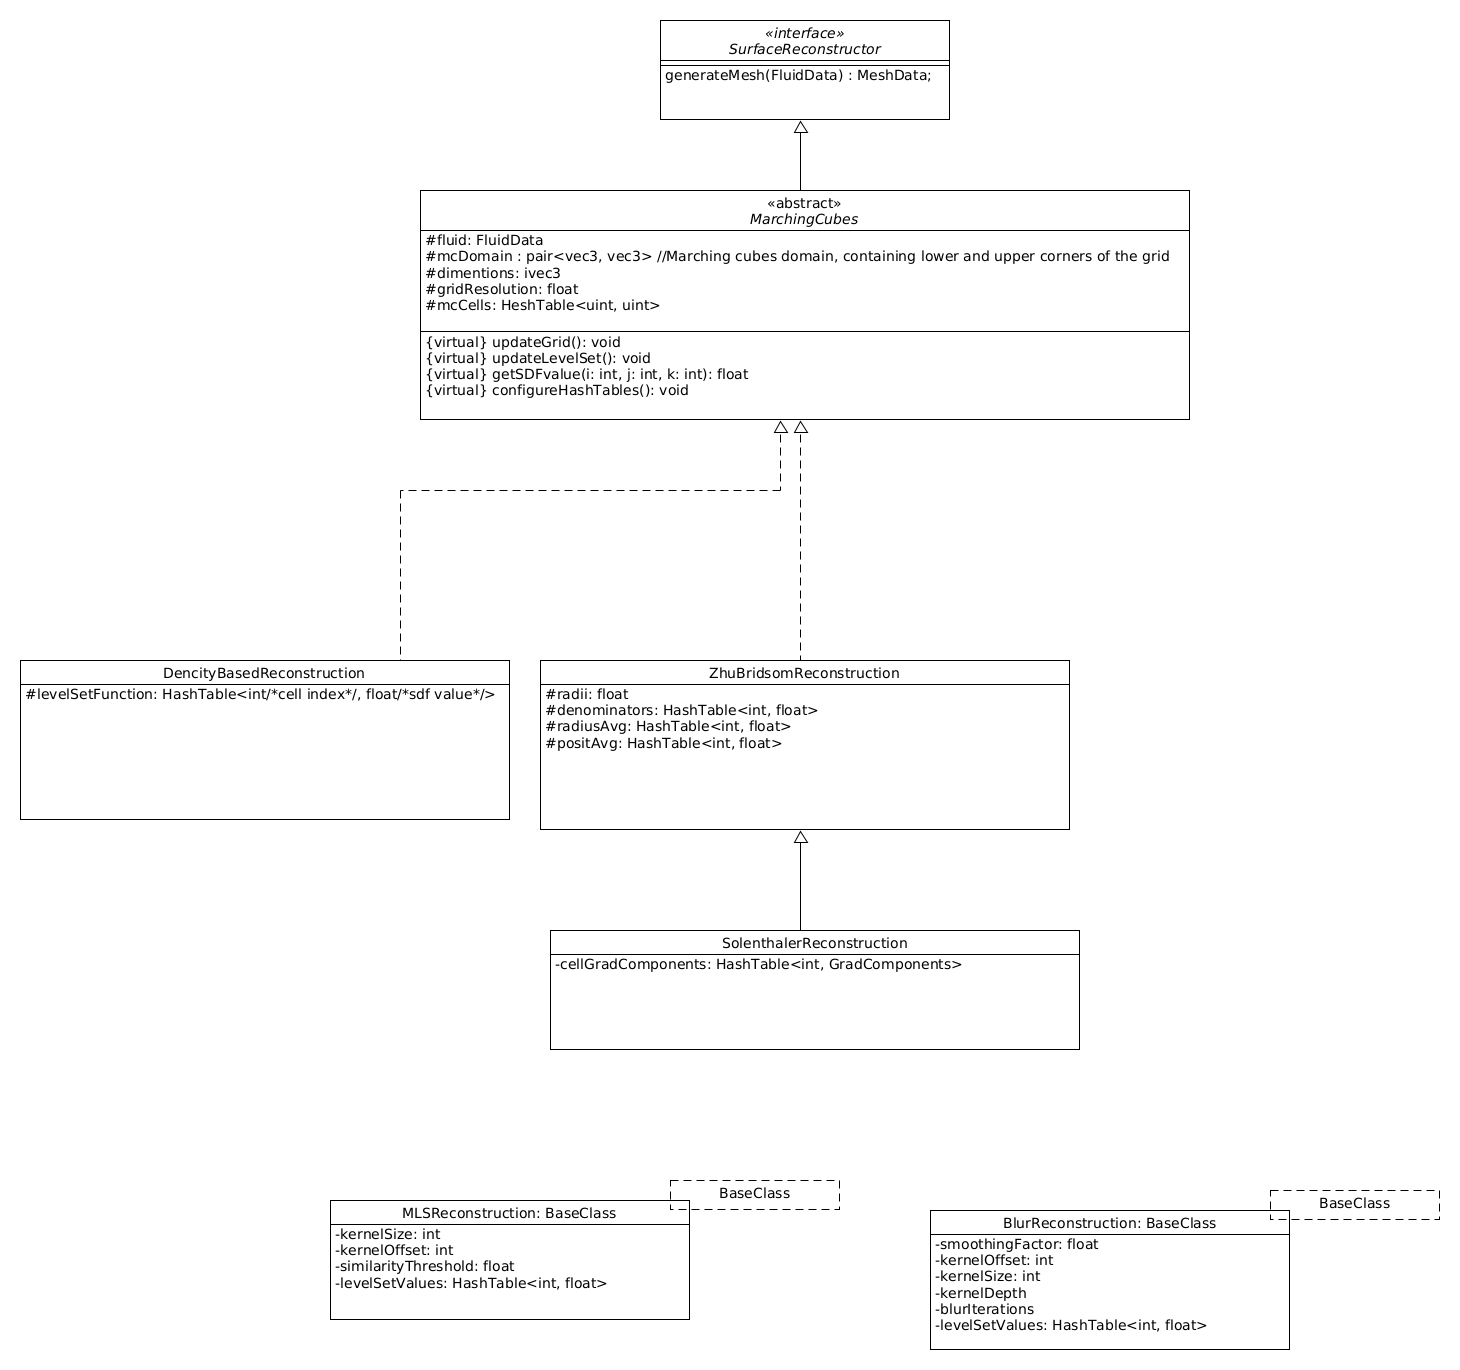
\includegraphics[width=\textwidth]{figures/ClassDiagram.png}
	\end{center}
	\caption{Class diagram, representing inheritance architecture for the surface reconstruction methods}
    \label{fig:class-diagam}
\end{figure}
The base class for all reconstruction methods is \emph{MarchingCubes} class. This class contains common properties for all methods, which exploits the Marching Cubes algorithm. Here \emph{mcDomain} is a pair of two points, representing the domain of marching cubes in 3d space, \emph{dimensions} - is a vector, containing a number of MC grid cells in X, Y, and Z directions, \emph{gridResolution} - the size of each cell (all cells are assumed to be of a uniform size where $width=length=height$), \emph{mcCells} - is a hash table which contains key-value pairs of cell index and a number of SPH fluid particles within its support radius. Each MC cell vertex has its unique integer index, which can be transformed from its position in 3d space. The transformations are extensively explained in \cite{Akinchi}. 

The \emph{MarchingCubes} class has 4 virtual methods, which should be reimplemented inside each subclass:
\begin{itemize}
	\item \emph{computeSurfaceParticles()} - computes color field and detects SPH particles that are resided near the fluid surface.
	\item \emph{configureHashTables()} - inside this method every concrete method performs initial configuration of hash tables, which are used to store SDF.
	\item \emph{updateGrid()} - computes the MC greed domain where calculation of SDF will be performed.
	\item \emph{updateLevelSet()} - calculates SDF values for each MC grid vertex. All smoothing algorithms described here are incorporated in this function and are applied on top of the SDF calculated by underlying method 
\end{itemize}
\emph{MarchingCubes} class re-implements interface method \emph{generateMesh()} composing previously defined functions (see Algorithm \ref{alg:generateMesh}).

\begin{algorithm}
	\scriptsize
	\caption{General overview of the algorithm applied inside each concretisation of MarchingCubes class}
	\label{alg:generateMesh}
	\begin{algorithmic}
		\State $computeSurfaceParticles()$
		\State $configureHashTables()$
		\State $updateGrid()$
		\State $updateLevelSet()$
		\State $mesh \gets computeMesh()$ 
		\State $return\ mesh$
	\end{algorithmic}
\end{algorithm}

\section{Adaptive hash tables for Marching Cubes grid}

As presented in \cite{Akinchi} the computation time for extracting smooth surfaces is mainly influenced by the resolution of the Marching Cubes grid and the smoothing radius R. Achieving high-quality surfaces is possible at the expense of performance. One of the main causes of this issue is computing the scalar field over the volume of the fluid instead of concentrating on the surface area. Thus for performance and memory optimization reasons we decided to apply suggestions, proposed in \cite{Akinchi}.

The first step is to determine the MC grid domain, on which all computation operations will be performed. To perform fluid surface reconstruction it is enough to compute SDF for MC grid cells that are near the fluid surface. To compute these cells next steps are applied:
\begin{itemize}
		\item Compute SPH fluid particles, that are in the nearest neighborhood to the surface of the fluid. To determine surface particles in a preprocessing step, the smoothed color field method \cite{ColorField} is employed.  The smoothed color field value of a particle at position x is computed using Equation \ref{eq:ColorField}.
		\item For each determined particle compute MC grid vertices, that are within the support radius R from each SPH particle, computed in the previous step.
		\item To avoid double layering problem explained in the \cite{Akinchi} additional pass through all SPH particles applied. In this pass for each SPH particle, neighboring MC vertices are queried. If there exists at least one MC grid cell that was identified as a near-surface vertex, the particle is accepted for further processing, otherwise, it is discarded (only for a current frame of the surface reconstruction phase. Modifications are not propagated to the SPH simulation or other reconstruction frames).
\end{itemize}

\begin{equation} \label{eq:ColorField}
	cf_i = \sum_{j\in SPHNeighbors_i}{m_j \cdot \dfrac{W_{ij}}{\rho_j}}
\end{equation}
Where:
\begin{conditions}
	SPHNeighbors_i & set of neighbor fluid particles for particle i\\
	W_{ij} & kernel function\\
	\rho_j & density of particle j\\
\end{conditions}
Detailed instructions sequence described in Algorithm \ref{alg:MC_grid_domain_computation}.
\begin{algorithm}
	\scriptsize
	\caption{Compute MC grid vertices and SPH particles that are going to be processed during computation of the SDF.}
	\label{alg:MC_grid_domain_computation}
	\begin{algorithmic}
		\ForAll{ $particle \in ParticleSet$}
			\State Compute ColorField using Equation \ref{eq:ColorField}
			\If{$ColorField \in ThresholdRange$}
				\State $SurfaceParticleSet \gets SurfaceParticleSet \cup particle$
			\EndIf
		\EndFor

		\ForAll{$particle \in SurfaceParticleSet$}
			\State Compute $Neighbors_i$ of MC vertices within R from  $particle$
			\State $MCGridSurfaceCells \gets MCGridSurfaceCells \cup Neighbors_i$
		\EndFor

		\ForAll{$particle \in ParticleSet$}
			\State Compute $Neighbors_i$ from MCGridSurfaceCells within R from  $particle$
			\If{$Neighbors_i \neq \emptyset$}
				\State $SurfaceParticleSet \gets SurfaceParticleSet \cup particle$
			\EndIf
		\EndFor

		\State $return\ MCGridSurfaceCells, SurfaceParticleSet$
	\end{algorithmic}
\end{algorithm}

As a result the framework is able to perform surface extraction on large scale with up to 13 million SPH particles (see sections \ref{sec:related-work}, \ref{sec:mls} and \ref{sec:blur})

\chapter{Blur level set}
During the reconstruction of the surface all methods in one form or another (depending on the level set computation approach) are using particle displacement information. In the SPH based fluid simulation frameworks fluid particle displacement usually are formed irregularly, thus small insufficient gaps or buimbs can be formed during the surface reconstruction phase, which are usually treated as undesirable low-frequency noise. The comparison of the surface reconstruction based on a regular and irregular displacement of the particles is in Figure \ref{fig:rec_vs_displacement}.
\begin{figure}[H]
	\begin{center}
		\begin{subfigure}[b]{0.6\textwidth}
			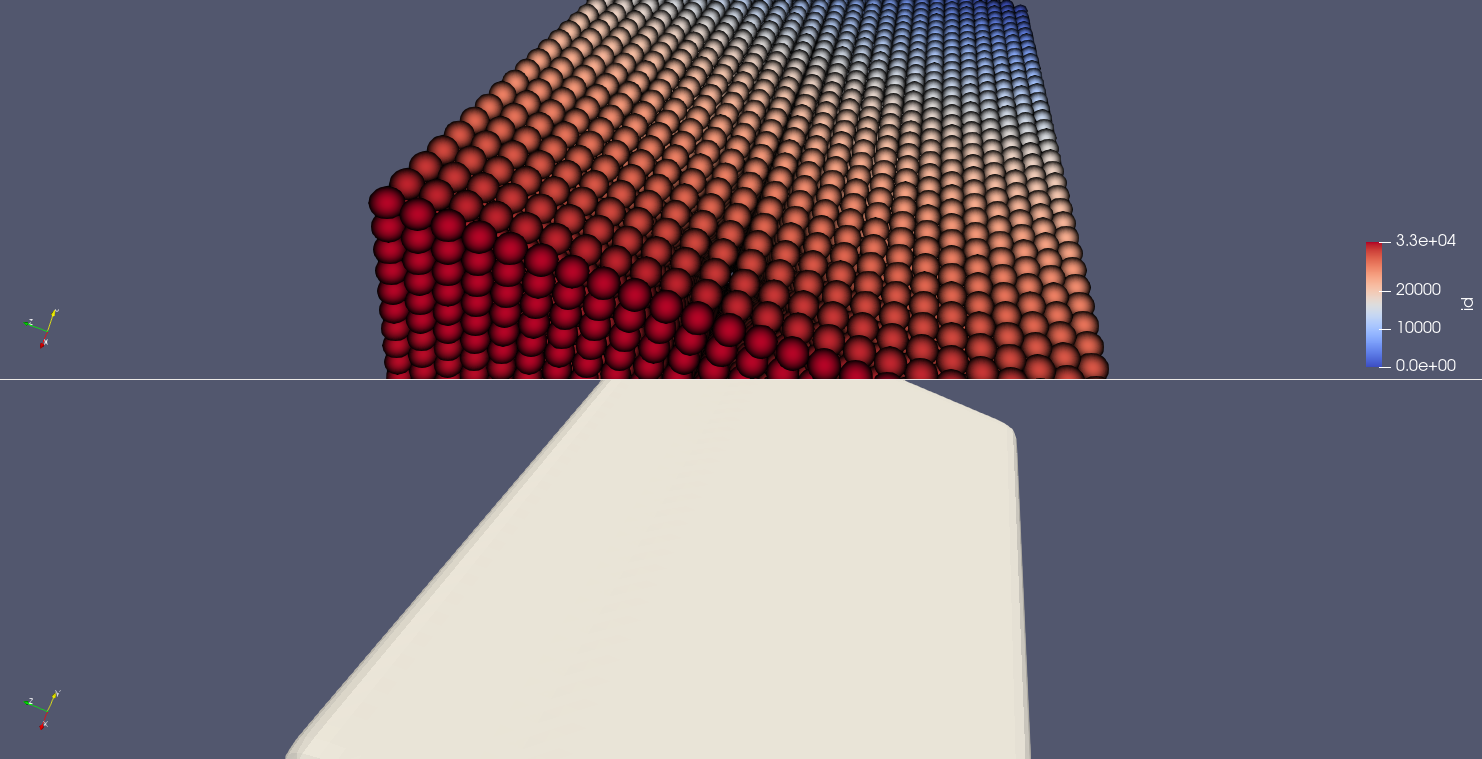
\includegraphics[width=\textwidth]{figures/FlatSurfaceWsParticleDisplacement.png}
			\caption{Regularly displaced particles}
		\end{subfigure}
		\begin{subfigure}[b]{0.6\textwidth}
			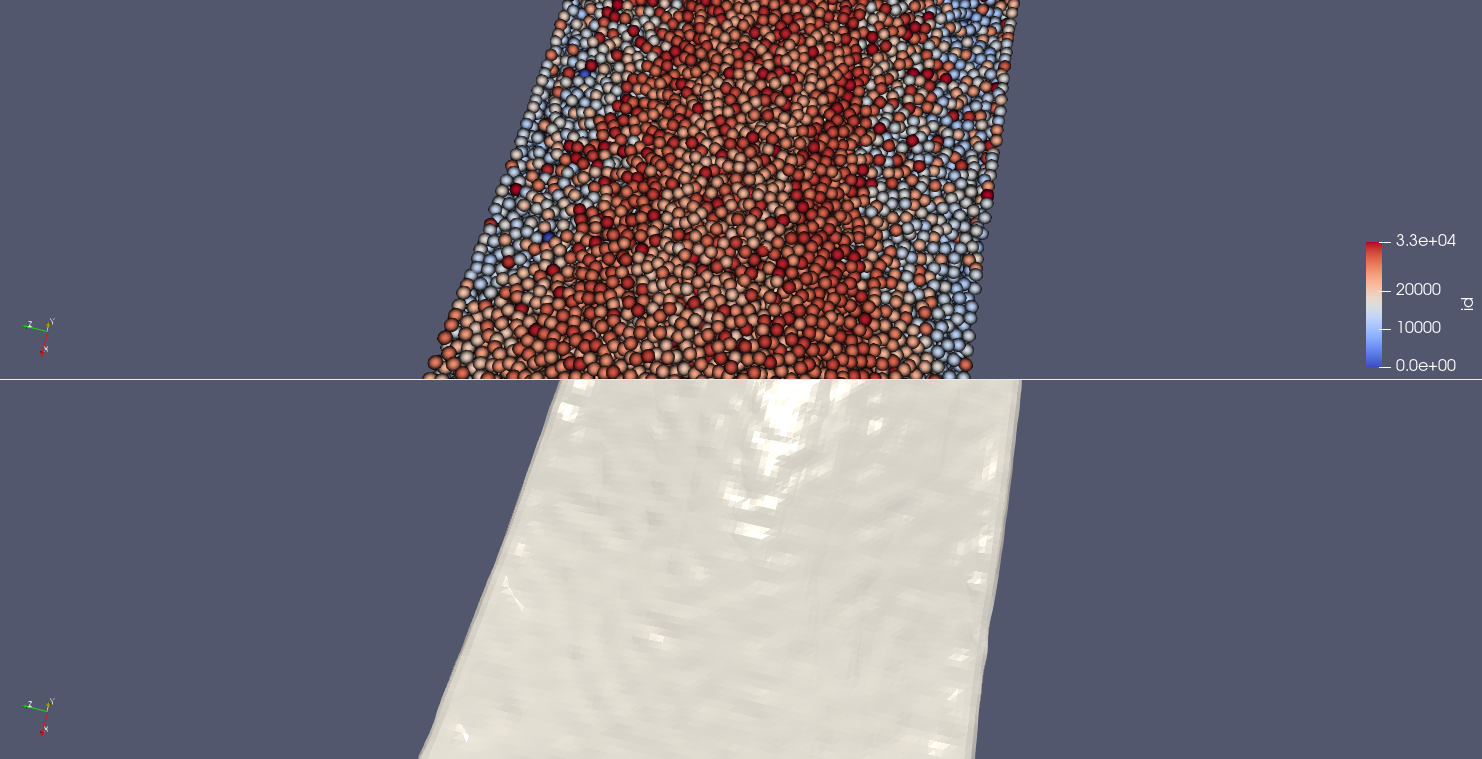
\includegraphics[width=\textwidth]{figures/NonFlatSurfaceWsParticleDisplacement.png}
			\caption{Irregularly displaced particles}
		\end{subfigure}
	\end{center}
	\caption{displacement of particles vs surface quality comparison}
	\label{fig:rec_vs_displacement}
\end{figure}
The main goal of this thesis is to develop a method, which will smooth out a high frequency bumps on flat surface areas, preserving the surface features. The goal of this thesis is also to develop such a method, that will be computationally plausable.\\
The first idea, that was applied to achieve stated requirements is simple blurring technique, which is extensively used in computer graphics, such as Gaussian Blur, Median blur, Bilateral blur or other image filtering techniques. In this chapter Blur-based method will be proposed. 
\section{Algorithm description}
Blur method was incorporated into the research framework according to the class hierarchy in Figure \ref{fig:class-diagam}. According to the class diagram, the method inherits the underlying base method (in our case its Density-Based, Zhu and Bridson, or Solenthaler methods), on top of which the computed level set is blurred.  Algorithm \ref{alg:blur_alg} shows the pseudo-code for \emph{updateLevelSet()}.
\begin{algorithm}[H]
	\scriptsize
	\begin{algorithmic}
		\State $levelSet \gets  BaseClass::initialLevelSet$
		\For{$i \in [0, blurIterations]$}
			\State blurLevelSet(levelSet);
		\EndFor
	\end{algorithmic}
	\caption{$updateLevelSet()$ for level set blurring method}
	\label{alg:blur_alg}
\end{algorithm}
According to Algorithm \ref{alg:blur_alg} blurring of the SDF could be performed arbitrary number of times. The influence of number of iterations will be explained in further section.

The \emph{blurLevelSet()} pseudo-code is explained in Algorithm \ref{alg:blur_level_set}
\begin{algorithm}[H]
	\scriptsize
	\begin{algorithmic}
		\ForAll{$vtx \in MC\_CellDomain$}
			\State $neighbors \gets getNeighbourVertices(vtx);$
			\State $blurredLevelSetValue \gets 0$
			\ForAll{$nbVtx \in neighbors$}
				\State $blurredLevelSetValue\gets blurredLevelSetValue + levelSet[neighborVertex]$
			\EndFor
			\State $blurredLevelSetValue\gets\dfrac{blurredLevelSetValue}{sizeof(neighbors)}$
			\State $sf\gets computeSmoothingFactor()$
			\State $blurredLevelSet[vtx]\gets levecSet[vtx] * (1 - sf) + sf * blurredLevelSetValue;$
		\EndFor
	\end{algorithmic}
	\caption{$updateLevelSet()$ for level set blurring method}
	\label{alg:blur_level_set}
\end{algorithm}
The final blurred level set value in Algorythm \ref{alg:blur_level_set} is a wighted sum between the computed blur level set value and initial level set value.
\subsection{Smoothing factor}
The smoothing factor is a value that determines how much new, blurred SDF value of MC grid vertex will contain its initial SDF value (weighted sum of blurred level set value and initial level set value). As described in \ref{alg:blur_level_set} level set value is updated according to the Equation \ref{eq:level_set_value}.
\begin{equation}
newLS = oldLS \cdot (1 - sf) + blurLS \cdot sf \label{eq:level_set_value}
\end{equation}
In Equation \ref{eq:level_set_value} $sf$ is a smoothing factor or a weight. The smoothing factor itself is calculated according to equation \ref{eq:smooth_factor}.
\begin{equation}
	sf_{vtx} = 1 - (1 - min(1, \dfrac{bsf \cdot fp_{vtx}}{maxFp})^2)^{10} \label{eq:smooth_factor}
\end{equation}
where:
\begin{conditions}
	vtx & vertex for which the smoothing factor is computed\\
	fp_{vtx} & number of neighbor fluid particles within support radius from vtx\\
	maxFp & maximum possible fluid particles that can be in the neighborhood of the vertex \\
	bsf & base support factor (use defined)
\end{conditions}
The smoothing factor formula was designed such that it should be maximal for MC grid vertices that contains full fluid particles set and minimum where number of fluid particles limits to zero (see Figure \ref{fig:sf_function_graph}).
\begin{figure}[H]
	\begin{center}
			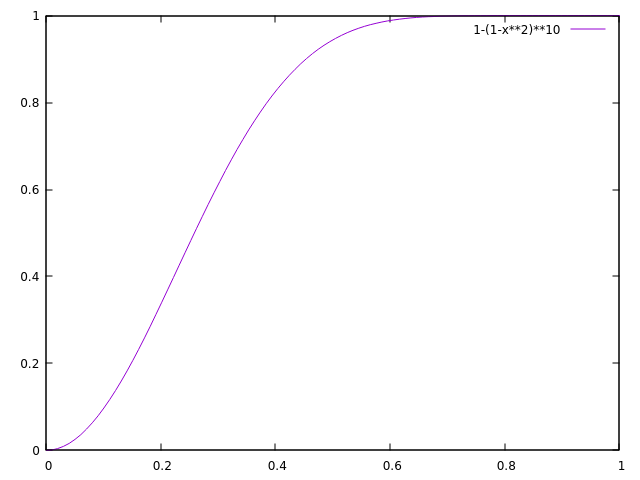
\includegraphics[width=0.5\textwidth]{figures/sf_function_graph.png}		
	\end{center}
	\caption{Graphic of function, representing equation \ref{eq:smooth_factor}. Taking into account that $min(1, \dfrac{bsf \cdot fp_{vtx}}{maxFp}) \in [0,1]$ the function converges from 0 to 1 in the interval $x \in [0, 0.5]$ and limits to 1 for the area $x\in [0.5, 1]$}
	\label{fig:sf_function_graph}
\end{figure}

The motivation to apply such a smoothing factor comes from the problem of the blurring algorithm. If we apply the blur algorithm uniformly into all MC domain, the blur will smooth out the features in thin areas and the areas with a small set of particles (droplets or splashes). Figure \ref{fig:smoothing_factor_influence} shows the problem of application of the blur algorithm w.o. application of smoothing factor.

\begin{figure}[H]
	\begin{center}
			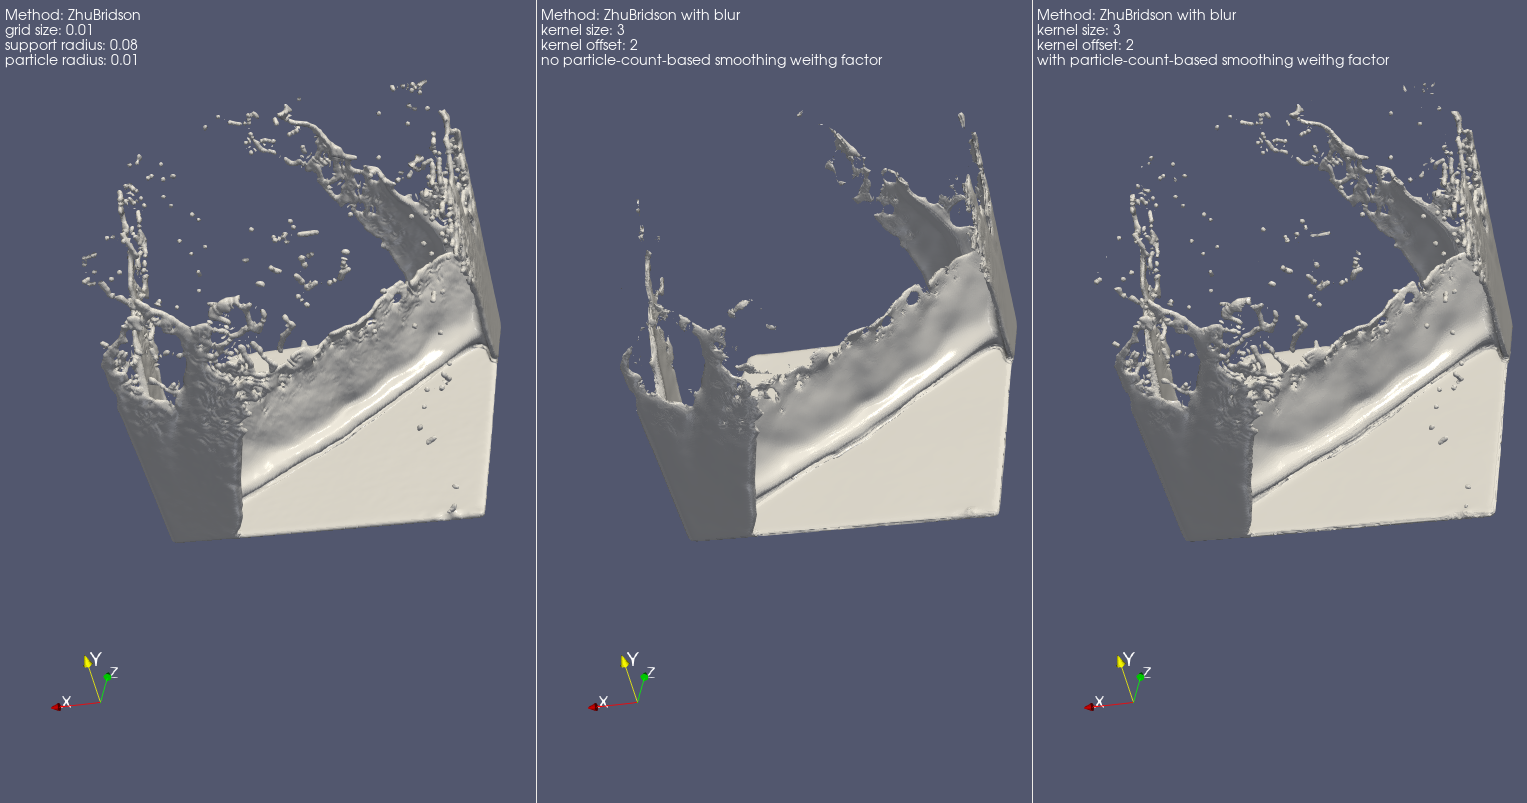
\includegraphics[width=\textwidth]{figures/View2.png}		
	\end{center}
	\caption{Leftmost is initial Zhu and Bridson reconstruction, middle - blur reconstruction w.o. smoothing factor application, rightmost - blur reconstruction with usage of smoothing factor}
	\label{fig:smoothing_factor_influence}
\end{figure}


The idea of blurring using a smoothing factor is to blur the level set as much as possible in the areas where the surface of the fluid is flat and to apply less blur in areas, where a set of MC cells lacks fluid particles. Suppose the general case in Figure \ref{fig:sf_example}. In the figure red, yellow and orange grid vertices contain a full, half and quarter set of particles respectively. Level set values of the grid points are supposed to be blurred as much as possible near the flat fluid surface areas, but left unchanged in areas with small set of particles.
\begin{figure}[H]
	\begin{center}
		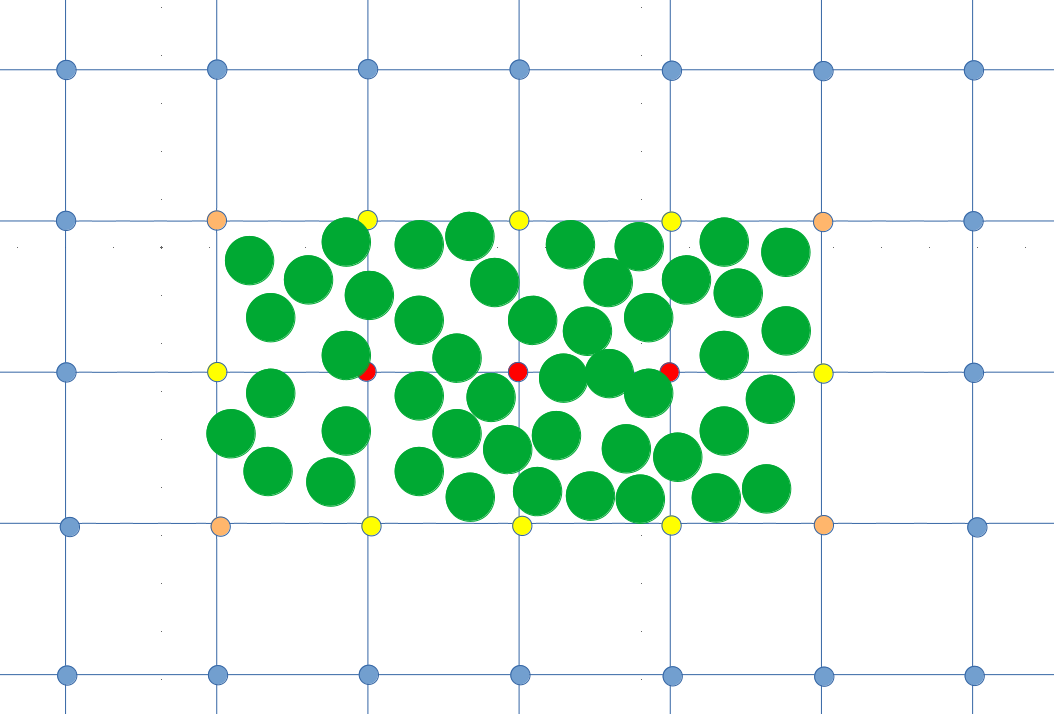
\includegraphics[width=0.5\textwidth]{figures/SmoothingFactorPictureExplenation.png}		
		\caption{Green circles are fluid particles, red - MC cells with full set of fluid particles in the neighborhood, yellow -  MC cells with half set of fluid particles in the neighborhood, orange - MC cells with quarter set of fluid particles in the neighborhood, blue - MC cells with no fluid particles in the neighborhood}
		\label{fig:sf_example}
	\end{center}
\end{figure}
Applying blur to the level set vertices that are inside the fluid (and all its neighbor cells are also inside the fluid) will not change the level set value too much as soon all vertices that has full set of fluid particles in the neighborhood will have similar level set values.\\
For the MC vertices that are near the corners the 75\% of the neighbor vertices are outside the fluid. In this case blur iteration will bias the vertex outside the fluid, thus the fluid will shrink. This is also relevant for the thin areas and splashes.\\
At the figure \ref{fig:blur_w_o_sf} the effect of surface shrinkage of applying blur in the thin area and in the corners w.r.t. the initial reconstruction method can be observed. The flat surface is smoothed out, but at the same time surface sharpness at the thin and splash areas is degraded, some small features/droplets are lost.
\begin{figure}[H]
	\begin{center}
		\begin{subfigure}[b]{\textwidth}
			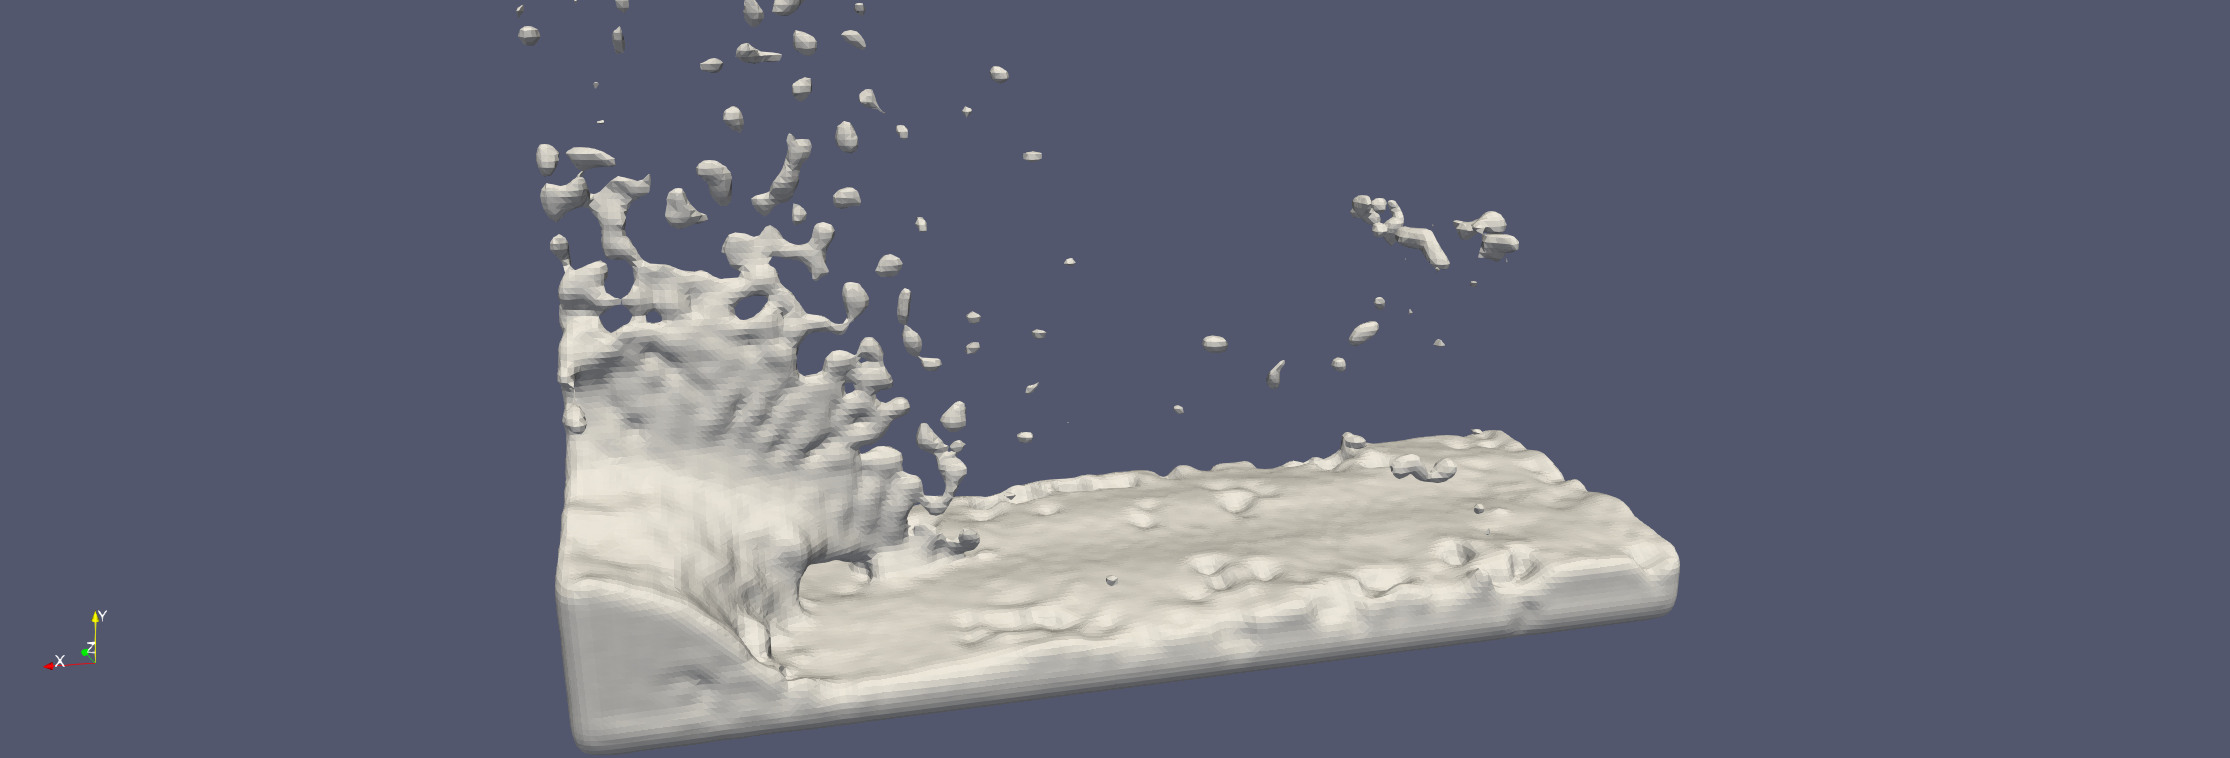
\includegraphics[width=\textwidth]{figures/DenvityBlurredSplashArea.png}
			\caption{Density based surface reconstruction}
			\label{fig:denc_rec}
		\end{subfigure}
		\begin{subfigure}[b]{\textwidth}
			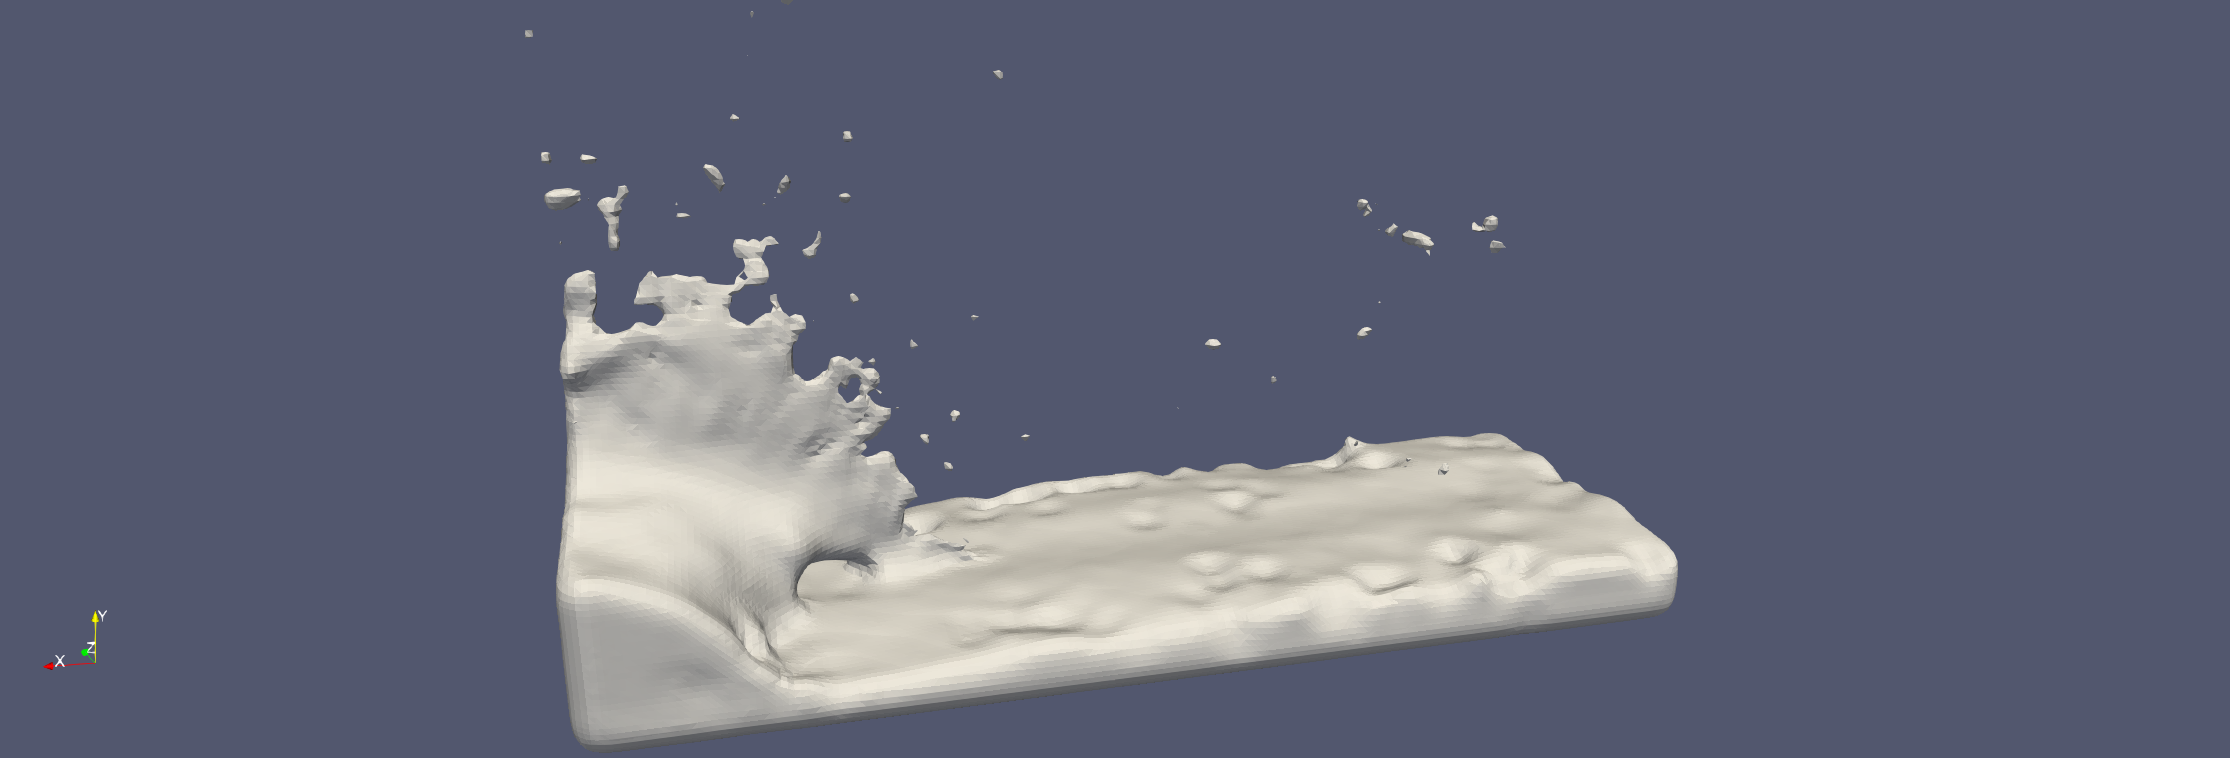
\includegraphics[width=\textwidth]{figures/DenvityBasedSplashArea.png}
			\caption{Density based surface reconstruction with blur (smoothing factor is not applied)}
			\label{fig:blur_w_o_sf}
		\end{subfigure}
	\end{center}
	\caption{Comparison of original reconstruction method and blurred reconstruction without application of smoothing factor}
	\label{fig:blur_thin_area}
\end{figure}
In the other hand applying blur on level set with smoothing factor smooths out the flat surface areas bumps, but preserves small feature areas (see Figure \ref{fig:blur_thin_area_with_sf}).
\begin{figure}[H]
        \begin{subfigure}[b]{0.5\textwidth}
               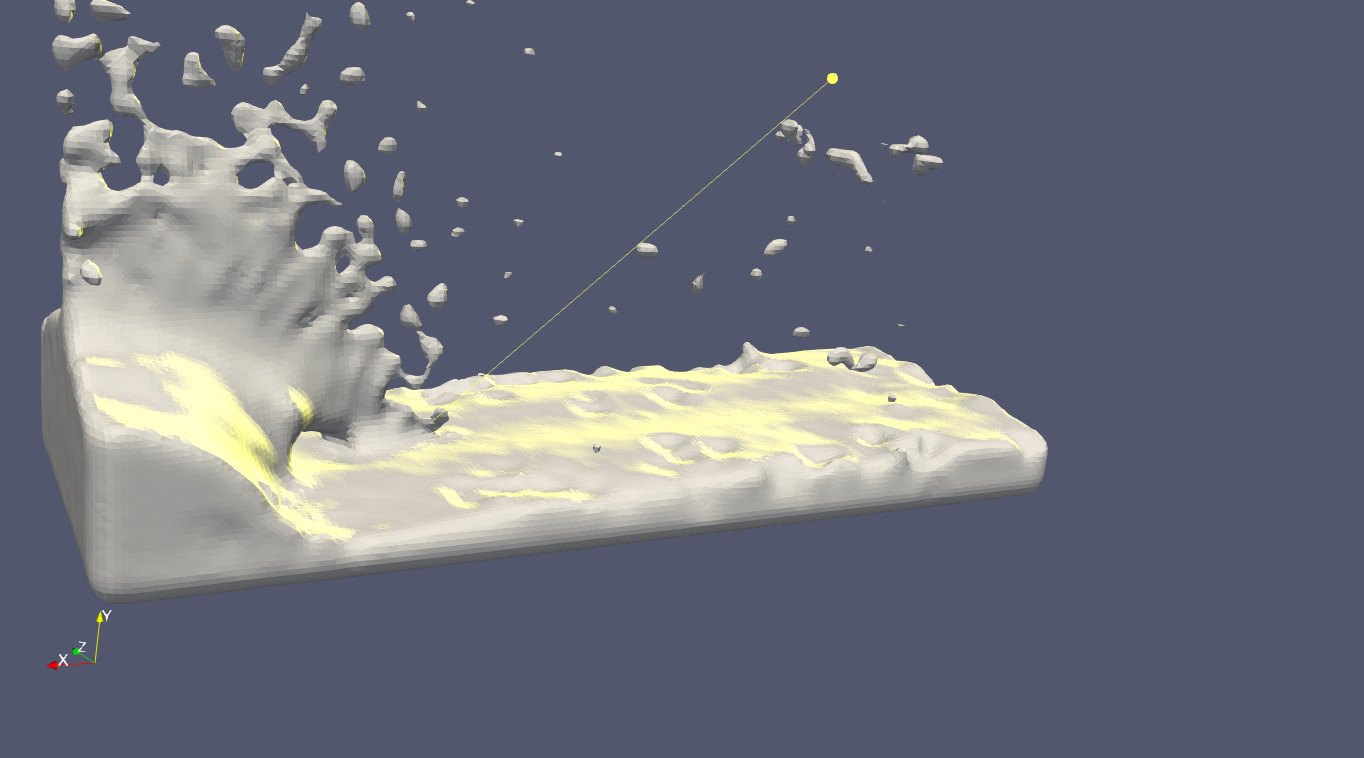
\includegraphics[width=\textwidth]{figures/DenvityBasedSplashArea2.png}
               \caption{Density based surface}
               \label{fig:db_rec}
        \end{subfigure}
        \begin{subfigure}[b]{0.5\textwidth}
               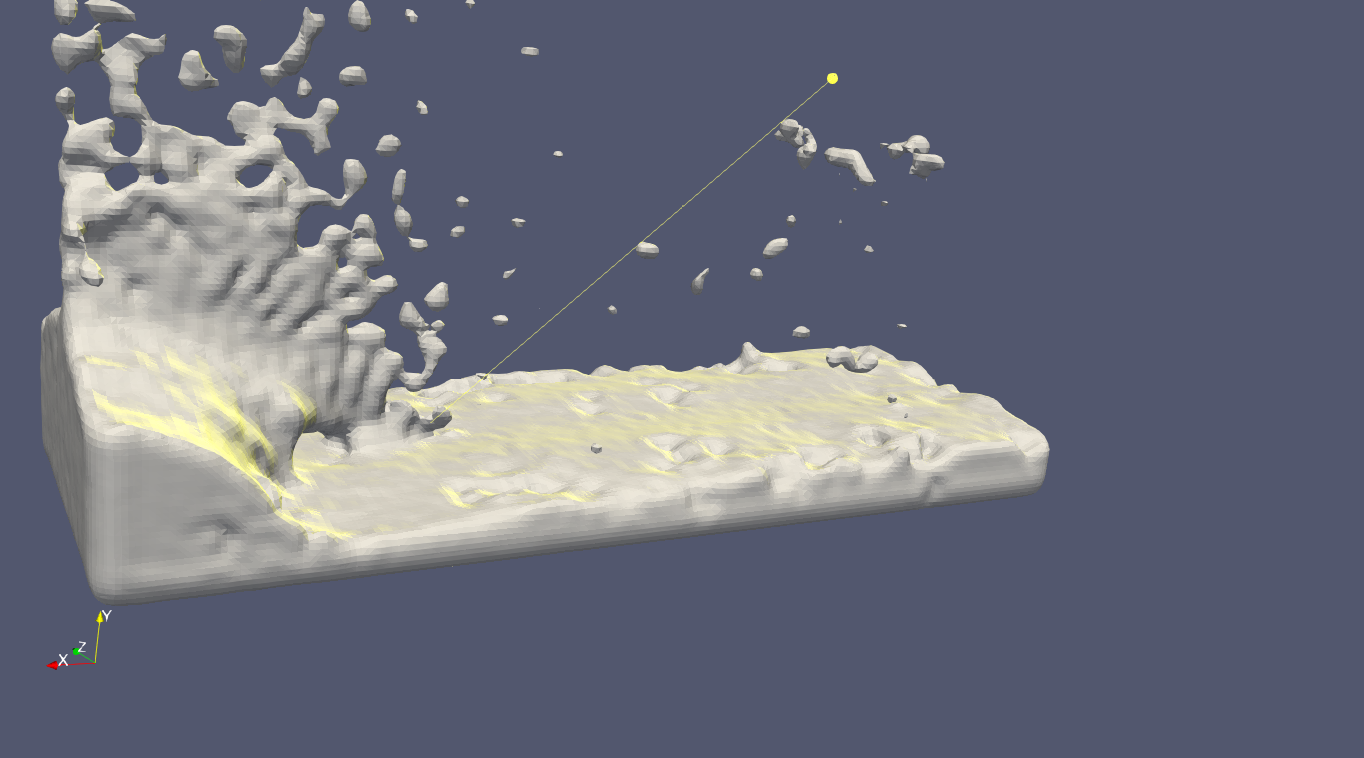
\includegraphics[width=\textwidth]{figures/DenvityBlurredSplashArea2.png}
               \caption{Applying smoothing factor to level set blur}
				\label{fig:blur_with_sf}
        \end{subfigure}
       \caption{Comparison of original reconstruction method and blurred reconstruction with application of smoothing factor}
       \label{fig:blur_thin_area_with_sf}
 \end{figure}
 \subsection{Neighbors detection algorithm}
In the Algorithm \ref{alg:blur_level_set} MC neighbor vertices are computed in function $getNeighbourVertices(vtx)$. The Algorithm \ref{alg:blur_nbs_search} describes the procedure of neighbors detection procedure.
\begin{algorithm}[H]
	\scriptsize
	\begin{algorithmic}
		\State $neighbors \gets \{vtx\}$
		\State $sdfGradient \gets \nabla_x sdf(vtx)$
		\If{$sdfGradient \cdot sdfGradient < 1e-6$}
			\State $return\ neighbors$
		\EndIf
		\State $Normalize sdfGradient$
		
		\For{$i \in [-kernelSize \cdot kernelOffset, kernelSize \cdot kernelOffset]$, $stepsize = kernelOffset$}
			\For{$j \in [-kernelSize \cdot kernelOffset, kernelSize \cdot kernelOffset]$, $stepsize = kernelOffset$}
				\For{$k \in [-kernelSize \cdot kernelOffset, kernelSize \cdot kernelOffset]$, $stepsize = kernelOffset$}
					\If{$i = 0 \land j = 0 \land k = 0$}
						\State $neighbors \gets neighbors \cup vtx$
						\State $continue$
					\EndIf
					
					\State $offsetVector \gets [i \cdot GridResolution, j \cdot GridResolution, k \cdot GridResolution]$;
					\If{$offsetVector \cdot sdfGradient \geq kernelDepth \cdot kernelSize \cdot GridResolution$}
						\State $continue$
					\EndIf
					
					\State $neighbors \gets neighbors \cup (vtx + offsetVector)$
				\EndFor
			\EndFor
		\EndFor
		\State $return\ neighbors$
	\end{algorithmic}
	\caption{neighborhood search for level set blur algorithm}
	\label{alg:blur_nbs_search}
\end{algorithm}
\textcolor{red}{TODO: add more explanations}
The algorithm traverses along all neighbor MC grid vertices within kernel size and kernel offset. It filters out a mesh vertices that are too fare from the reference vertex in a normal direction within a kernel depth. The normal is computed using a gradient of SDF in reference point. Well known forward differences are used to compute a gradient for the base vertex.
\begin{equation}
	\dfrac{\partial \phi}{\partial x} = \dfrac{\phi_{i+1} - \phi_i}{x_{i+1} - x_i}
\end{equation}
After computation of the gradient it is normalized, while only the unit normal is required. There is a degenerate case, when computed gradient vanishes. To handle this case computation of neighbors is imply skipped, and original SDF value is applied. After all, the probability of occurrence of such an event is too small. Figure \ref{fig:nghbrs_computation} shows the example of neighbors displacement with kernel size 3 and kernel depth 0.5.
\begin{figure}[H]
    \begin{subfigure}[b]{0.5\textwidth}
           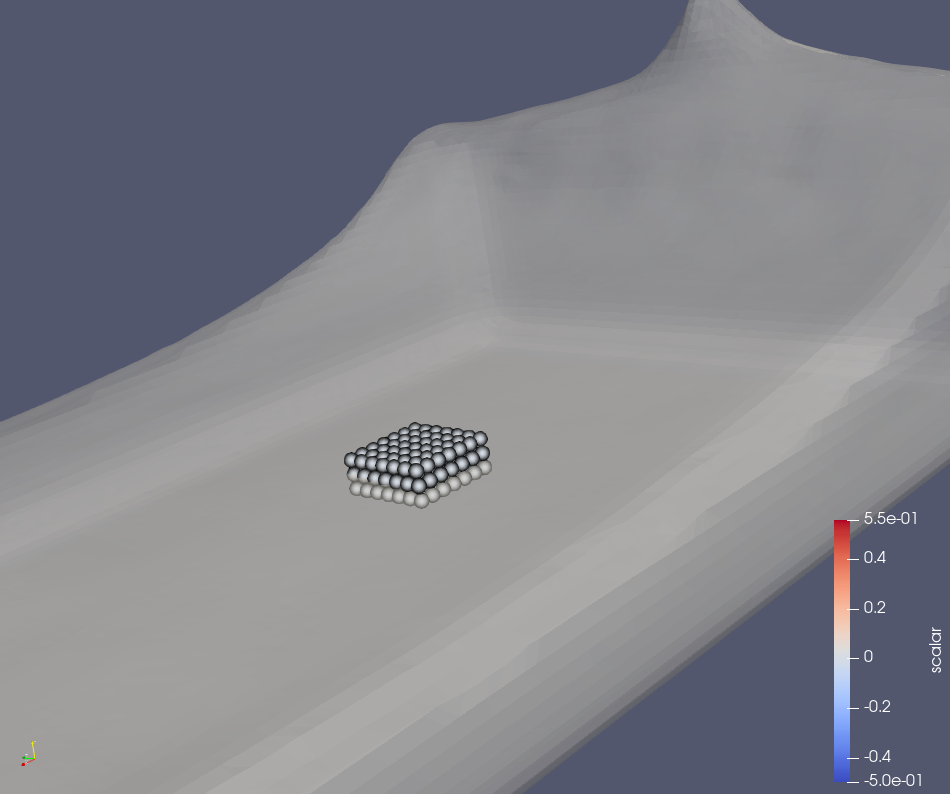
\includegraphics[width=\textwidth]{figures/NeighborsComputation.png}
    \end{subfigure}
    \begin{subfigure}[b]{0.5\textwidth}
           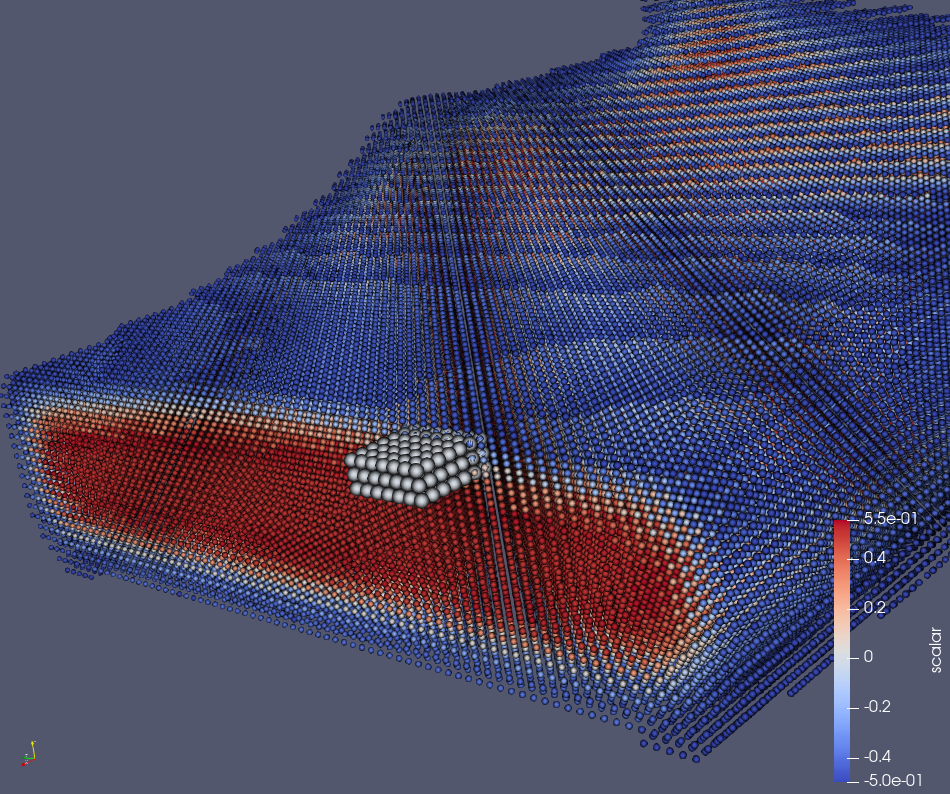
\includegraphics[width=\textwidth]{figures/NeighborsComputation2.png}
    \end{subfigure}

    \caption{resulting neighbors computed for one of the MC grid vertices (white points are computed neighbors)}
    \label{fig:nghbrs_computation}
\end{figure}
\subsection{Blur kernel size and offset}
The kernel size and kernel offset concept is widely used in a computer graphics blur algorithms. It is a widely used effect in graphics software, typically to reduce image noise and reduce detail. The visual effect of this blurring technique is a smooth blur resembling that of viewing the image through a translucent screen.\\
The most popular blur technique applied in computer graphics is a Gaussian blur. Mathematically, applying a Gaussian blur to an image is the same as convolving the image with a Gaussian function. This is also known as a two-dimensional Weierstrass transform.\\
Each pixel in the image gets multiplied by the Gaussian kernel. This is done by placing the center pixel of the kernel on the image pixel and multiplying the values in the original image with the pixels in the kernel that overlap. The values resulting from these multiplications are added up and that result is used for the value at the destination pixel.\\
The kernel could be of an arbitrary size, e.g. uniform box kernel with kernel size 1: 
$\begin{pmatrix}
1 & 1 & 1\\
1 & 1 & 1\\
1 & 1 & 1
\end{pmatrix}$, kernel size 2: 
$\begin{pmatrix}
1 & 1 & 1 & 1 & 1\\
1 & 1 & 1 & 1 & 1\\
1 & 1 & 1 & 1 & 1\\
1 & 1 & 1 & 1 & 1\\
1 & 1 & 1 & 1 & 1
\end{pmatrix}$. This could be easely extended to a 3D case, which is useful in this work.\\
The kernel offset, can be expressed as a smallest amount of steps over the neighborhood that should be performed to reach next sample, which will be used in blurring procedure. E.g. next matrix describes a kernel with kernel size 1 and kernel offset 2 : $
\begin{pmatrix}
	1 & 0 & 1 & 0 & 1\\
	0 & 0 & 0 & 0 & 0\\
	1 & 0 & 1 & 0 & 1\\
	0 & 0 & 0 & 0 & 0\\
	1 & 0 & 1 & 0 & 1
\end{pmatrix}
$.\\
Both parameter influences a quality of a surface reconstruction. However kernel size also defines the runtime quality of the algorythm, as soon as kernel performance of the blur stageover the SDF depends cubically on the kernel size the total complexity of the blur stage can be expressed as $O(n\cdot k^3)$, where n is a number of MC grid vertices $k$ is a kernel size. In the other hand kernel offset doesn't influences the performance of the SDF blurring stage, as soon as according to the Algorithm \ref{alg:blur_nbs_search} it doesn't influences on the number of samples that will be picked for blurring.\\
However expansion of the kernel size/offset has its limitation on the surface quality from smoothing out a sharp features up to bringing artifacts to the reconstructed surface. Figure \ref{fig:ksko} shows reconstructed surface with different evaluation of a kernel size and kernel offset.\\
\begin{figure}[H]
        \begin{subfigure}[b]{0.5\textwidth}
               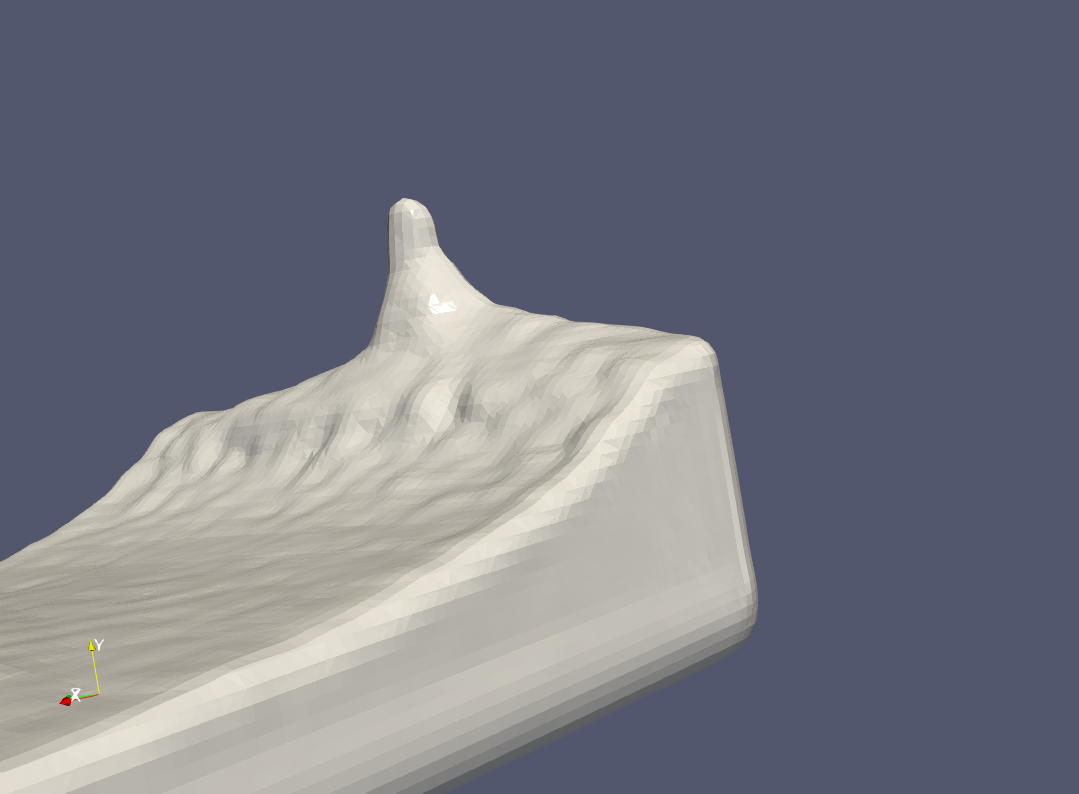
\includegraphics[width=\textwidth]{figures/DBBlur_ks-0_ko-0.png}
               \caption{Original reconstruction}
               \label{fig:kskdOrig}
        \end{subfigure}
        \begin{subfigure}[b]{0.5\textwidth}
               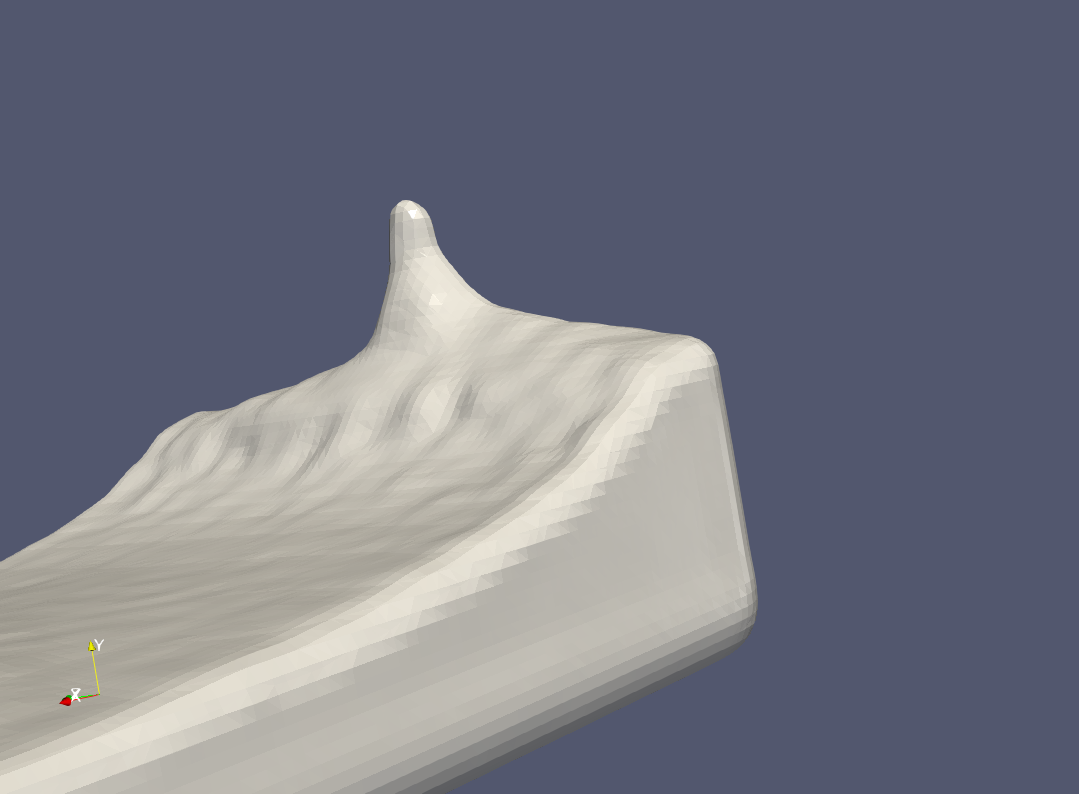
\includegraphics[width=\textwidth]{figures/DBBlur_ks-1_ko-1.png}
               \caption{kernel size 1, kernel offset 1}
               \label{fig:ks1ko1}
        \end{subfigure}
        \begin{subfigure}[b]{0.5\textwidth}
               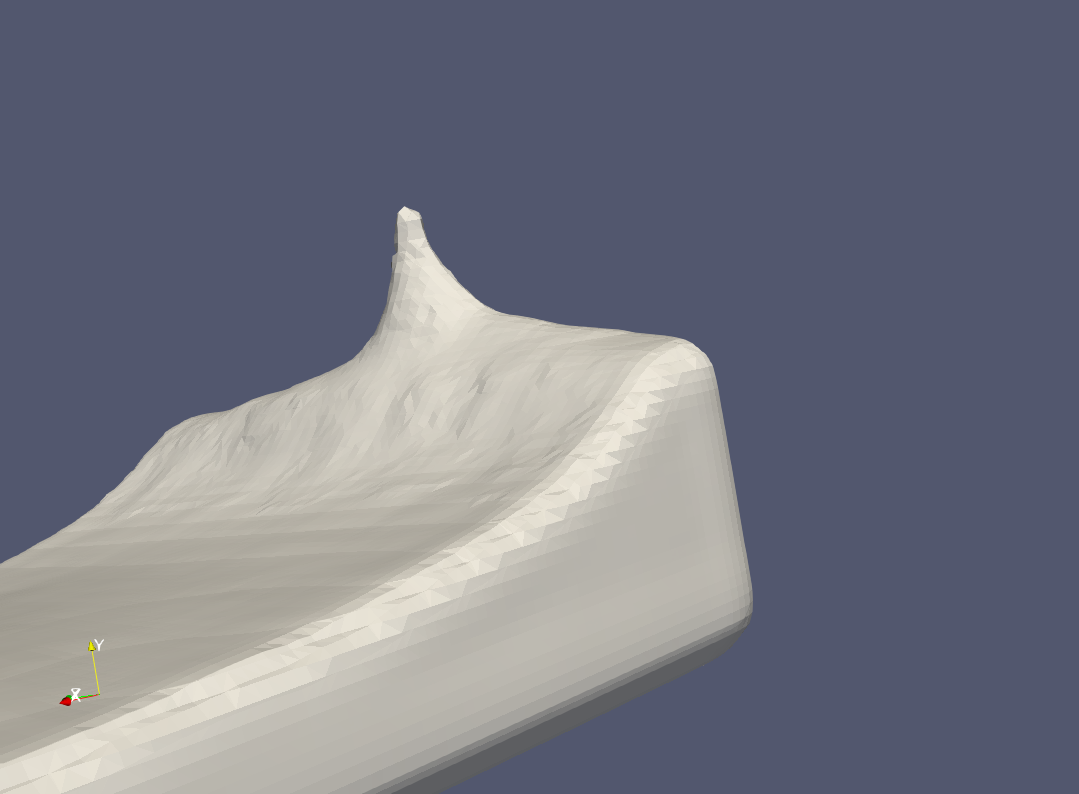
\includegraphics[width=\textwidth]{figures/DBBlur_ks-1_ko-2.png}
               \caption{kernel size 1, kernel offset 2}
               \label{fig:ks1ko2}
        \end{subfigure}
        \begin{subfigure}[b]{0.5\textwidth}
               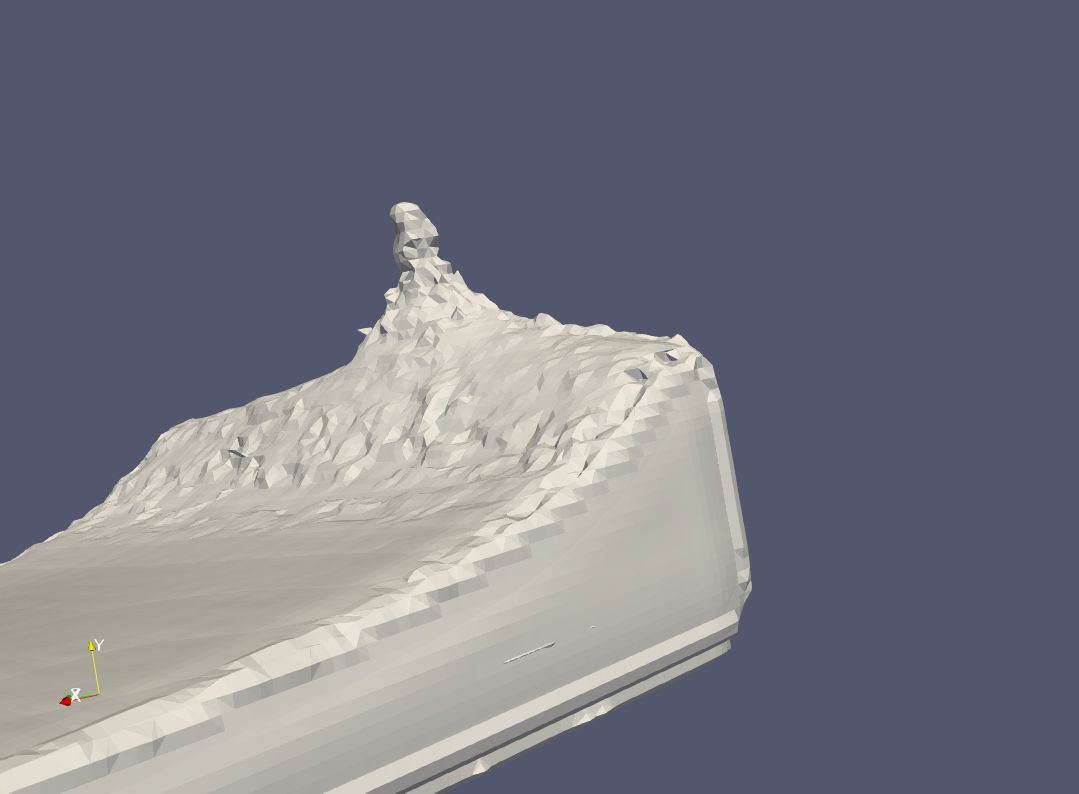
\includegraphics[width=\textwidth]{figures/DBBlur_ks-1_ko-4.png}
               \caption{kernel size 1, kernel offset 4}
               \label{fig:ks1ko4}
        \end{subfigure}
        \begin{subfigure}[b]{0.5\textwidth}
               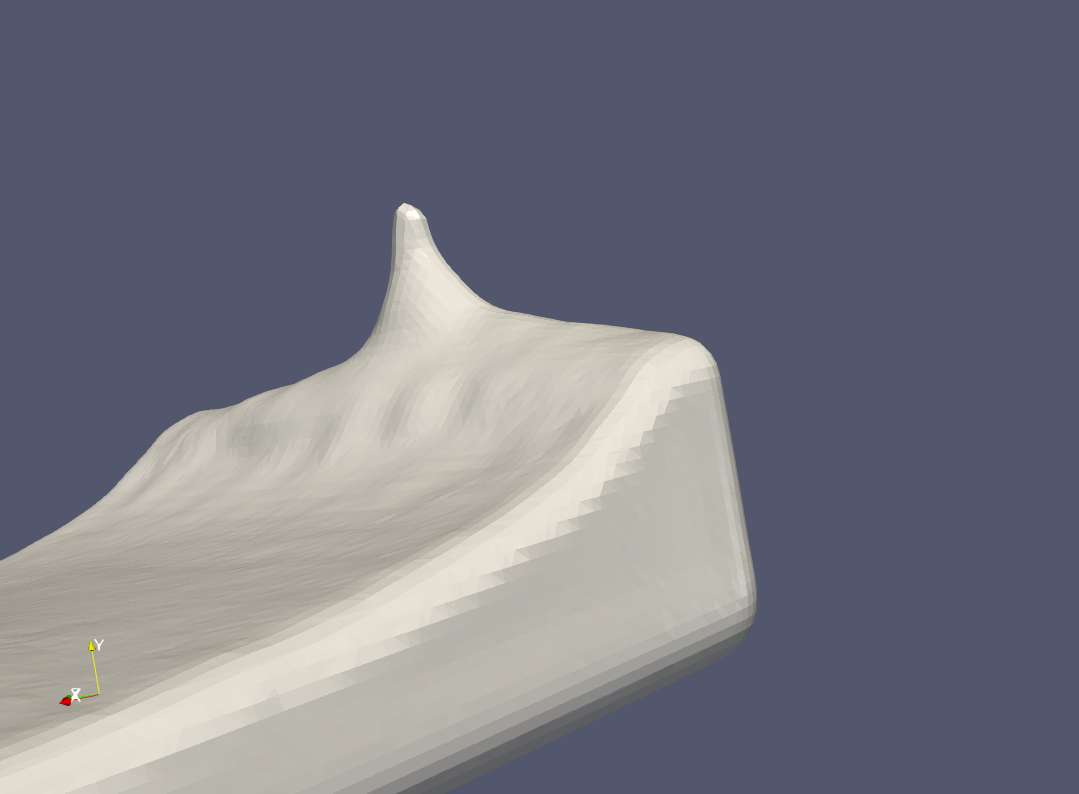
\includegraphics[width=\textwidth]{figures/DBBlur_ks-2_ko-1.png}
               \caption{kernel size 2, kernel offset 1}
               \label{fig:ks2ko1}
        \end{subfigure}        
        \begin{subfigure}[b]{0.5\textwidth}
               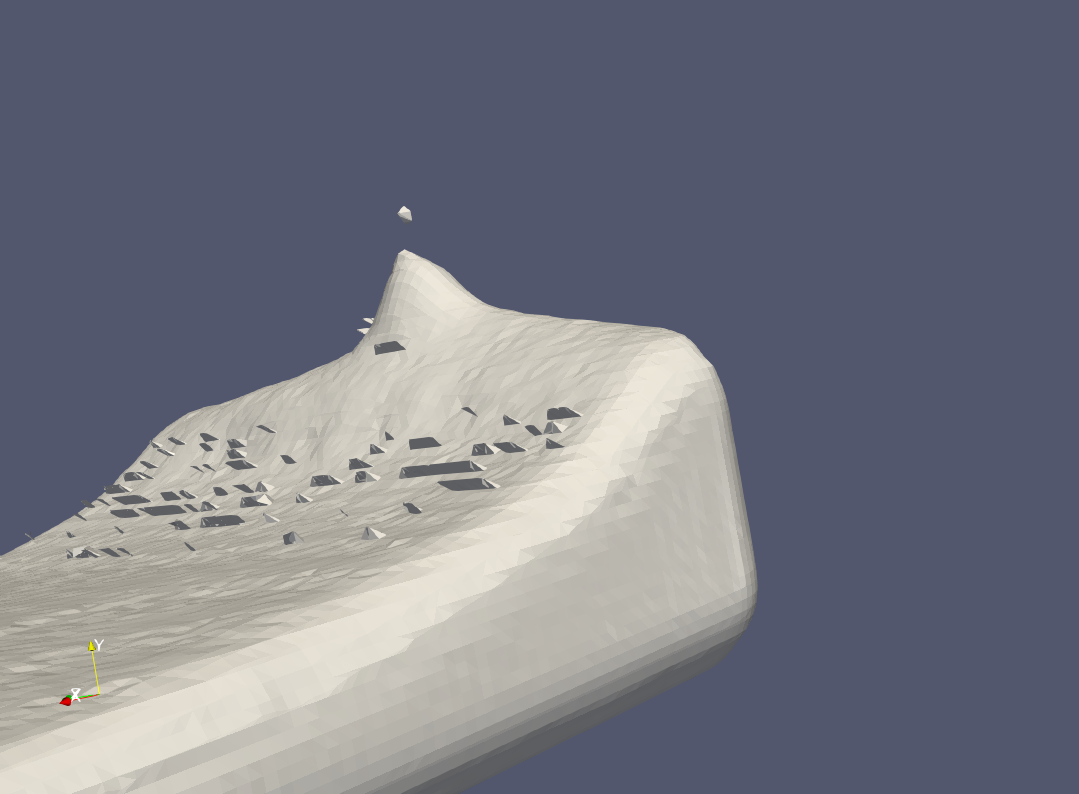
\includegraphics[width=\textwidth]{figures/DBBlur_ks-4_ko-1.png}
               \caption{kernel size 4, kernel offset 1}
               \label{fig:ks4ko1}
        \end{subfigure}
        \caption{Kernel size and kernel offset reconstruction comparison}
        \label{fig:ksko}
\end{figure}
If the kernel size or a kernel offset i taken too large, so that the MC grid is out of bounds of the simulation, then SDF values of MC vertices near to the bounds of the grid will be biased too much to the fluid forming holes or parasite surfaces as in Figures \ref{fig:ks4ko1} and \ref{fig:ks1ko4}.
\subsection{Kernel depth}
The advantage of the static MC grid is that it has a static displacement of all grid vertices, thus the neighborhood can be efficiently computed. However, using the full neighborhood within the $kernelSize$ and $kernelOffset$ is not sufficient for level set blurring. As soon as the smoothing aims to remove bumps in the flat surface areas it is more practical to take into account level set vertices, that are in the neighborhood of the fluid surface. Thus, for each vertex of the level set gradient of the level set can be computed.
The gradient of the implicit function for the SDF is defined as
\begin{equation}
	\nabla\phi = \left( \dfrac{\partial\phi}{\partial x}, \dfrac{\partial\phi}{\partial y}, \dfrac{\partial\phi}{\partial z}\right)
\end{equation}
The gradient $\nabla\phi$ is perpendicular to the isocontours of $\phi$ and points in the
direction of increasing $\phi$. Therefore, if $x_0$ is a point on the zero isocontour
of $\phi$, i.e., a point on the fluid surface, then $\nabla\phi$ evaluated at $x_0$ is a vector that points in the same direction as the local unit (outward) normal N to the interface. Thus, the unit (outward) normal for points on the interface is \cite{LevelSetMethods}
\begin{equation}
	N = \dfrac{\nabla\phi}{|\nabla \phi|}
\end{equation}

For flat surface areas it is convenient to blur SDF vertex values w.r.t. vertices, which resides in a tangential direction to the surface normal.

\begin{figure}[H]
        \begin{subfigure}[b]{0.5\textwidth}
               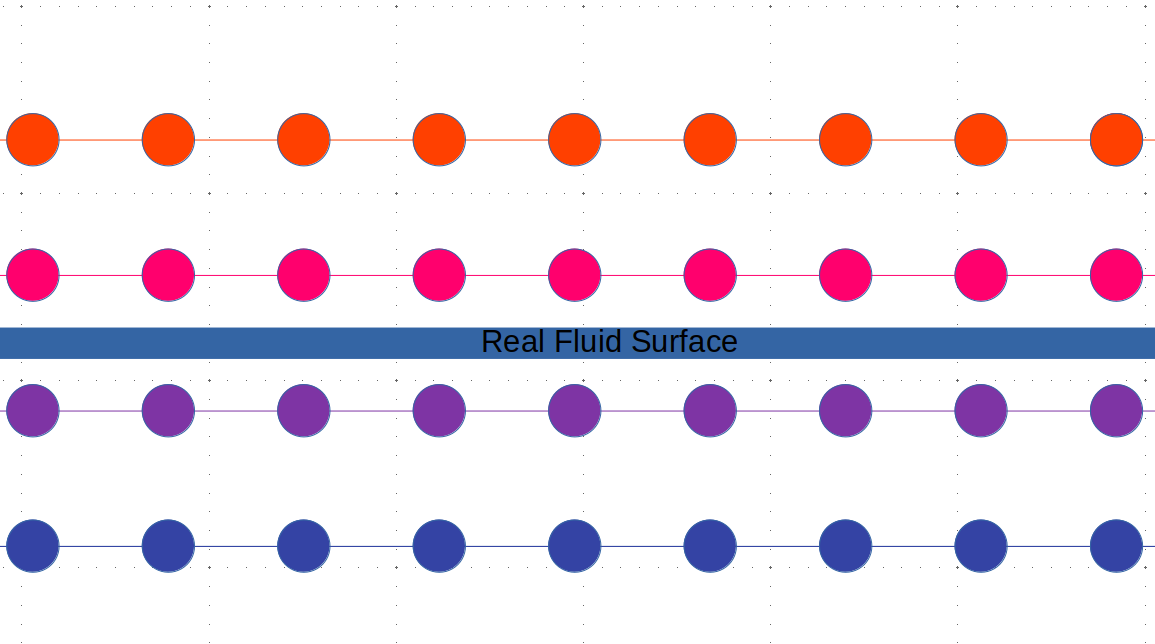
\includegraphics[width=\textwidth]{figures/RealFluidSurfaceLevelSet.png}
               \caption{Expected reconstruction of flat surface}
               \label{fig:expected_fs}
        \end{subfigure}
        \begin{subfigure}[b]{0.5\textwidth}
               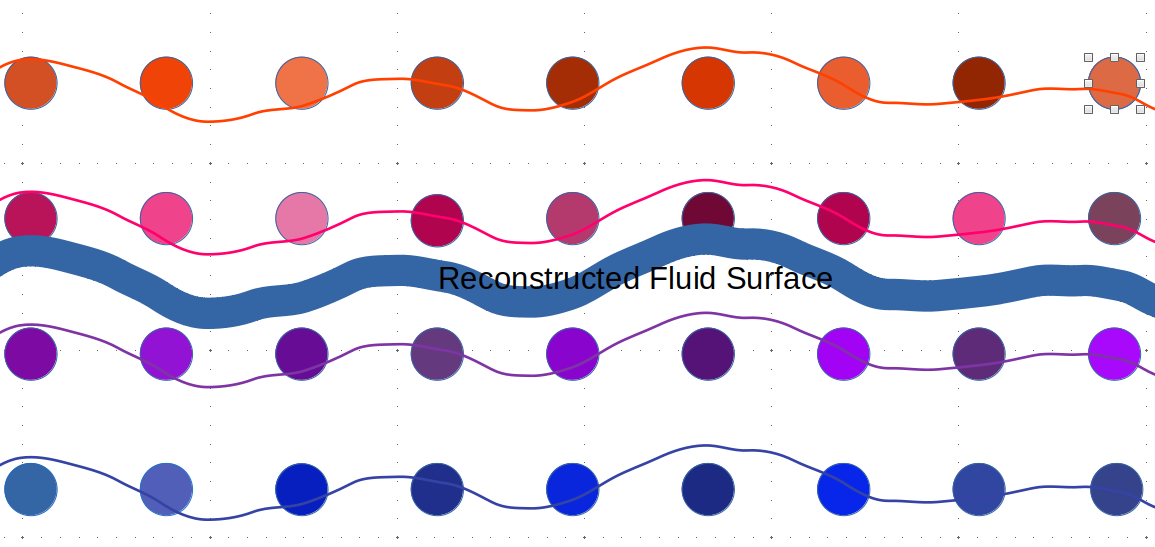
\includegraphics[width=\textwidth]{figures/ReconstructedFluidSurface.png}
               \caption{Bumpy reconstruction of flat surface}
				\label{fig:recon_fs}
        \end{subfigure}
        \begin{subfigure}[b]{0.5\textwidth}
               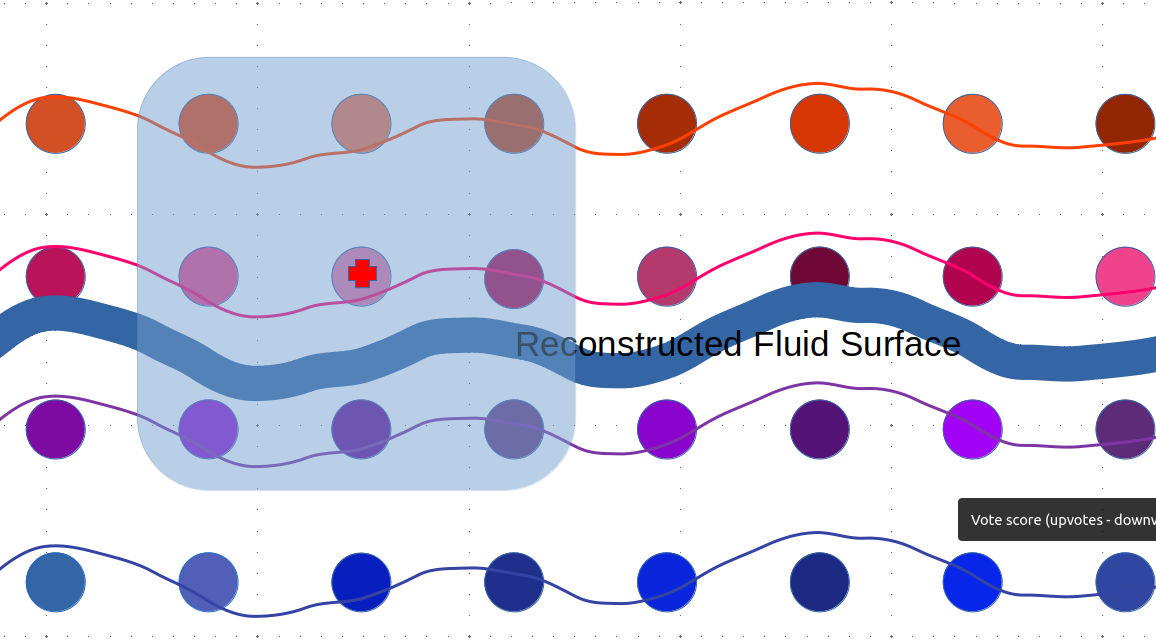
\includegraphics[width=\textwidth]{figures/LevelSetBlurFullKernel.png}
               \caption{Application of full kernel size}
               \label{fig:full_ks}
        \end{subfigure}
        \begin{subfigure}[b]{0.5\textwidth}
               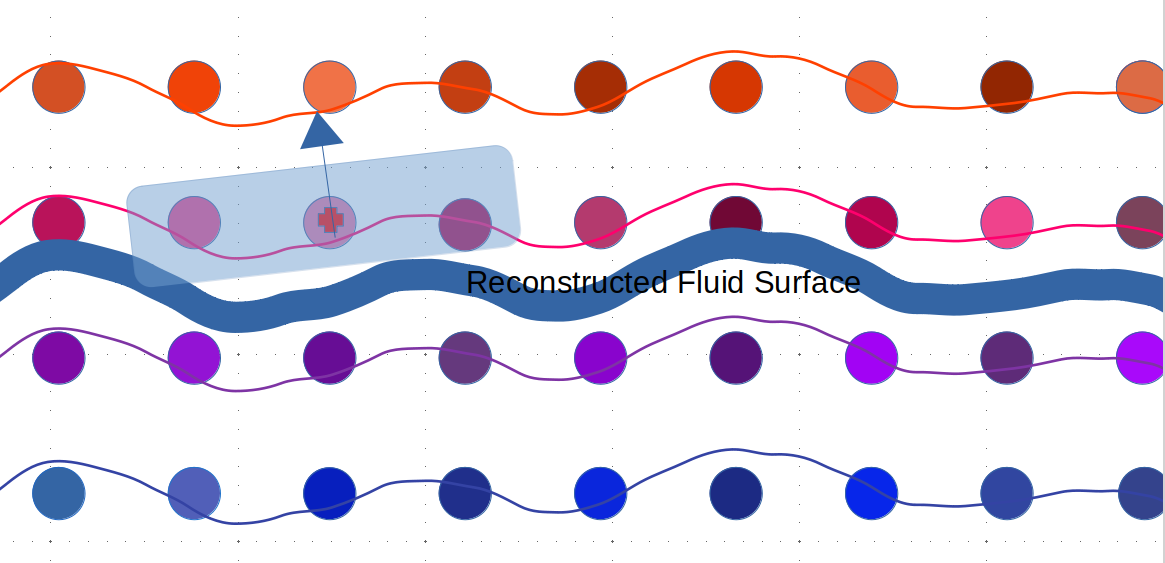
\includegraphics[width=\textwidth]{figures/LevelSetBlurKernelPart.png}
               \caption{Adjustment kernel in normal direction to iso-surface}
				\label{fig:partial_ks}
        \end{subfigure}

       \caption{Colored lines are iso-surface levels. Dots are MC grid vertices with their respective level set values}
       \label{fig:kd_surface_explenation}
 \end{figure}
At the Figure \ref{fig:expected_fs} expected iso-surface in flat fluid area is displayed. Dots of different colors are the MC grid vertices. Colors represent the level set value. In the perfect case level set ISO-lines (in the 2D example) forms straight lines, thus MC grid vertices along the iso-line will receive similar SDF evaluations. However, due to the irregular displacement of fluid particles surface is usually reconstructed as shown in Figure \ref{fig:recon_fs}. In case if we apply full kernel size (see Figure \ref{fig:full_ks}) we will pick level set values from different iso-surface levels, which will change level set values unpredictably.\\
The better approach is to pick a kernel frame so that only level set values of near-surface MC vertices will be used for blur operation (Figure \ref{fig:partial_ks}). This way blur operation will smooth out grid vertices along the iso lines. Especially the influence of the kernel depth can be seen in thin areas, where kernel frame is larger than a thickness of a fluid surface (see Figure \ref{fig:kd_influence example}).
\begin{figure}[H]
        \begin{subfigure}[b]{1\textwidth}
               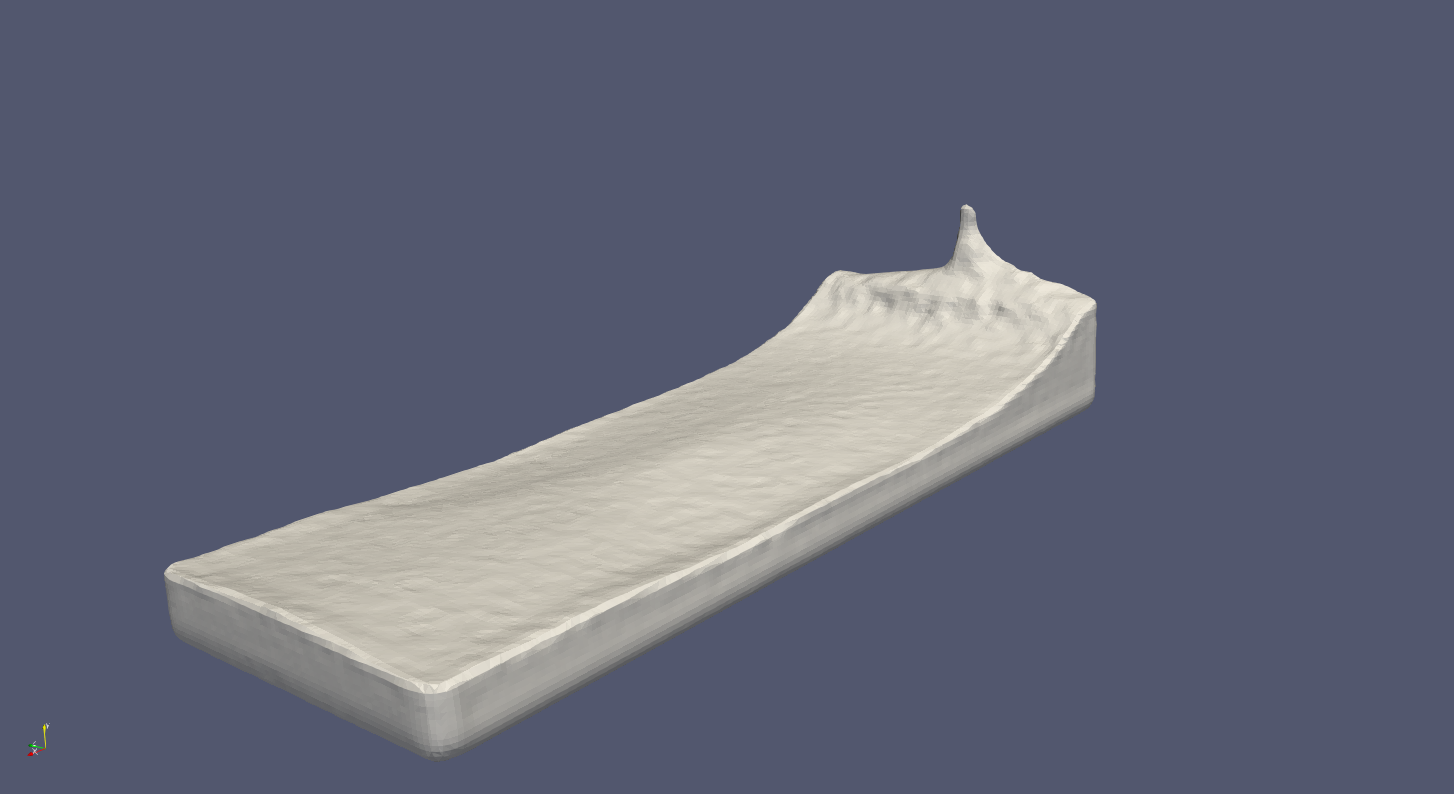
\includegraphics[width=\textwidth]{figures/KernelDepthOriginalReconstruction.png}
               \caption{Original ZhuBridson reconstruction}
               \label{fig:kd_original}
        \end{subfigure}
        \begin{subfigure}[b]{0.5\textwidth}
               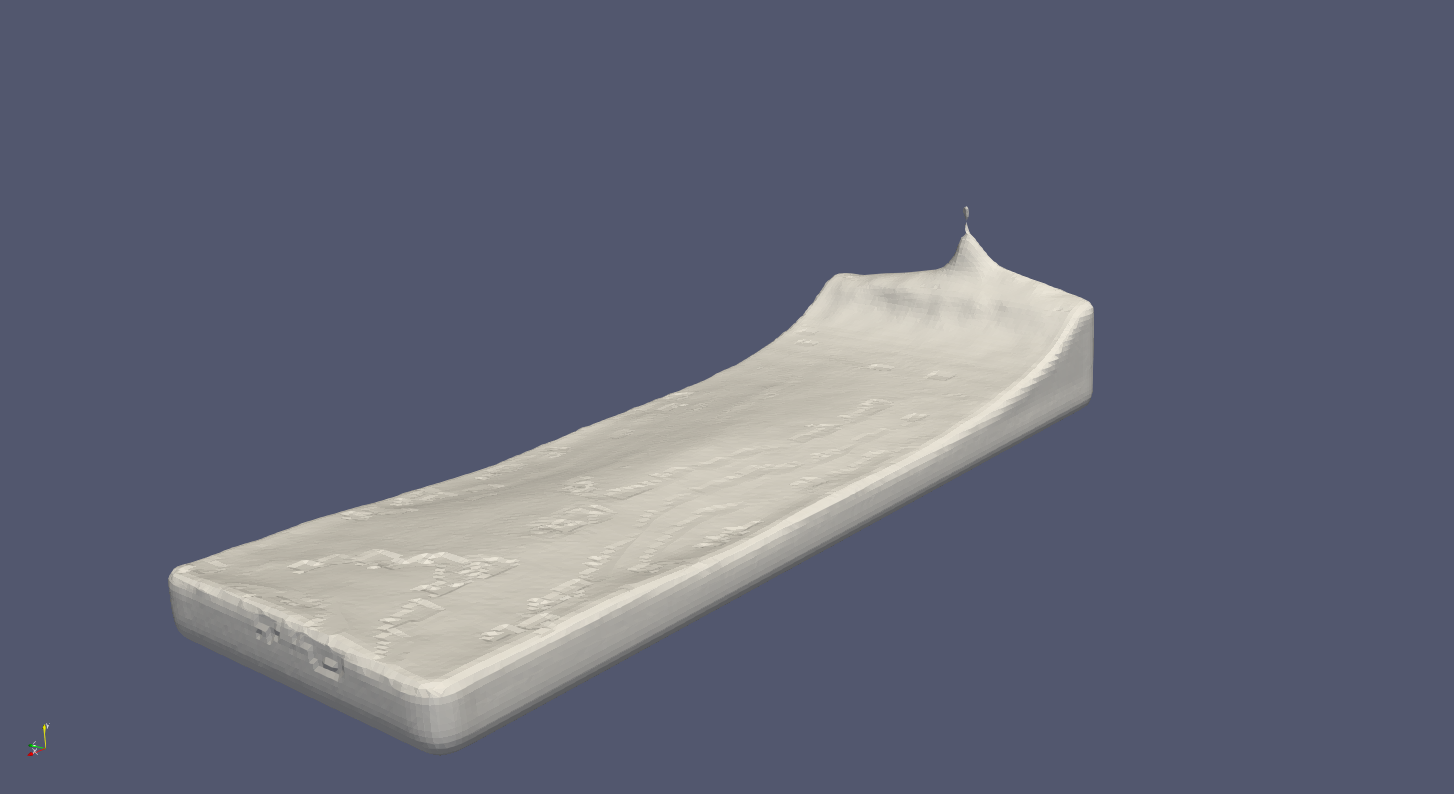
\includegraphics[width=\textwidth]{figures/KernelDepth1.png}
               \caption{Blur with full kernel size}
				\label{fig:kd_full}
        \end{subfigure}
        \begin{subfigure}[b]{0.5\textwidth}
               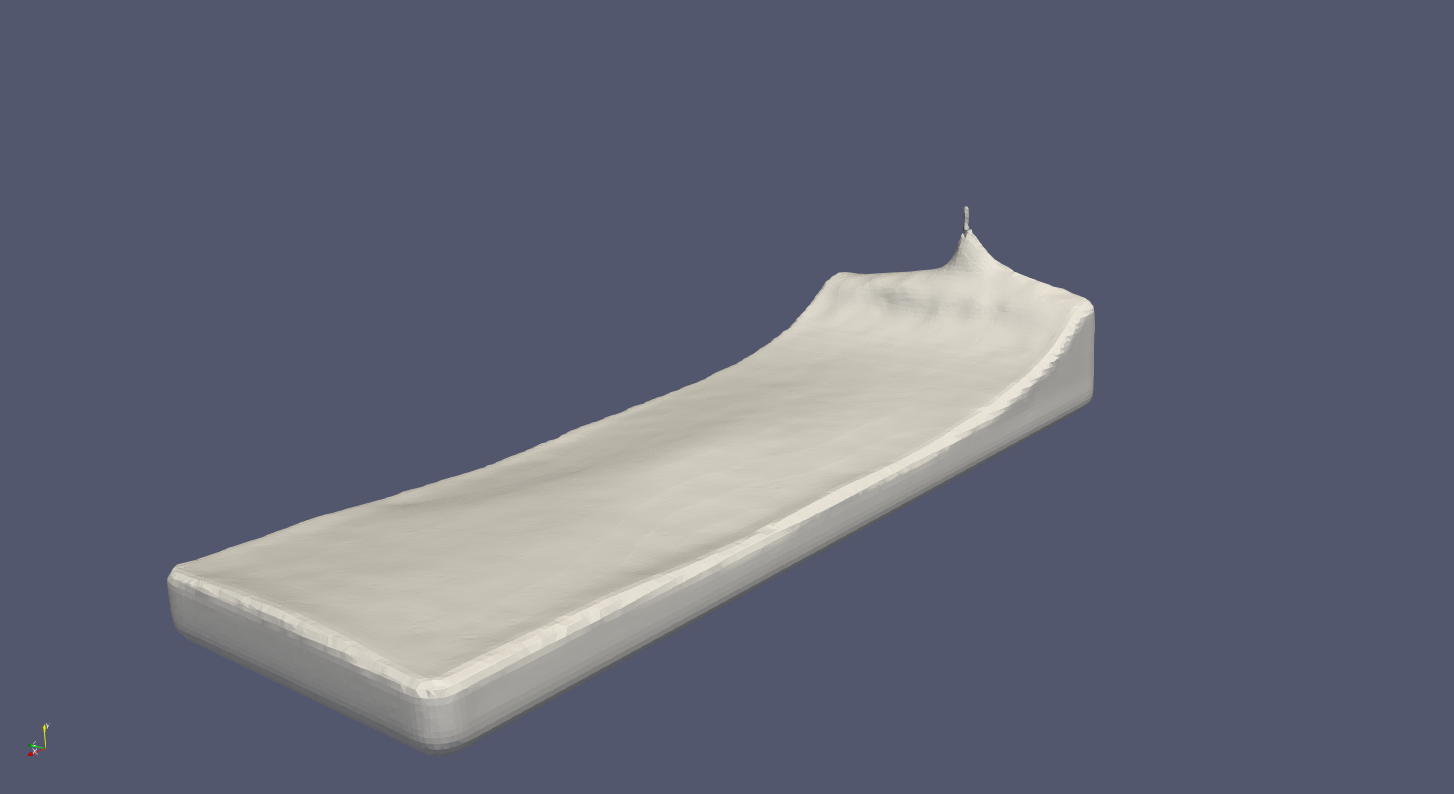
\includegraphics[width=\textwidth]{figures/KernelDepth0_5.png}
               \caption{Blur with half kernel size}
               \label{fig:kd_half}
        \end{subfigure}

       \caption{Influence of the kernel depth on level set blurring}
       \label{fig:kd_influence example}
 \end{figure}


\section{Blur Iterations}
Apart to other parameters it was decided to check the influence of application of blur iteratively to the level set. In the Algorithm \ref{alg:blur_alg} blur applied iteratively on the level set. The results of the iterative blur can be observed on the Figure \ref{fig:bi_reconstruction}. The higher number of blur iterations the smother resulting surface becomes. 
\begin{figure}[H]
        \begin{subfigure}[b]{0.5\textwidth}
               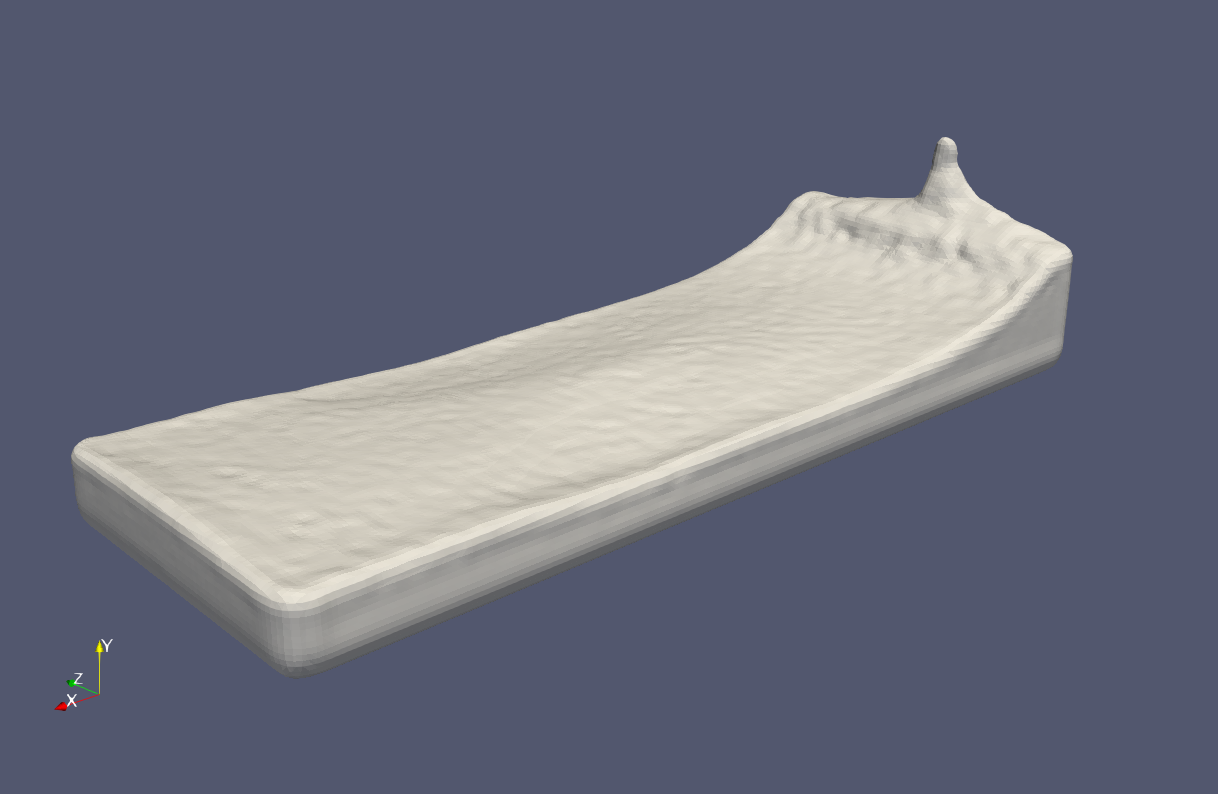
\includegraphics[width=\textwidth]{figures/ReconstructionIterations0.png}
				\caption{0 blur iterations}
               \label{fig:bi_original}
        \end{subfigure}
        \begin{subfigure}[b]{0.5\textwidth}
               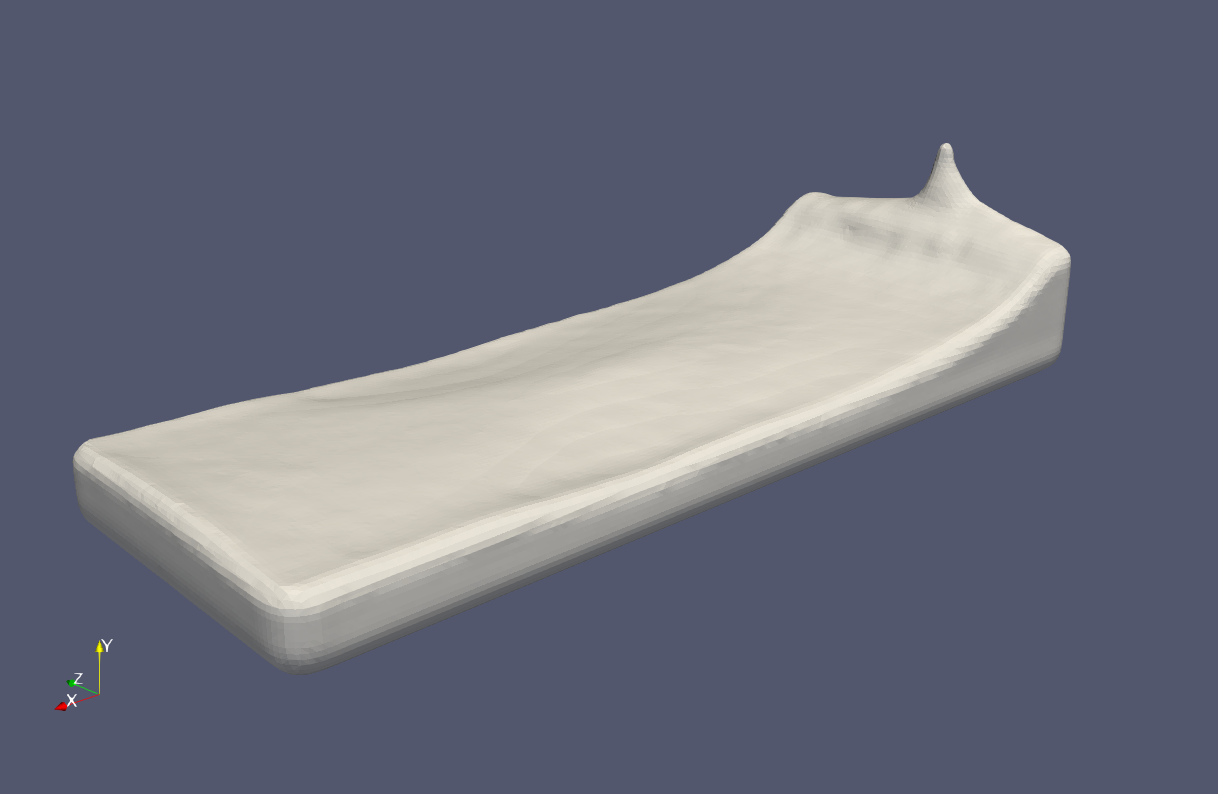
\includegraphics[width=\textwidth]{figures/ReconstructionIterations1.png}
				\caption{1 blur iterations}

				\label{fig:bi_1iteration}
        \end{subfigure}
        \begin{subfigure}[b]{0.5\textwidth}
               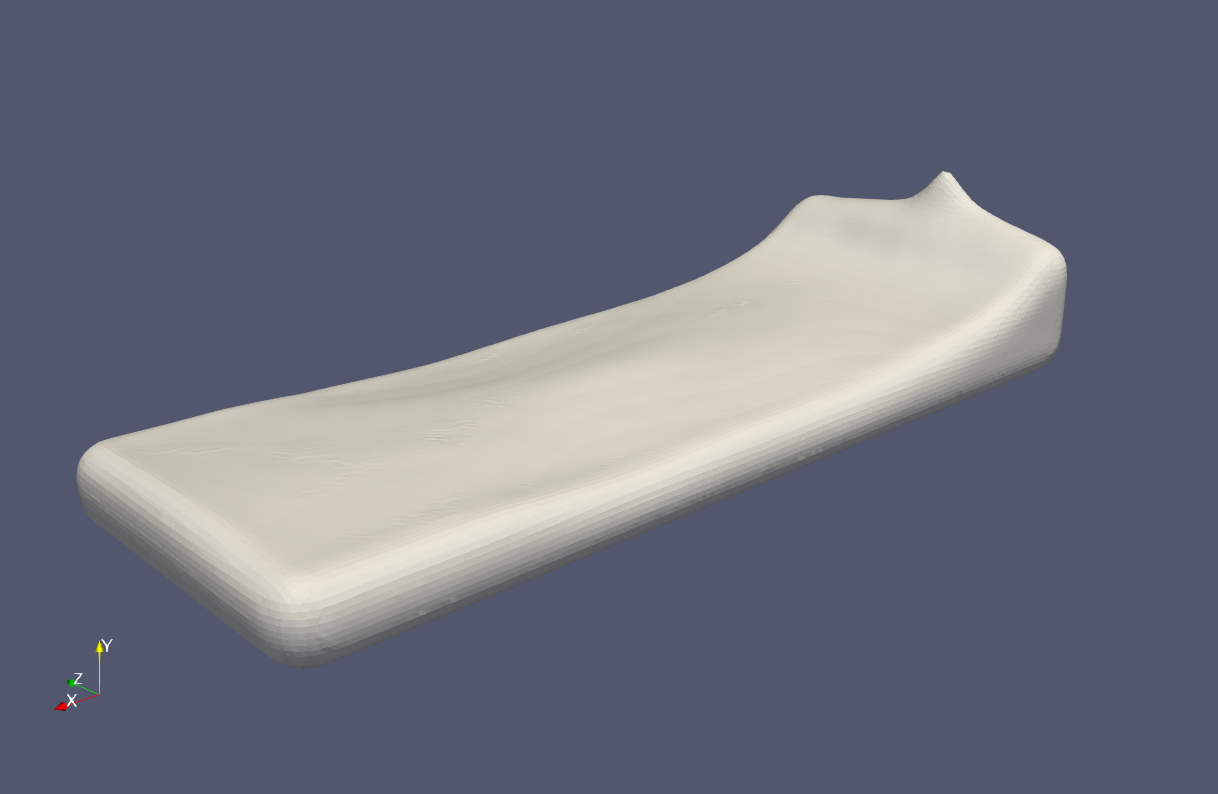
\includegraphics[width=\textwidth]{figures/ReconstructionIterations4.png}
				\caption{4 blur iterations}
               \label{fig:bi_4iteration}
        \end{subfigure}
        \begin{subfigure}[b]{0.5\textwidth}
               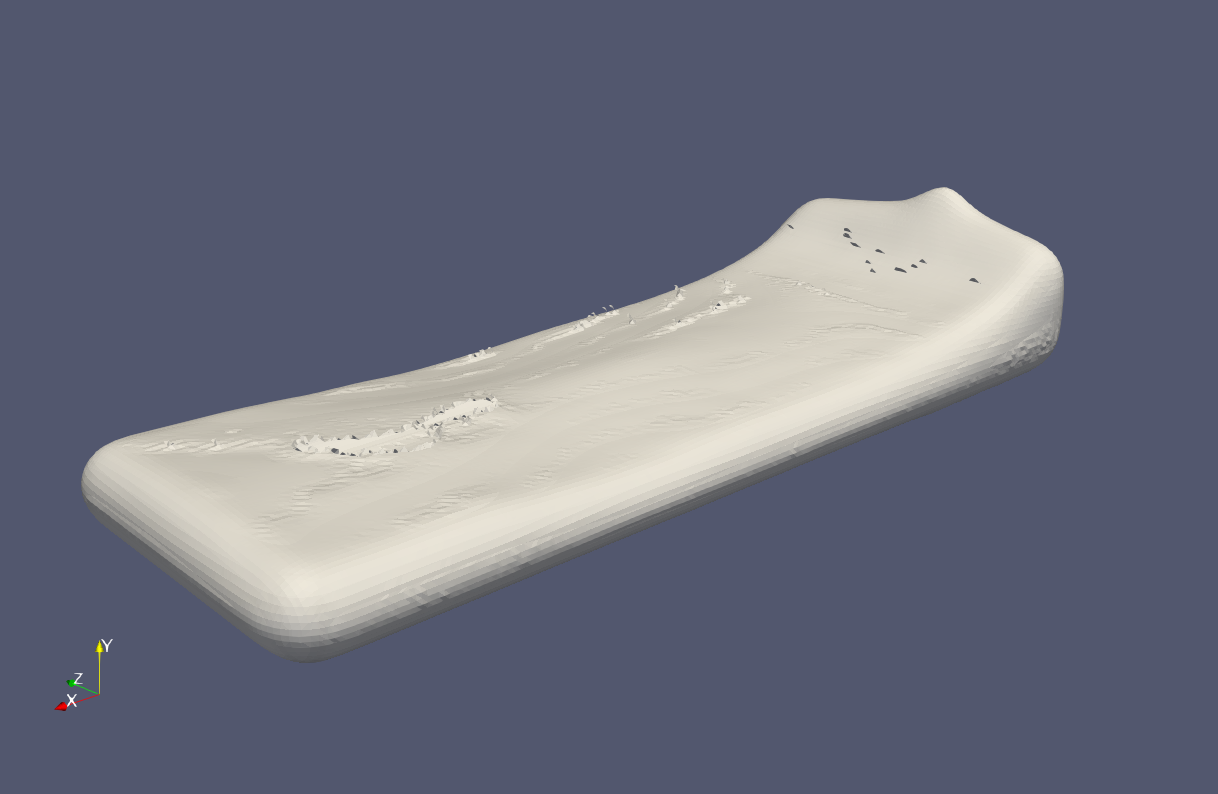
\includegraphics[width=\textwidth]{figures/ReconstructionIterations8.png}
				\caption{8 blur iterations}
               \label{fig:bi_8iteration}
        \end{subfigure}
       \caption{Reconstructed surface depending on the number of blur iterations}
       \label{fig:bi_reconstruction}
\end{figure}
However, large amount of iterations smooths out level set to uniform value, thus on the Figure \ref{fig:bi_8iteration} holes can be seen. Figure \ref{fig:bi_levelset} displays the influence of blur iterations on level set itself. 
\begin{figure}[H]
        \begin{subfigure}[b]{0.5\textwidth}
               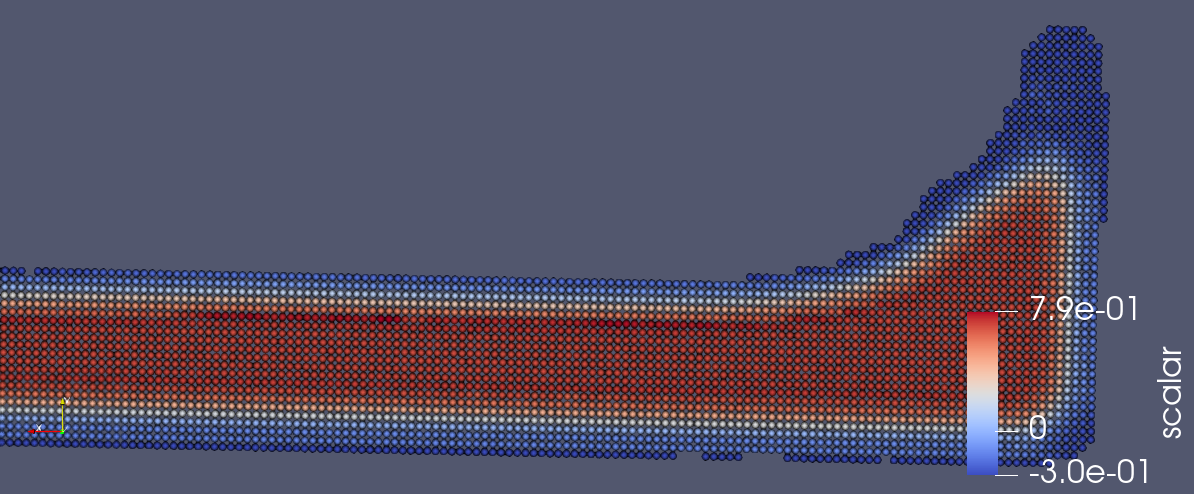
\includegraphics[width=\textwidth]{figures/LevelSetBlurIterations4.png}
				\caption{4 blur iterations}
               \label{fig:ls_bi_original}
        \end{subfigure}
        \begin{subfigure}[b]{0.5\textwidth}
               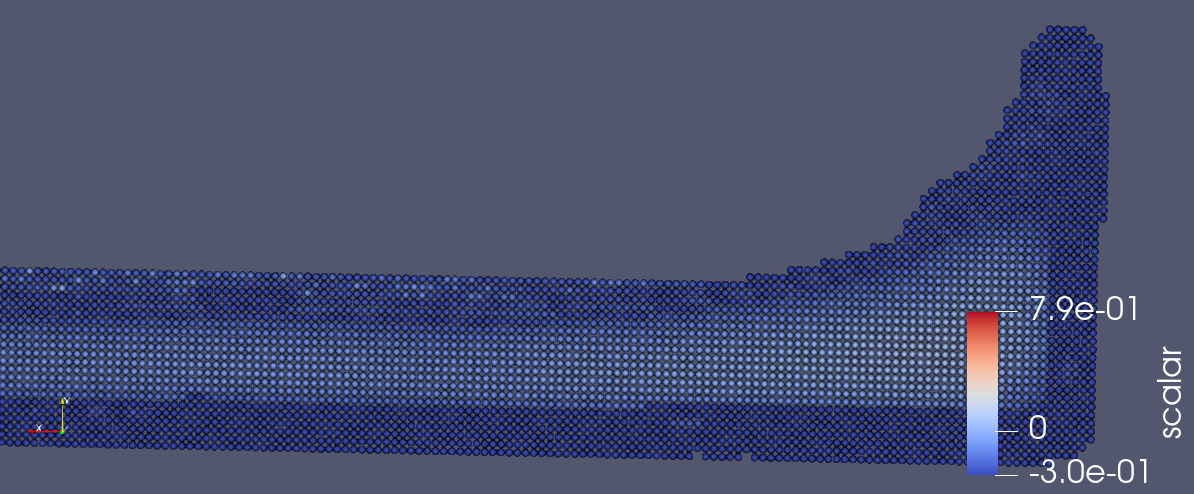
\includegraphics[width=\textwidth]{figures/LevelSetBlurIterations16.png}
				\caption{16 blur iterations}

				\label{fig:ls_bi_16iteration}
        \end{subfigure}
       \caption{Level set depending on the number of blur iterations}
       \label{fig:bi_levelset}
\end{figure}

An important property of the blur reconstruction algorithm should be noted. Lets analyze the blur algorithm, applied on the level set (for simplicity 2D version will be analyzed).\\
Suppose matrix $A = 
\begin{pmatrix}
	1 & 1 & ... & 1\\
	1 & 1 & ... & 1\\
	. & . & ... & .\\
	1 & 1 & ... & 1\\
\end{pmatrix}$ is a $n \times n$ kernel where n is odd.
Kernel multiplication operation on level set element is described in equation \ref{eq:kernel-operation}
\begin{equation}
	\dfrac{1}{n^2}\cdot A\cdot sdf_{ij} = \sum_{k=- \left \lfloor{n/2}\right \rfloor}^{\left \lfloor{n/2}\right \rfloor}
		{\sum_{l=- \left \lfloor{n/2}\right \rfloor}^{\left \lfloor{n/2}\right \rfloor}{ A_{k+1, l+1} \cdot sdf_{i+k, j+l}}}
	\label{eq:kernel-operation}
\end{equation}
Suppose $n=3$ and $ sdf^{(k)}_{i,j} = \dfrac{1}{9} \cdot A \cdot sdf^{(k-1)}_{i,j} = \dfrac{1}{9^k} \cdot A^{(k)} \cdot sdf^{(0)}_{i,j}$\\. The claim is that $\dfrac{A^{(k)}}{9^k}$ satisfies properties of a kernel function:
\begin{itemize}
	\item positivity condition : $\forall a_{ij} \in A^(k): a_{ij} >= 0$
	\item normalization condition: $\forall a_{ij} \in A^(k), i,j \in [n]: \dfrac{\sum{a_{ij}}}{9^k} = 1$
	\item symmetry condition: $\forall i,j k=\left \lfloor{\dfrac{n}{2}}\right \rfloor $
\end{itemize}
Thus, when applied to the MC vertices plays a role of weights of the level set values in the neighborhood of the central vertice.\\
Proof of positivity condition:\\
As soon as each element of $A^{(k)}$ is formed by summing up neighboring elements of $A^{(k-1)}$ that is $a_{ij}^{(k)} = \sum_{k=-1}^{1}{\sum_{l=-1}^{1}{a^{(k-1)}_{i+k, j+l}}}$, then by simple induction starting with initial kernel $A^(1)=
\begin{pmatrix}
1 & 1 & 1\\
1 & 1 & 1\\
1 & 1 & 1\\
\end{pmatrix}$
it can be proven, that $a_{ij}^{(k)} >= a_{ij}^{(k-1)} >= a_{ij}^{(1)}$.\\
Proof of normalization condition: \\
Base step:\\ 
For initial matrix $A^{(1)}$ it is obvious that $\dfrac{\sum_{i,j = 1}^{n}{a_{ij}}}{9} = 1$.\\
Induction step: \\
Let $\dfrac{A^{(k)}}{9^k} = 1$. Taking into account, that $a_{ij}^{(k+1)} = \sum_{k=-1}^{1}{\sum_{l=-1}^{1}{a^{(k)}_{i+k, j+l}}}$ then $\forall a_{ij} \in A^{(k)}$ will appear in the sum of elements of $A^{(k+1)}$ exactly 9 times. Thus $\sum_{i,j}{a_{ij}^{(k+1)}} = 9 \cdot \sum_{i,j}{a_{ij}^{(k)}} = 9^{k+1}$\\
Some examples of a kernel functions iteratively formed from uniform kernel with kernel size = 1:\\
$A^2 = 
\begin{pmatrix}
1 & 2 & 3 & 2 & 1\\
2 & 4 & 6 & 4 & 2\\
3 & 6 & 9 & 6 & 3\\
2 & 4 & 6 & 4 & 2\\
1 & 2 & 3 & 2 & 1\\
\end{pmatrix}$
$A^3 = 
\begin{pmatrix}
 1 & 3 & 6 & 7 & 6 & 3 & 1\\
 3 & 9 & 18 & 21 & 18 & 9 & 3\\
 6 & 18 & 36 & 42 & 36 & 18 & 6\\
 7 & 21 & 42 & 49 & 42 & 21 & 7\\
 6 & 18 & 36 & 42 & 36 & 18 & 6\\
 3 & 9 & 18 & 21 & 18 & 9 & 3\\
 1 & 3 & 6 & 7 & 6 & 3 & 1\\
\end{pmatrix}$\\
$A^4 = 
\begin{pmatrix}
1 & 4 & 10 & 16 & 19 & 16 & 10 & 4 & 1\\
4 & 16 & 40 & 64 & 76 & 64 & 40 & 16 & 4\\
10 & 40 & 100 & 160 & 190 & 160 & 100 & 40 & 10\\
16 & 64 & 160 & 256 & 304 & 256 & 160 & 64 & 16\\
19 & 76 & 190 & 304 & 361 & 304 & 190 & 76 & 19\\
16 & 64 & 160 & 256 & 304 & 256 & 160 & 64 & 16\\
10 & 40 & 100 & 160 & 190 & 160 & 100 & 40 & 10\\
4 & 16 & 40 & 64 & 76 & 64 & 40 & 16 & 4\\
1 & 4 & 10 & 16 & 19 & 16 & 10 & 4 & 1\\
\end{pmatrix}$\\
This means, that given a kernel size = 1, kernel offset = 0 and blur iterations = n the final blur kernel applied will have a form of $ n \times n$ kernel that satisfies the kernel function conditions (proof for 3D case is similar for 2D case). Also the cost of the blur stage is reduced from $O(p \cdot n^2)$ when using $n \times n$ kernel to $O(9 \cdot p \cdot n)$ when using $3\times 3$ kernel applied n times on p MC grid cells. However, in  case of iterative approach kernel converges to Gaussian, in the latter case uniform kernel is applied. 


\section{Results and Performance comparison}
In this section performance of the blur algorithm will be analyzed w.r.t. the original reconstruction methods. All tests was performed on one core of AMD Ryzen 5. No parallelization was applied simplify the analysis.
Table \ref{tab:perf_analysis} shows the wall-clock time for each method in different stages.
Reconstruction was performed on the simulation with 40000 particles, 93 frames and 0.02 particle radius, where:
\begin{conditions}
	DB & Density based reconstruction (MC grid resolution: 0.020000)\\
	DBblur & Density based reconstruction with level set blur (Kernel size: 2, Kernel offset: 1, Kernel depth: 0.5, Blur iterations: 1)\\
	ZB & Zhu and Bridson reconstruction (MC grid resolution: 0.020000, Support radius: 0.08\\
	ZBblur & Zhu and Bridson with level set blur (Smoothing factor: 1, Kernel size: 2, Kernel offset: 1, Kernel depth: 0.5, Blur iterations: 1)\\
\end{conditions}
\begin{table}[h]
	\begin{center}
		\scriptsize
		\begin{tabular}{|l|c|c|c|c|c|c|}
			\hline
			Simulation type & DB & DBblur & ZB & ZBblur \\
			\hline
			Total execution time		&	250.210204	&	362.309801	&	227.907790	&	339.686174	\\
			Hash tables update			&	1.292020	&	1.491784	&	1.846468	&	2.009707	\\
			Detect surface particles	&	12.742551	&	12.753376	&	12.821589	&	12.805908	\\
			MC grid update				&	109.401044	&	108.327551	&	66.569929	&	68.213688	\\
			Level set update			&	113.503782	&	226.926150	&	125.736858	&	245.192591	\\
			Mesh generation				&	11.154644	&	10.985956	&	17.596987	&	9.521316	\\
			\hline
		\end{tabular}
	\end{center}
	\caption{Per stage performance analysis of original reconstruction methods versus level set blur}
	\label{tab:perf_analysis}
\end{table}

In Table \ref{tab:ks_perf_analysis} performance of the application is analyzed depending on the kernel size. Static simulation parameters:
\begin{conditions}
	\text{particle count}  & 40000\\
	\text{particle radius} & 0.02\\
	\text{smoothing factor} & 1.0\\
	\text{kernel offset} & 1\\
	\text{kernel size} & 1\\
	\text{kernel depth} & 1.0\\
	\text{blur iterations} & 1\\
\end{conditions}
\begin{table}[H]
	\begin{center}
		\scriptsize
		\begin{tabular}{|l|c|c|c|c|c|c|}
			\hline
			Kernel size & 1 & 2 & 3 & 4 \\
			\hline
			Hash tables update (sec)		&	0.036016	&	0.035996	&	0.036947	&	0.034786	\\
			Mesh generation	(sec)			&	0.154370	&	0.155268	&	0.154680	&	0.155067	\\
			Total execution time (sec)		&	4.661093	&	5.880080	&	8.681242	&	14.524655	\\
			MC grid update (sec)			&	1.350534	&	1.414452	&	1.378100	&	1.463115	\\
			Level set update (sec)			&	2.721548	&	3.873281	&	6.716356	&	12.471516	\\
			Detect surface particles(sec)	&	0.273974	&	0.274874	&	0.273340	&	0.276328	\\
			\hline
		\end{tabular}
	\end{center}
	\caption{Blur level set method performance depending on kernel size}
	\label{tab:ks_perf_analysis}
\end{table}
From Table \ref{tab:ks_perf_analysis} it can be seen, that the runtime of the level set reconstruction rises in a factor of kernel size.\\

In Table \ref{tab:bi_perf_analysis} reconstruction runtime is given for the blur reconstruction depending on the blur iterations. 
\begin{table}[H]
	\begin{center}
		\scriptsize
		\begin{tabular}{|l|c|c|c|c|c|c|c|}
			\hline
			Blur iterations & 0 & 1 & 2 & 3 & 4 \\
			\hline
			Hash tables update (sec)		&	0.030858	&	0.037154	&	0.034373	&	0.035957	&	0.034917\\
			Mesh generation	(sec)			&	0.151087	&	0.154440	&	0.154813	&	 0.153584	&	0.153664\\
			Total execution time (sec)		&	4.007258	&	4.708030	&	5.272999	&	5.839118	&	6.475744\\
			MC grid update (sec)			&	1.435496	&	1.377351	&	1.393668	&	1.391468	&	1.443232\\
			Level set update (sec)			&	1.968029	&	2.715168	&	3.295140	&	3.859314	&	4.445282\\
			Detect surface particles(sec)	&	0.278672	&	0.280408	&	0.273828	&	0.276087	&	0.278408\\
			\hline
		\end{tabular}
	\end{center}
	\caption{Blur level set method performance depending on blur iterations}
	\label{tab:bi_perf_analysis}
\end{table}
Runtime of the reconstruction depends linearly on the number of blur iterations.\\

Table \ref{tab:kd_perf_analysis} shows the performance of the application depending on the kernel depth value. Here kernel size is fixed to 5.
\begin{table}[H]
	\begin{center}
		\scriptsize
		\begin{tabular}{|l|c|c|c|c|}
			\hline
			Kernel depth & 0.1 & 0.25 & 0.5 & 1 \\
			\hline
			Hash tables update (sec)		&	0.035469	&	0.034264	&	0.035009	&	0.036902\\
			Mesh generation	(sec)			&	0.153513	&	0.153441	&	0.154675	&	 0.155028\\
			Total execution time (sec)		&	14.684650	&	16.564669	&	19.218910	&	24.861456\\
			MC grid update (sec)			&	1.427892	&	1.379971	&	1.413553	&	1.435164\\
			Level set update (sec)			&	12.667619	&	14.592833	&	17.217208	&	22.836116\\
			Detect surface particles(sec)	&	0.276308	&	0.281181	&	0.272071	&	0.276914\\
			\hline
		\end{tabular}
	\end{center}
	\caption{Blur level set method performance depending on kernel depth}
	\label{tab:kd_perf_analysis}
\end{table}

Figure \ref{fig:DamBreak} displays the  the comparison of reconstruction results between original method and applied blur.
\begin{figure}[h]
	\begin{center}
        \begin{subfigure}[b]{0.4\textwidth}
               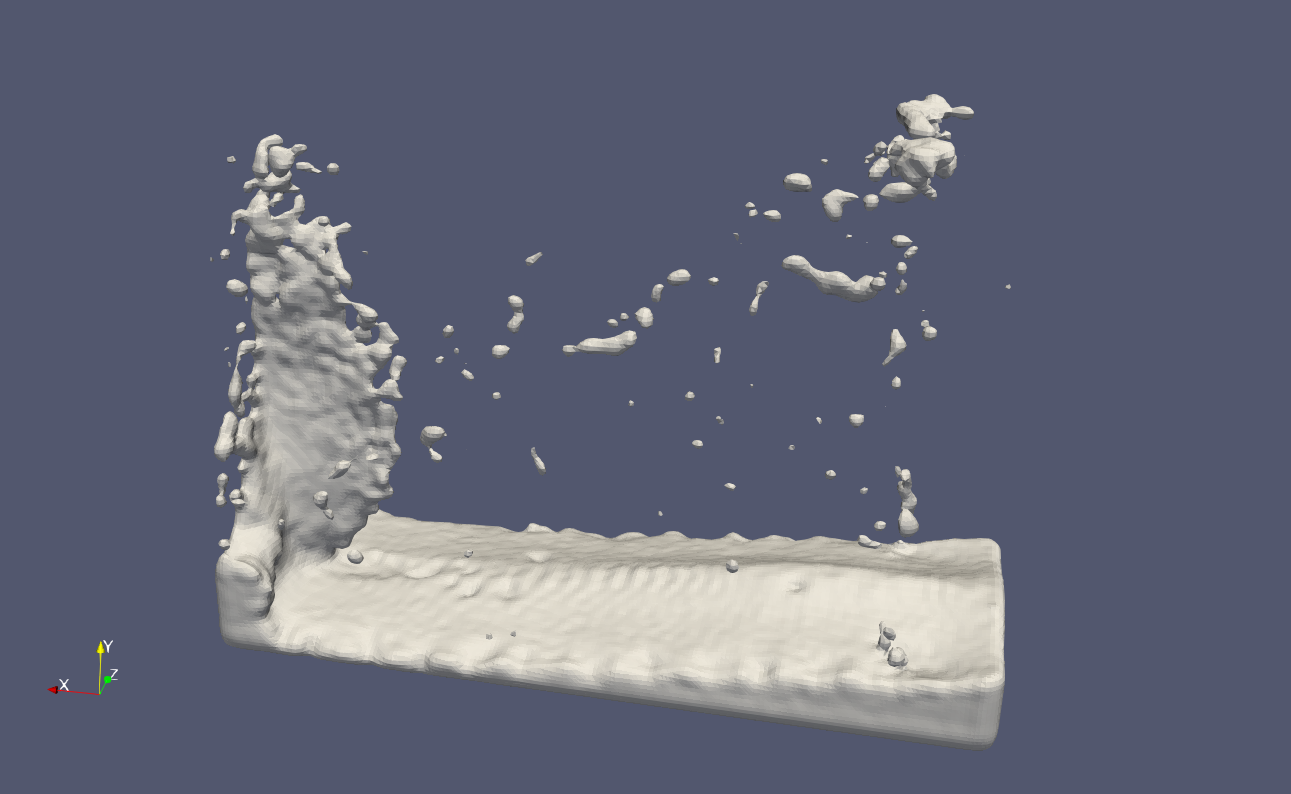
\includegraphics[width=\textwidth]{figures/ReconstructionDencityBased.png}
				\caption{Method: DB}
        \end{subfigure}
        \begin{subfigure}[b]{0.4\textwidth}
               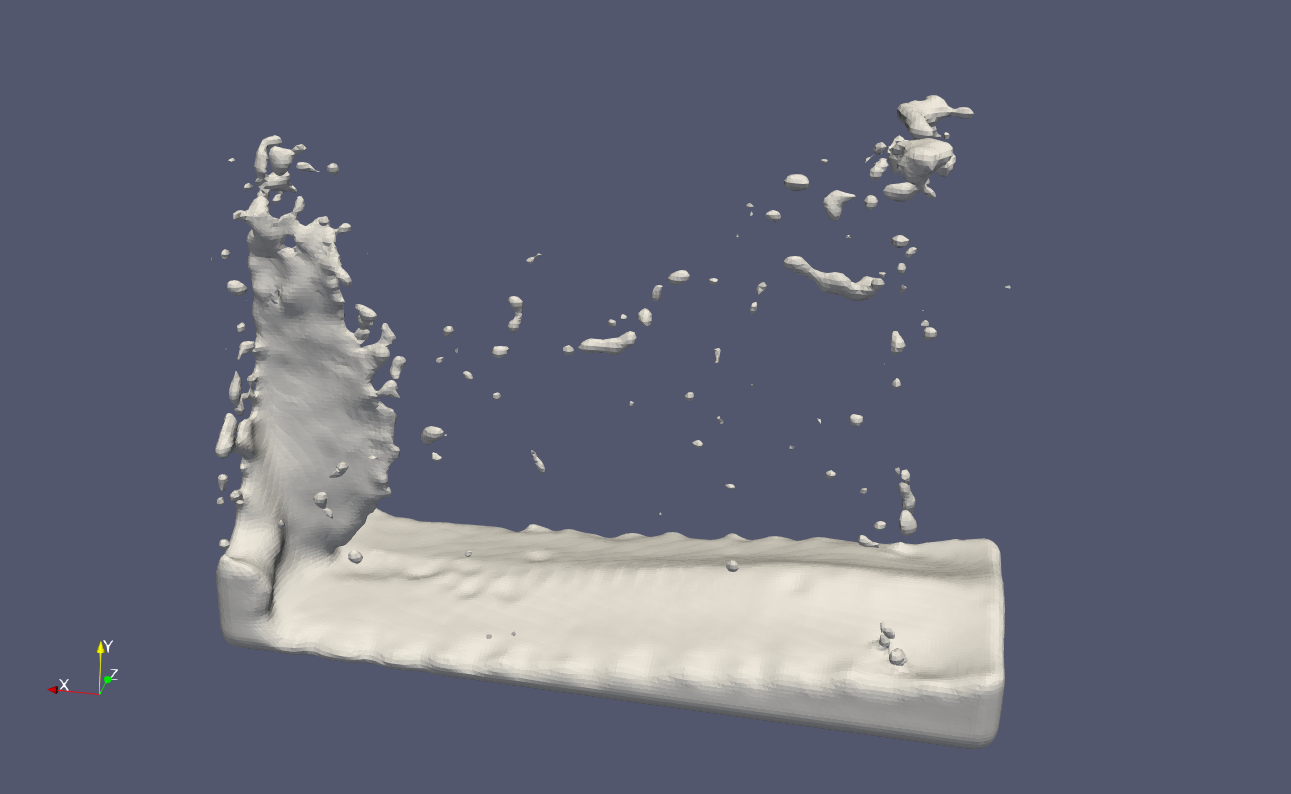
\includegraphics[width=\textwidth]{figures/ReconstructionDencityBasedBlur.png}
				\caption{Method: DBblur}
        \end{subfigure}
        \begin{subfigure}[b]{0.4\textwidth}
               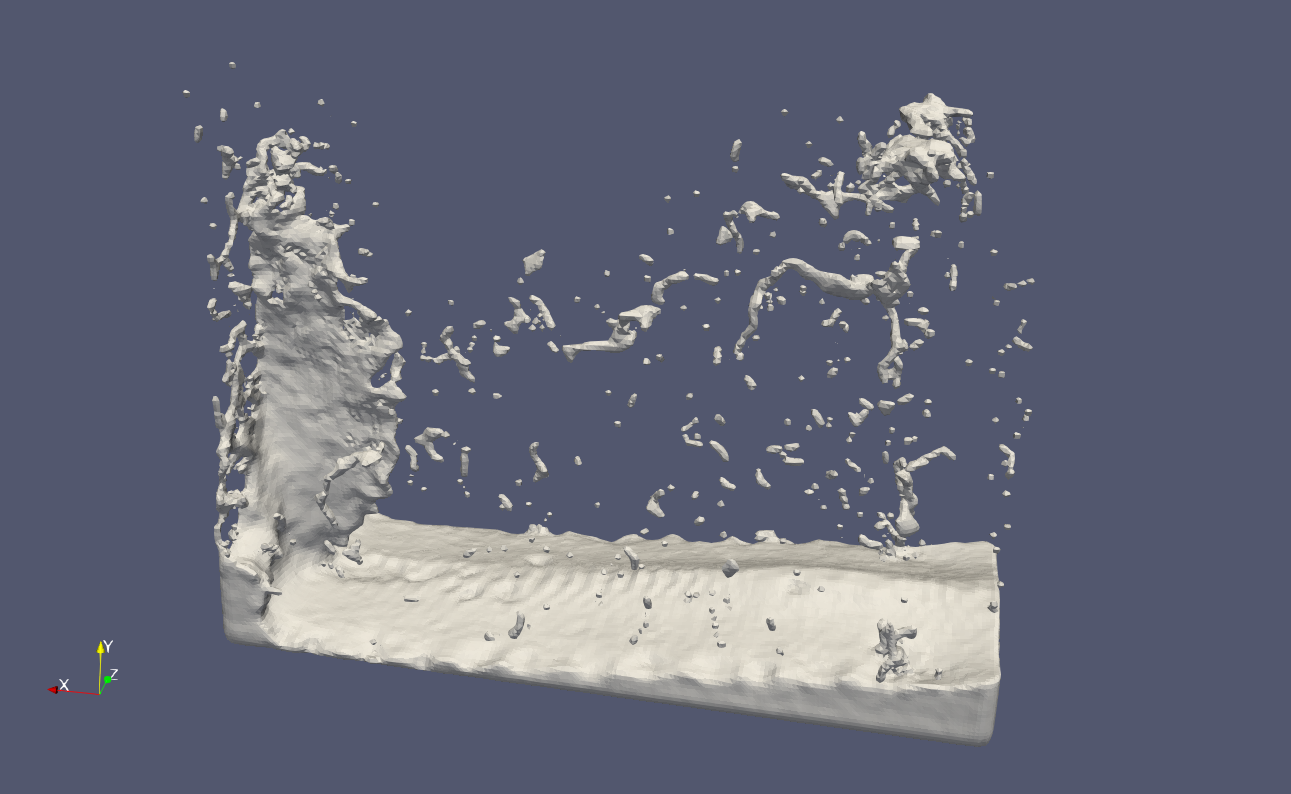
\includegraphics[width=\textwidth]{figures/ReconstructionZhuBridson.png}
				\caption{Method: ZB}
        \end{subfigure}
        \begin{subfigure}[b]{0.4\textwidth}
               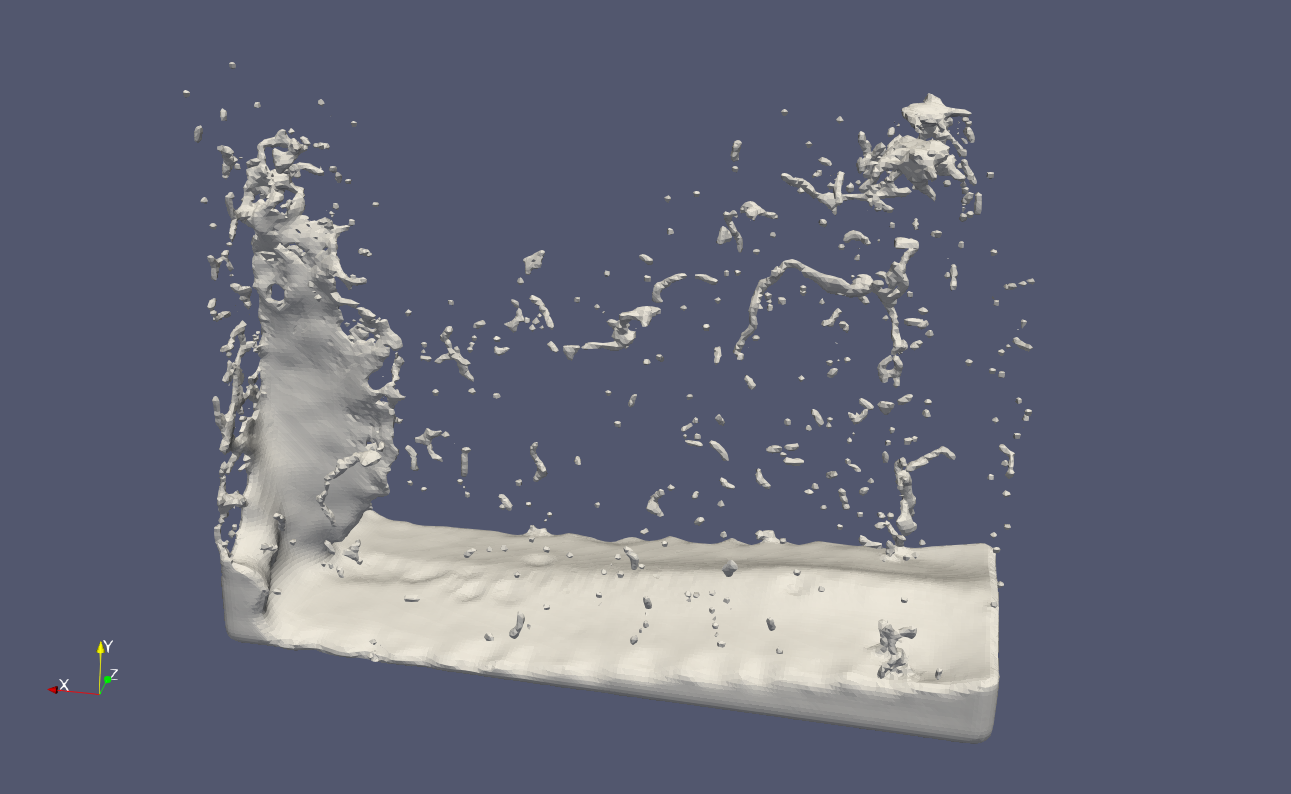
\includegraphics[width=\textwidth]{figures/ReconstructionZhuBridsonBlur.png}
				\caption{Method: ZBblur}
        \end{subfigure}
        \caption{Fluid surface comparison in dam break scene}
        \label{fig:DamBreak}
	\end{center}
\end{figure}


Another scene comparison is shown in the figure \ref{fig:MotorScene}. Particle count - 5000, particle radius - 0.025
\begin{figure}[h]
	\begin{center}
        \begin{subfigure}[b]{0.4\textwidth}
               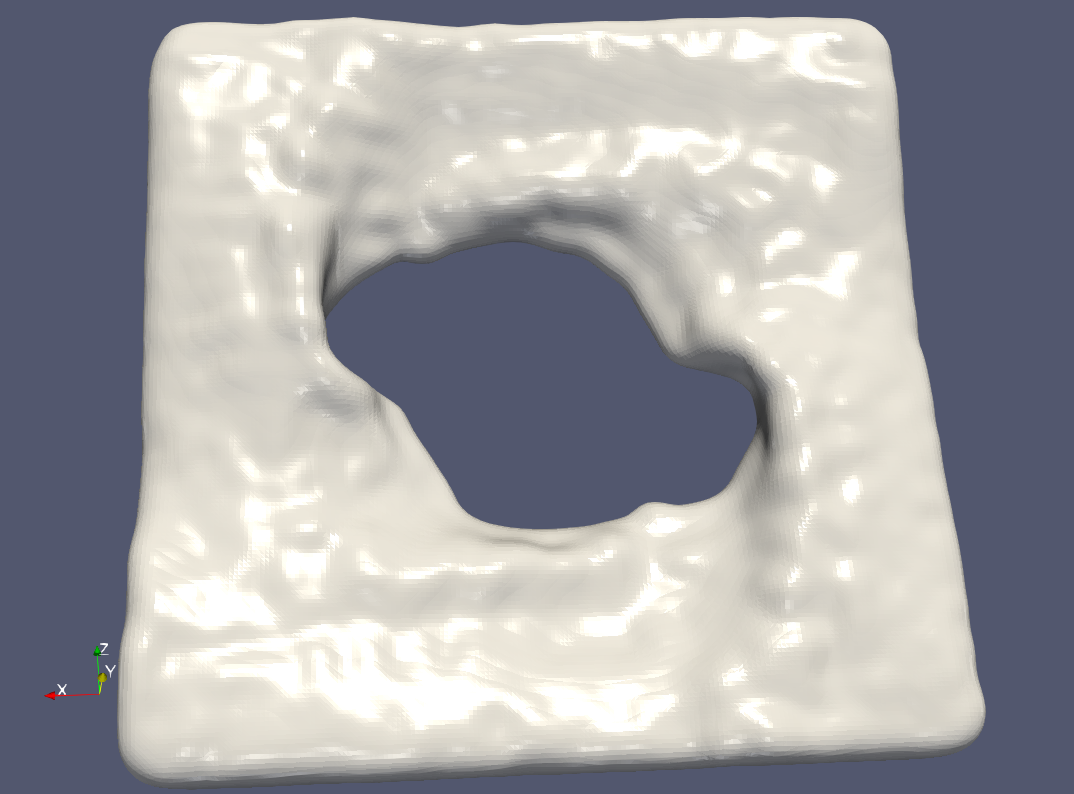
\includegraphics[width=\textwidth]{figures/ReconstructionMotorSceneDencityBased.png}
				\caption{Method: DB}
        \end{subfigure}
        \begin{subfigure}[b]{0.4\textwidth}
               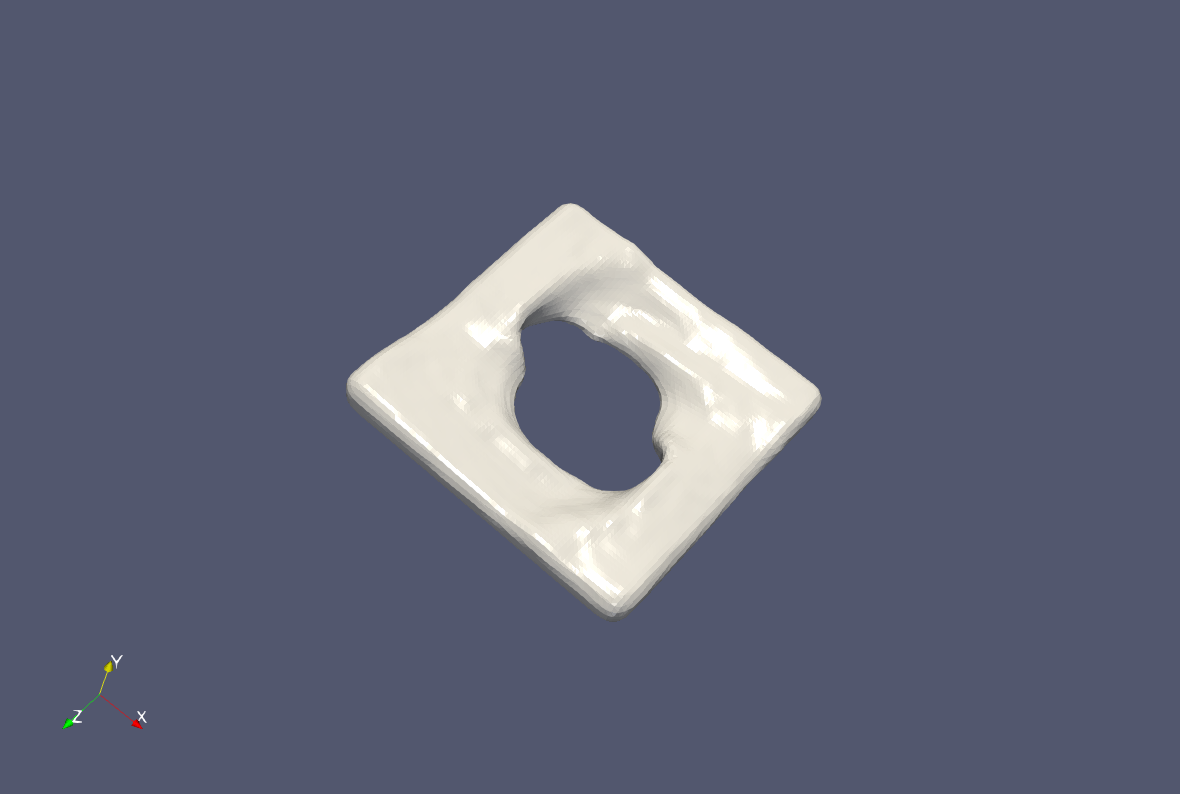
\includegraphics[width=\textwidth]{figures/ReconstructionMotorSceneDencityBasedBlur.png}
				\caption{Method: DBblur}
        \end{subfigure}
        \begin{subfigure}[b]{0.4\textwidth}
               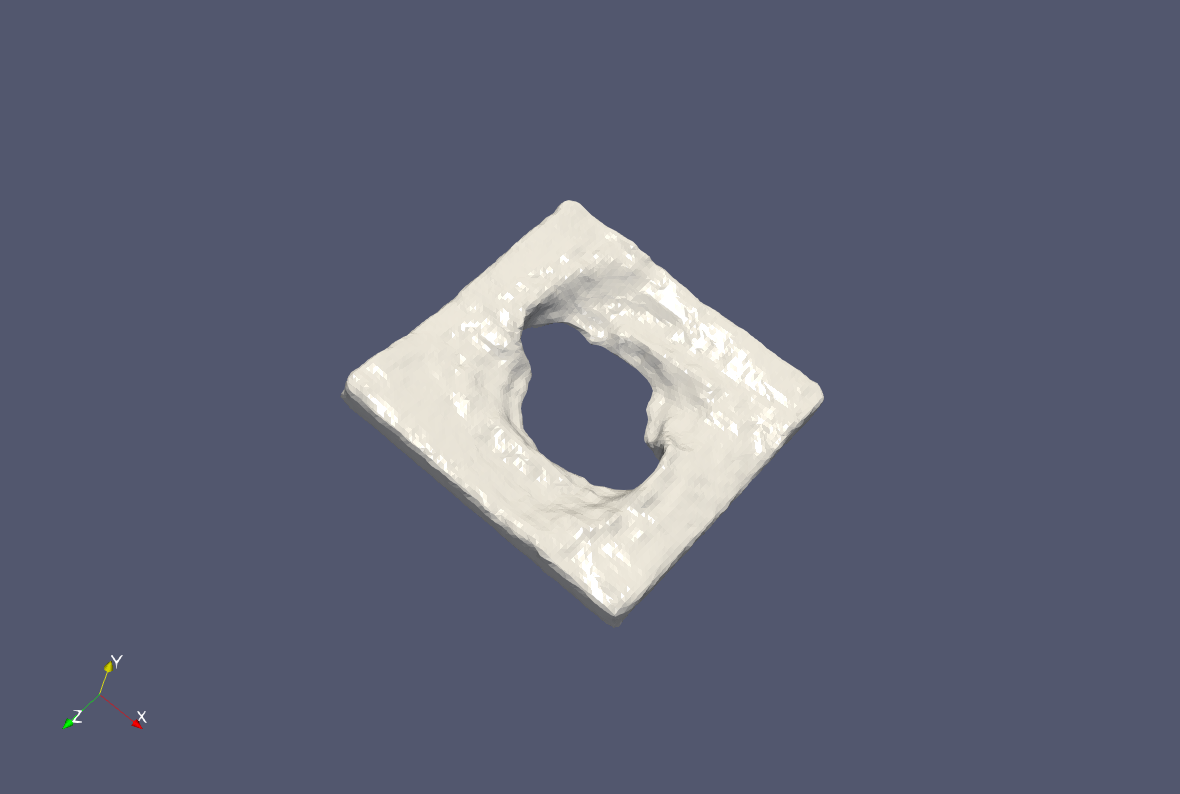
\includegraphics[width=\textwidth]{figures/ReconstructionMotorSceneZhuBridson.png}
				\caption{Method: ZB}
        \end{subfigure}
        \begin{subfigure}[b]{0.4\textwidth}
               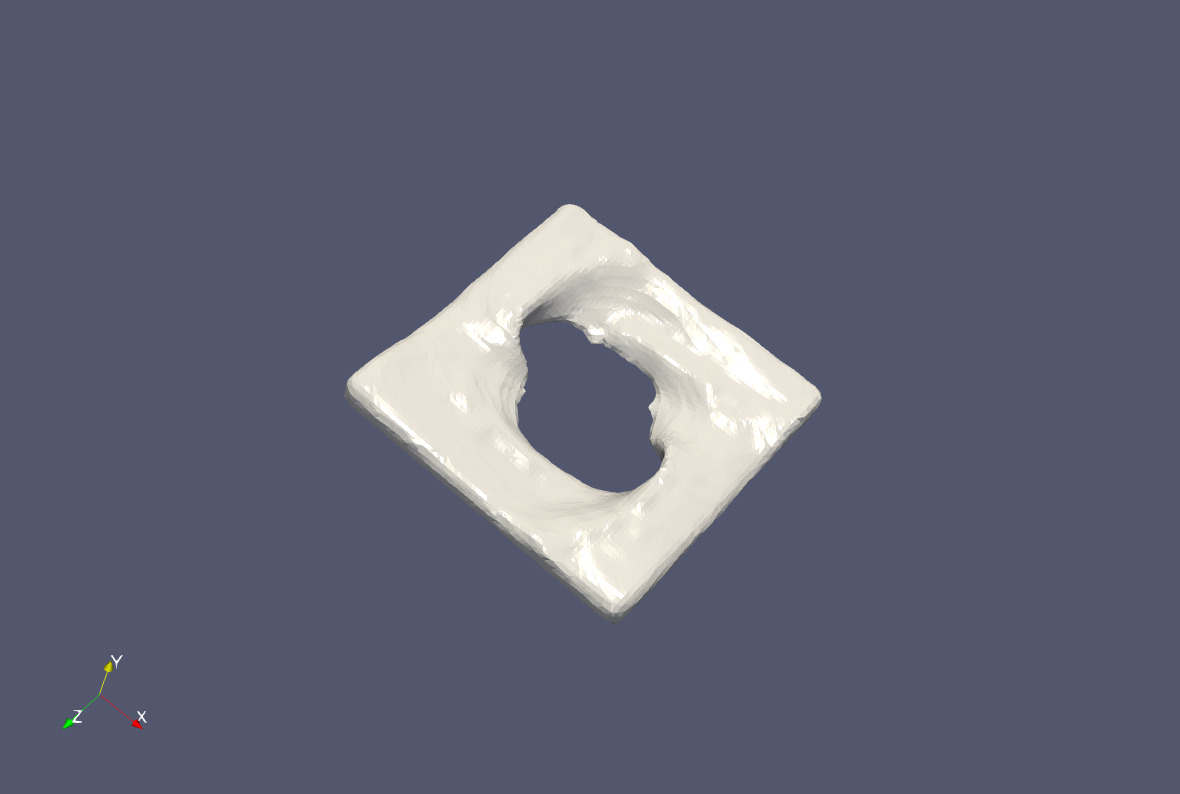
\includegraphics[width=\textwidth]{figures/ReconstructionMotorSceneZhuBridsonBlur.png}
				\caption{Method: ZBblur}
        \end{subfigure}
        \caption{Motor scene fluid surface reconstruction comparison}
        \label{fig:MotorScene}
	\end{center}
\end{figure}



\section{Conclusions}
After performing previously described experimentations with the developed method the conclusion can be made, that application of blur to the level set is definitely influences the final surface quality, and this method is able to smooth flat areas of surface, in the mean time saving small features in splash areas. The developed algorithm is applied on top of the original reconstruction algorithm. It can be applied to every reconstruction method, which uses scalar distance field to construct iso-surfaces and reconstruct the surface itself.\\ 
In the future efforts can be applied to improve algorithm performance, e.g. porting blur stage on GPU. The blur stage of the algorithm.\\
However, this method still has severe drawback - a problem of parametrization. There are multiple parameters that should be tunned, such as kernel size, kernel offset, kernel depth, smoothing factor, blur iterations. For different reconstruction methods, depending on the structure of the level set, simulation scale, performance and surface quality requirements, there is no golden middle for automatic application of the parametrization. Thus manual parameters tuning is required to achieve required reconstruction quality.\\
Two approach can be used to define a parametrization - fix kernel size = 1, kernel offset = 0, kernel depth = 1 and modify number of blur iterations and smoothing factor. In this case performance will be improved, but blur will not be flexible to the near surface areas, thus sharp features could be smoothed too much.\\
Another approach is to modify kernel size, kernel depth and smoothing factor, while keeping blur iterations fixed to 1. In this case most reconstruction method is more flexible to blurring low frequency bumps in flat surface areas saving most of the sharp features, meanwhile the performance of the reconstruction will be degraded.


\chapter{Moving least squares level set smoothing}
\section{Introduction}
As were previously concluded blur level set method requires hight effort to configure all available parameters to match required fluid surface reconstruction quality. Another helpful method comes in mind, which can be applied to correct an implicit ISO-surface such, that the explicit reconstructed surface will be smoothed out.\\
Moving Least Squares (MLS) is a method for recovering continuous functions from a set of random point samples by calculating a weighted least squares measure biased toward the area around the point at which the retrieved value is requested. Holding in mind, that scalar distance field is the implicit function of the distance to surface, it can be assumed that in the small local neighborhood the function should fit an elementary surface e.g. sphere.\\
In the work \cite{Apss} new Point Set Surface (PSS) definition based on moving least squares (MLS) fitting of algebraic spheres is presented. The central advantages of APSS approach compared to existing planar MLS include significantly improved stability of the projection under low sampling rates and in the presence of high curvature. \textcolor{red}{TODO: add more descriptions}\\
Another important work was performed in \cite{PssLkr} \textcolor{red}{TODO: add description of the work}.\\
In this thesis MLS was applied directly on the SDF. As a blur level set method the level set mls correction method is also developed to be able to apply it on every reconstruction approach, which in the core uses an implicit SDF ISO-surface.  
\section{Moving least squares}
In this section concept of the Moving Least Squares (MLS) will be described. The MLS approximation was introduced in an early paper by Lancaster and Salkauskas  \cite{MLSSalkauskas} in 1981 with special cases going back to McLain  \cite{MLSMcLain1}, \cite{MLSMcLain2} in 1974 and 1976. Since, in MLS one writes the value of the unknown function in terms of scattered data, it can be used as an approximation to span the trial space in meshless (or meshfree) methods. This approximation has found many applications in curve fitting and numerical solutions of partial differential equations.\\
Most of the theoretical material was taken from \cite{MLSIntro}.
\subsection{Global least squares}
\textbf{Problem domain.} Given a points $X = [x_1, ..., x_n]$. The goal of a is to fit point cloud to some geometric surface e.g. sphere. Suppose, that we are given a values of $u(X) = [u_1, ..., u_n]$ and the values are biased, e.g. $u_i + \varepsilon = u(x_i)$ and the function $u(x)$ is unknown.\\ 
The idea of a Global Least Squares (GLS) technique is to reconstruct $u(x)$ so that for all $|u_i - u(x_i)|$ is minimal, that is:
\begin{equation}
	\sum_i (u_i - u(x_i))^2 -> min
	\label{eq:min_problem}
\end{equation}
\textbf{Description.} For simplicity 1D problem will be reviewed e.g. $x_i \in R$. Function $u(x_i)$ can be described as polynomial $u(x)=\sum_k{c_i \cdot x^k}$, where $c_i$ are unknown coefficients, which are to be found.
As soon as in the problem domain $x_i$ are given values we can substitute a $x^k$ with a coefficient $b_k(x) = x^k$. Returning to the equation \ref{eq:min_problem} no the equation can be expanded the minimization problem:
\begin{equation}
	\sum_i (u_i - \sum_j{c_j \cdot b_j(x_i)})^2 = R^{GLS}
	\label{eq:min_problem_exp}
\end{equation}
where $R^{GLS}$ is a function to be minimized. Finding a minimum first derivative of the equation \ref{eq:min_problem_exp} w.r.t. $c_j$ should be taken, and assigned to 0. An example of one derivative over $c_k$ is in Equation \ref{eq:RGLSderivatieve}
\begin{equation}
	\dfrac{\partial R^{GLS}}{\partial c_k} = 2\cdot \sum_i{b_k(x_i) \cdot (\sum_j{b_j(x_i)\cdot c_j} - u_i)} = 0
	\label{eq:RGLSderivatieve}
\end{equation}
or equation \ref{eq:RGLSderivatieve}  can be rewritten as follows:
\begin{equation}
	\sum_i{b_k(x_i) \cdot (\sum_j{b_j(x_i)\cdot c_j})}  = \sum_i {b_k(x_i) \cdot u_i}
	\label{eq:RGLSderFinal}
\end{equation}
Taking all partial derivatives over $c_j$ the set of equations can be generated $LS = 
\begin{matrix}
	\sum_i{b_1(x_i) \cdot (\sum_j{b_j(x_i)\cdot c_j})}  &= \sum_i {b_1(x_i) \cdot u_i}\\
	\sum_i{b_2(x_i) \cdot (\sum_j{b_j(x_i)\cdot c_j})}  &= \sum_i {b_2(x_i) \cdot u_i}\\
	\sum_i{b_3(x_i) \cdot (\sum_j{b_j(x_i)\cdot c_j})}  &= \sum_i {b_3(x_i) \cdot u_i}\\
	...\\
	\sum_i{b_m(x_i) \cdot (\sum_j{b_j(x_i)\cdot c_j})}  &= \sum_i {b_m(x_i) \cdot u_i}\\
\end{matrix}$\\
This is a linear system with m equations and m unknown $c_j$`s. Thus it can be reformulated into a matrix form
\begin{equation}
 B \cdot B^T \cdot c  = B\cdot u
 \label{eq:matrEquation}
\end{equation}
where $B = 
\begin{pmatrix}
	b_1(x_1) & b_1(x_2) & ... & b_1(x_n)\\
	b_2(x_1) & b_2(x_2) & ... & b_2(x_n)\\
	...\\
	b_m(x_1) & b_m(x_2) & ... & b_m(x_n)\\
\end{pmatrix}$, $u = \
\begin{pmatrix}
	u_1\\
	u_2\\
	...\\
	u_n
\end{pmatrix}$ is a vector of the given scalar function values, and $c = 
\begin{pmatrix}
	c_1\\
	c_2\\
	...\\
	c_m
\end{pmatrix}$ are the unknown coefficients of the searched function. Thus the solution of \textbf{c} can be retrieved by solving a linear system formulated by the matrix equation \ref{eq:matrEquation}.\\
Having obtained the coefficients \textbf{c}, we can then compute the value of the function at any point $x$ in the domain using the equation for $u(x)$ . This analysis is substantially unchanged in higher dimensions. An example of a global least squares fit is shown in Figure \ref{fig:gls_example}.
\begin{figure}[H]
	\begin{center}
		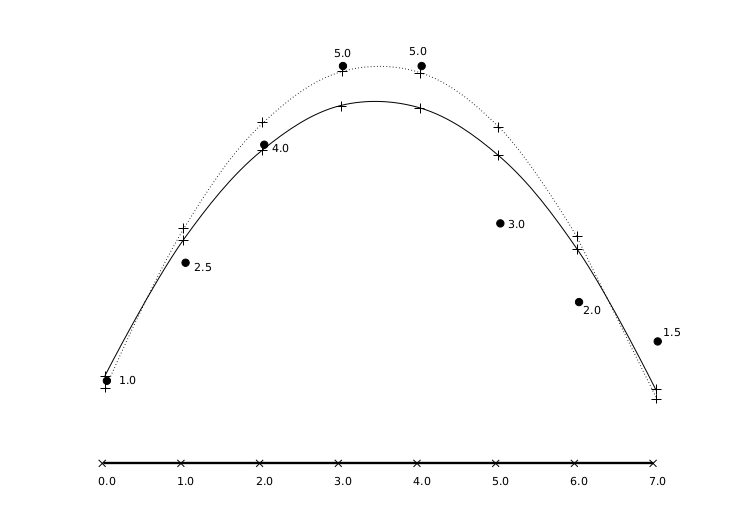
\includegraphics[width=\textwidth]{figures/GLS.png}
	\end{center}
	\caption{Global Least Squares (solid curve) and Weighted Global Least Squares (dashed curve) fit for data represented by the solid circles. The fit is a quadratic fit. The weighting used for the dashed curve is 1.0 every where except at x = 3.0 and x = 4.0 where it is 10.0 (\cite{MLSIntro})}
	\label{fig:gls_example}
\end{figure}
\subsection{Weighted GLS}
\subsection{Weighted Local Least Squares}
\subsection{Moving Least Squares}

\section{Algorithm}
In the Algorithm \ref{alg:mls_alg} general overview of the mls smoothing filter algorithm on MC SDF grid is described. The filter can be applied iteratively, similarly to blur SDF filter. The impact of iterative approach will be described in later section.
\begin{algorithm}[H]
	\scriptsize
	\begin{algorithmic}
		\State generate set of SDF 0-level intersection vertices 
		\State generate neighborClusters form 0-level intersection vertices 
			
		\ForAll{$cluster \in neighborClusters$}
			\State find mls surface approximation for cluster (surfApproximation)
			\ForAll{$vertex \in cluster$}
				\State $newSDF[vertex] \gets newSDF[vertex] + computeUpdatedSDF(vertex, surfApproximation)$
				\State $weights[vertex] \gets weights[vertex] + 1$
			\EndFor
		\EndFor

		\ForAll{$\{vertex, weight\} \in weights$}
			\State $sdfFactor \gets min\left(1, smoothingFactor \cdot \dfrac{fluidParticles[vertex]}{maxFluidParticles}\right)^2$
			\State $newSDF[vertex] \gets sdfFactor \cdot \dfrac{newSDF[vertex]}{weight} + oldSDF[vertex] \cdot (1 - sdfFactor)$
		\EndFor
		\State return levelSet
	\end{algorithmic}
	\caption{mls smoothing filter algorithm}
	\label{alg:mls_alg}
\end{algorithm}
As an input we have an old SDF computed by underlying reconstruction method. From this SDF algorithm detects 0-level intersection vertices (from which final surface vertices will be extracted by linearly interpolating the SDF's between two neighboring vertices with different signs of SDF value). This is required as soon, as the MLS by definition reconstructs surfaces, from SDF that represents a distance to a surface. However, in the used reconstruction methods computed SDF does not represents the distance to a surface along wht whole domain of MC grid. Only the SDF values of 0-level intersection vertices are assumed as a distance to a surface, thus can be used for mls approximation. Intersection cells are shown in the Figure \ref{fig:intersection_vertices}\\
\begin{figure}[H]
	\begin{center}
		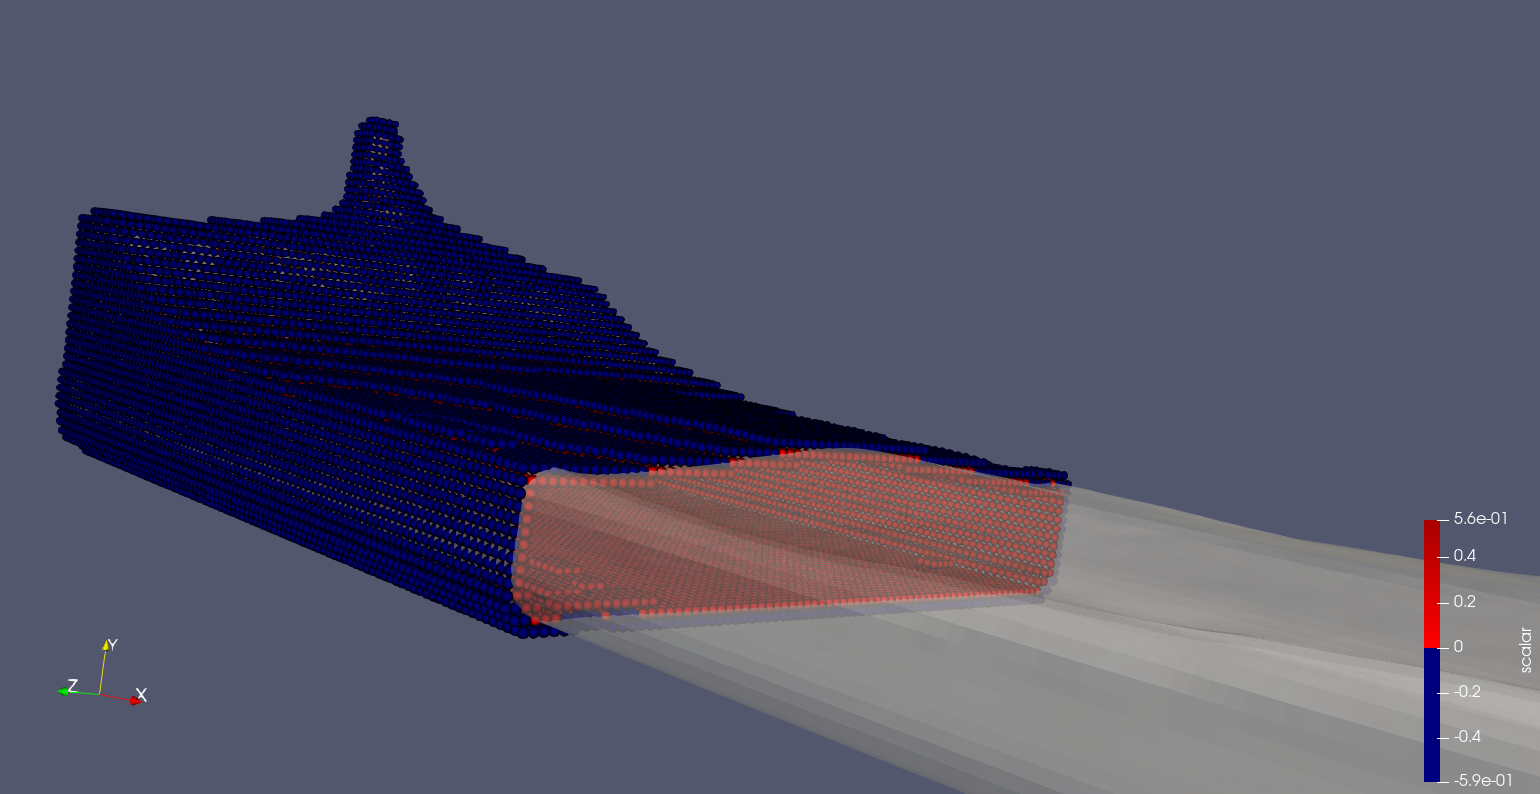
\includegraphics[width=\textwidth]{figures/MlsIntersectionVertexSet.png}
	\end{center}
	\caption{0-level intersection MC grid vertices}
	\label{fig:intersection_vertices}
\end{figure}

Another advantage of using only this set of 0-level intersection vertices is that the algorithm can exactly determine the set of neighbor MC vertices that lie along the reconstructed surface, without approximating the surface normal and taking approximate neighbor set along the tangential direction to the normal. Some computed clusters are represented in the Figure \ref{fig:clusters}\\
\begin{figure}[H]
	\begin{center}
		\begin{subfigure}[b]{0.45\textwidth}
			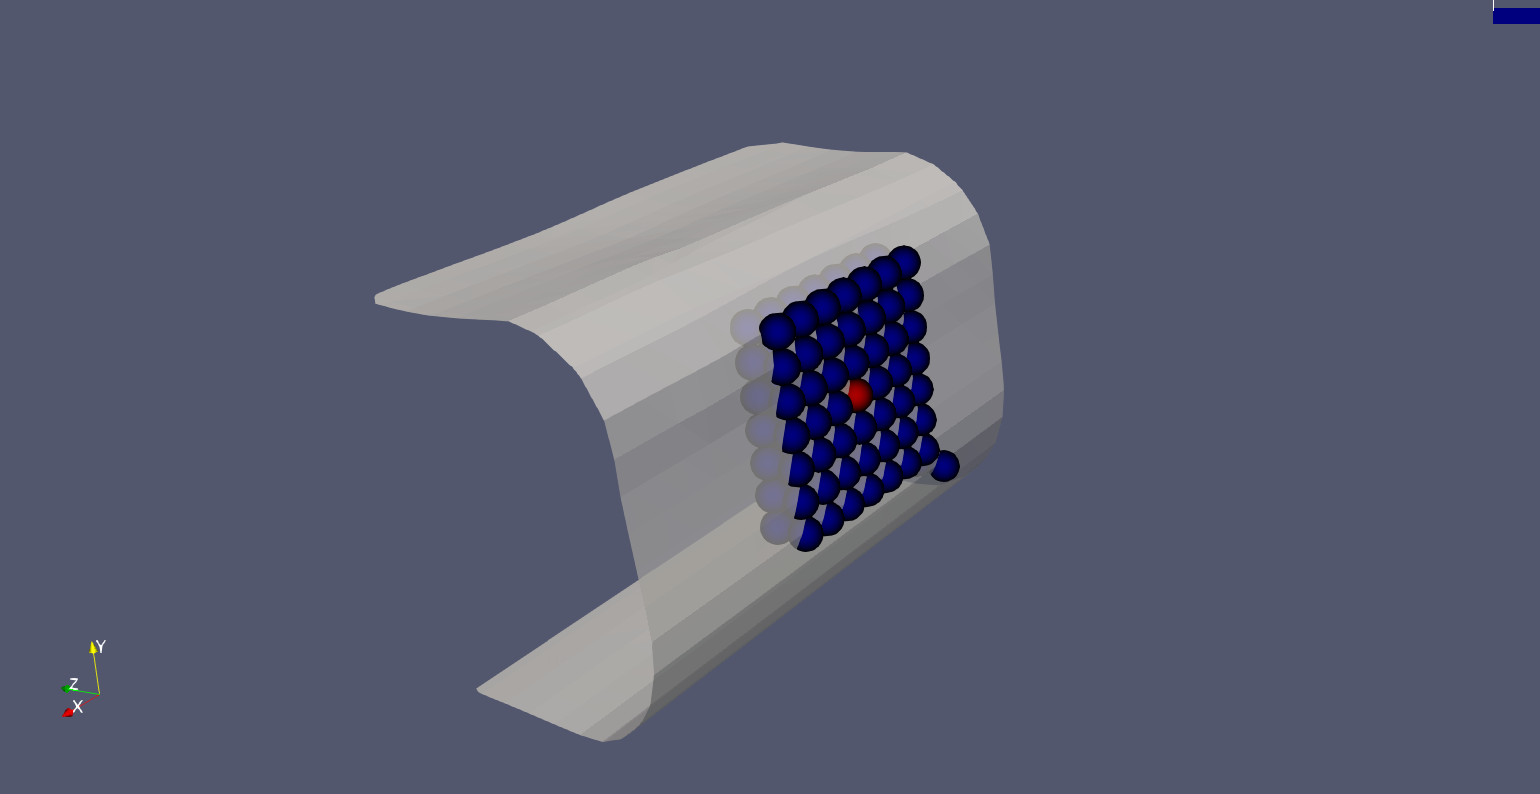
\includegraphics[width=\textwidth]{figures/MlsCluster.png}
		\end{subfigure}
		\begin{subfigure}[b]{0.45\textwidth}
			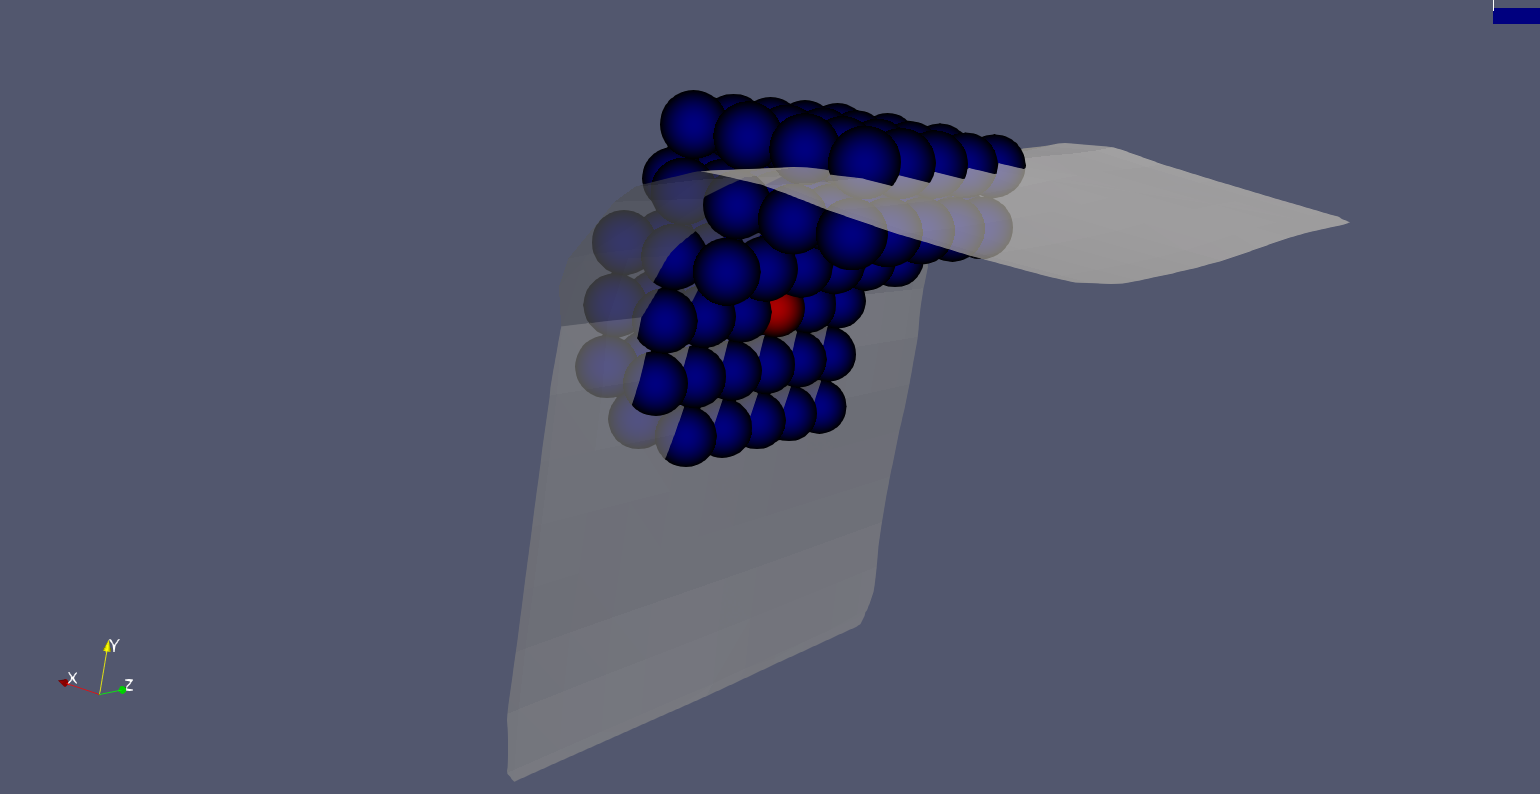
\includegraphics[width=\textwidth]{figures/MlsCluster2.png}
		\end{subfigure}
	\end{center}
	\caption{Examples of computed clusters. Red sphere is a reference vertex, for which cluster is computed.}
	\label{fig:clusters}
\end{figure}

And the last important advantage is a performance influence, as far as there is no need to compute costly mls approximation for MC grid vertices that are not in the SDF 0-level neighborhood.\\

However, there is no guarantee that after the applying approximation the SDF sign of the MC grid vertex will not be switched, e.g. if some MC grid vertex had a positive SDF value before smoothing, after mls approximation it can take a negative value. In this case the set of 0-level intersection vertices set will be changed, and some of the MC grid vertices, that was not mls smoothed will be used during the final surface generation and can bring another noise to the reconstructed surface. This issue can be worked around by applying multiple iteration of mls smoothing trading off final surface smoothness and reconstruction performance.\\

Then clusters are computed, which will be used in the mls approximation. For each cluster coefficients of mls approximated surface is computed, and based on the solution new SDF values are generated for each vertex in the cluster. As soon as vertices can appear in multiple clusters the total values are summed up and then the final value should be divide by a sum of weights. For simplicity and maximization of surface smoothing it was decided to uniformly pick each component of the mls corrected SDF to new corrected SDF from each cluster (all weights of mls corrected sdf values are equal to 1).\\

For thin and small feature areas, where smoothing could bring artifacts, smoothing factor is computed and applied to the final mls value as a weighted sum between the old SDF value and new mls corrected SDF value.\\

\subsection{Clusters computation}
After computing the 0-level intersection vertices of MC grid, clusters are computed. The clusters are a set of neighbor vertices, picked from the 0-level intersection vertices set, which, after all, will be used to compute a mls approximation. The Algorithm \ref{alg:computeClusters} describes the procedure of clusters generation.
\begin{algorithm}[H]
	\scriptsize
	\begin{algorithmic}
			\State $vertices \gets zeroVertexIntersectionCells$
			\While{$vertices$ is not empty}
				\State $vertex \gets vertices.top()$
				\State compute vertex curvature

				\State $maxSamplesFactor \gets \left(\dfrac{min(\dfrac{1}{|curvature|}, fluidParticleDiameter \cdot FluidParticlesCurvatureRadius)}{fluidParticleDiameter \cdot FluidParticlesCurvatureRadius}\right)^2$
				\State $maxSamples \gets MaxSamples \cdot maxSamplesFactor$

				\State $cluster \gets getNeighbourCells(zeroVertexIntersectionCells, vertex, maxSamples)$
				\State add cluster to clusters
			\EndWhile
			\State return clusters
	\end{algorithmic}
	\caption{mls clusters computation}
	\label{alg:computeClusters}
\end{algorithm}
Here $zeroVertexIntersectionCells$ is a previously computed set of MC grid vertices  that are in the neighborhood of the 0-level SDF,  
$fluidParticleDiameter$ is a diameter of a SPH fluid particles, $FluidParticlesCurvatureRadius$ is a number of particles that can fit in a curvature mean radius (user defined), $MaxSamples$ - user defined maximum number of neighbor vertices, that should be put into a single cluster, $SampleOverlapFactor$ - is a [0, 1] factor measure of how much of a neighbor  vertices within current vertex in the cluster should be removed from the $vertices$ set to avoid re-computation of a cluster for them.\\
Before the algorithm iterates over the vertices in the 0-level intersection vertices set, they are duplicated in separate storage($vertices$). This is required to to be able to remove some of the neighbor vertices from the intersection vertex set to avoid re-computation of the clusters for this vertices, in the mean time to use unchanged set of $zeroVertexIntersectionCells$ in the neighborhood search algorithm. This step adds a trade-off between the reconstruction runtime and surface quality. More explanations will be added in next sections.\\
Next the curvature of the current processed vertex is computed. To save a sharp features of the fluid surface it was decided to decrease the number of neighbors in the cluster, for which mls approximation will be applied. Based on the mean curvature of current 0-level intersection vertex number of samples in the cluster is computed. The curvature is computed using the method described in \cite{CurvatureComputation}. firstly compute the curvature for each surface particle that resides in
this cell with the help of its neighboring particles as:
\begin{equation}
	c_i = \sum_j{(1 - n_i \cdot n_j)\cdot k_c(x_i-x_j, h)}
\end{equation}
where $j$ stands for the neighboring particles, $n_i, n_j$ is the normal of any particle and
$k_c$ is the kernel function described as:
\begin{equation}
	k_c(x_i-x_j, h) = max\left(0, \dfrac{1 - |x_i - x_j|}{h}\right)
\end{equation}
Finally, the curvature of any surface cell is approximated as:
\begin{equation}
	c_{cell} = \dfrac{\sum_i{c_i}}{N}
\end{equation}
where i and N represent the surface particles and the total number of surface
particles inside the cell, respectively.\textcolor{red}{TODO: add picture of the computed maxSamplesFactor}

\subsection{MLS neighborhood search}
Neighbors detection is described in pseudo-code of Algorithm \ref{alg:mls_nbsearch}
\begin{algorithm}[H]
	\scriptsize
	\begin{algorithmic}
		\State push $BaseMcVertex$ to $todoMlsVertices$
		\While{$sizeof(neighborCells) < MlsSamples \land todoMlsVertices \ne \emptyset$}
			\State $currentMcVertex \gets todoMlsVertices[0]$
			\State $todoMlsVertices \gets todoMlsVertices \ todoMlsVertices[0]$
			\If{$indexOf(currentMcVertex) \in SelectedIndices \lor SelectedIndices = \emptyset$}
				\State push currentMcVertex back to neighborCells
			\EndIf
			\ForAll{ $nc \in nearest neighbors of currentMcVertex$}
				\If{$nc \in ZeroLevelIntersectionVertices \land nc \not\in neighborCells \land nc \not\in todoMlsVertices$}
					\State push $nc$ back to todoMlsVertices;
				\EndIf
			\EndFor
		\EndWhile
		return neighborCells;
	\end{algorithmic}
	\caption{mls MC vertex neighbors search}
	\label{alg:mls_nbsearch}
\end{algorithm}
As an input algorithm procedure receives a  $BaseMcVertex$ - a MC vertex for which neighborhood is going to be detected, $ZeroLevelIntersectionVertices$ - 0-level intersection MC vertices which was explained above and $SelectedIndices$ - a set of indeces of neighbors, that should be accepted as a samples (more explanations are in the next section). The procedure returns a set of MC grid vertices, that are in the nearest neighborhood within a requested $BaseMcVertex$, and which are in a set of 0-level intersection MC vertices. The output array has important some properties, that will be exploited further. First of all the all detected neighbors are stored in the array. The further the neighbor is from the base cell the higher index it has inside the array. Figure \ref{fig:mls_neighbor_alignment} shows the example of alignment of detected 0-level intersection neighbors.\\
\textcolor{red}{TODO: add image of neighbors displacement in the array}
\subsubsection{MlsSamples}
The final neighborhood is formed as an area of MC vertices along the 0-level iso surface. The higher value is set int the MlsSamples the larger area of samples within the requested base sample will be configured and the more smoothing will be applied to the SDF, e.g. some examples of computed neighborhood area depending on a number of MlsSamples and respective reconstructed surface are shown in the figure \ref{fig:mls_sample_areas} and figure \ref{fig:mls_samples_example_surfaces}.
\textcolor{red}{TODO: add figures}
Thus modifying number of mls samples influences the final surface quality, in the meantime it increases computation time of the reconstruction.
\subsubsection{SelectedIndices}
To receive a smooth surface it is required to use a large amount of mls samples in the neighborhood as was already shown in previous section. However, it requires much more computation efforts, to compute approximated mls surface and to correct SDF of 0-level vertices. Thus to reduce computation approach it was decided to apply MonteCarlo approach to pick a subset of samples, that was computed by mls neighborhood search, which uniformly represents initially computed set. The hope is that we will be able to correctly detect a our distribution so that the final surface quality will not be degraded too much and the computation time of the reconstruction phase will be reduced.\\
The first idea that comes to mind is just uniformly pick $n$ samples from the computed mls sample buffer. But in this case we need to uniformly pick samples from each distance from the central sample. The probability of picking samples far away from the base sample is larger then the probability of picking the samples near the base cell, e.g. taking for simplicity circle will be used to show  the probability distribution. Thus the density  function of picking arbitrary point, that lies in radius $r$ from the current point is shown in equation \ref{eq:probability_distr}.
\begin{equation}
	p(r) = \dfrac{2 \cdot \pi r}{\pi \cdot R^2} = \dfrac{2 \cdot r}{\cdot R^2}
	\label{eq:probability_distr}
\end{equation}
where $R$ is a radius to the sphere. In another words talking the probability of picking sample on that lies from the central sample in a distance of $r$ is equal to length of the inner circle with radius $r$ divided by the area of the sphere.
Thus to pick samples from the buffer uniformly w.r.t. the distance from the central sample we have to modify the probability distribution of picking a samples from buffer. Next procedure is applied to pick the sample indeces from the buffer:
\begin{algorithm}[H]
	\scriptsize
	\begin{algorithmic}
			\State $acceptedIndices \gets \{0\}$;
			\State $lowerBound \gets 0$
			\State $upperBound \gets (MlsSamples - 1)$
			\For{$i \in [0, MaxSamples]$}
				\State $offset \gets \dfrac{PickRandom(0, MaxSamples - 1)}{MaxSamples}$
				\State $index \gets lowerBound + offset^2 \cdot (upperBound - lowerBound))$
				\State $currentIndex \gets index$
				\While{$index \in acceptedIndices$}
					\If{$index = lowerBound$}
						\State $index = upperBound$
					\Else
						\State $index \gets index - 1$
					\EndIf
				\EndWhile
				\State $acceptedIndices \gets acceptedIndices \cup index$;
				\If{$index = lowerBound$}
					\State $index++;$
					\While{$index \in acceptedIndices$}
						\State $index++$
					\EndWhile
					\State $lowerBound \gets index$
				\Else 
					\If{$index = upperBound$}
						\State $index--;$
						\While{$index \in acceptedIndices$}
							\State $index--$
						\EndWhile
						\State $upperBound \gets currentIndex$
					\EndIf
				\EndIf
			\EndFor
	\end{algorithmic}
	\caption{random sampling of indices's in the mls neighborhood}
	\label{alg:mls_montecarlo_sampling}
\end{algorithm}
The idea of the algorithm is to generate set of indexes from domain of mls neighborhood buffer, and after that shift the index to the beginning. This way the probability distribution of picking sample from specific distance from the center of the area will be compensated and converge to uniform distribution. Figure \ref{fig:distributions} shows the distributions of sampling indexes before quadratic shifting (uniformly pick the index of the buffer) and after (pick index uniformly and shift it according to the $x^2$ function).\\
\begin{figure}
	\begin{tikzpicture}
		\begin{axis}
			[
				xlabel={$x$},
				ylabel={$y$},
				ymin = 0,
				ymax = 0.1,
				width = 0.45\textwidth
			]
			\addplot[
				red,
				mark=*
			] table{initialDistributionOverLevels.txt};
		\end{axis}

	\end{tikzpicture}
	\begin{tikzpicture}
		\begin{axis}
			[
				xlabel={$x$},
				ylabel={$y$},
				ymin = 0,
				ymax = 0.1,
				width = 0.45\textwidth
			]
			\addplot[
				blue,
				mark=*
			] table{resultingDistributionOverLevels.txt};
		\end{axis}
	\end{tikzpicture}
	\caption{Initial distribution of the samples over area levels (left) and final distribution after modifying indexes (right)}
	\label{fig:distributions}
\end{figure}
where $x$ is a probability of picking sample on level $i$ from the center of area, $y$ - is a depth of the level. The distributions where generated empirically by sampling 10000 indices's over the whole domain of the buffer. Figure \ref{fig:cluster_sampled} shows the cluster, with different sampling types.
\begin{figure}[H]
	\begin{center}
		\begin{subfigure}[b]{0.9\textwidth}
			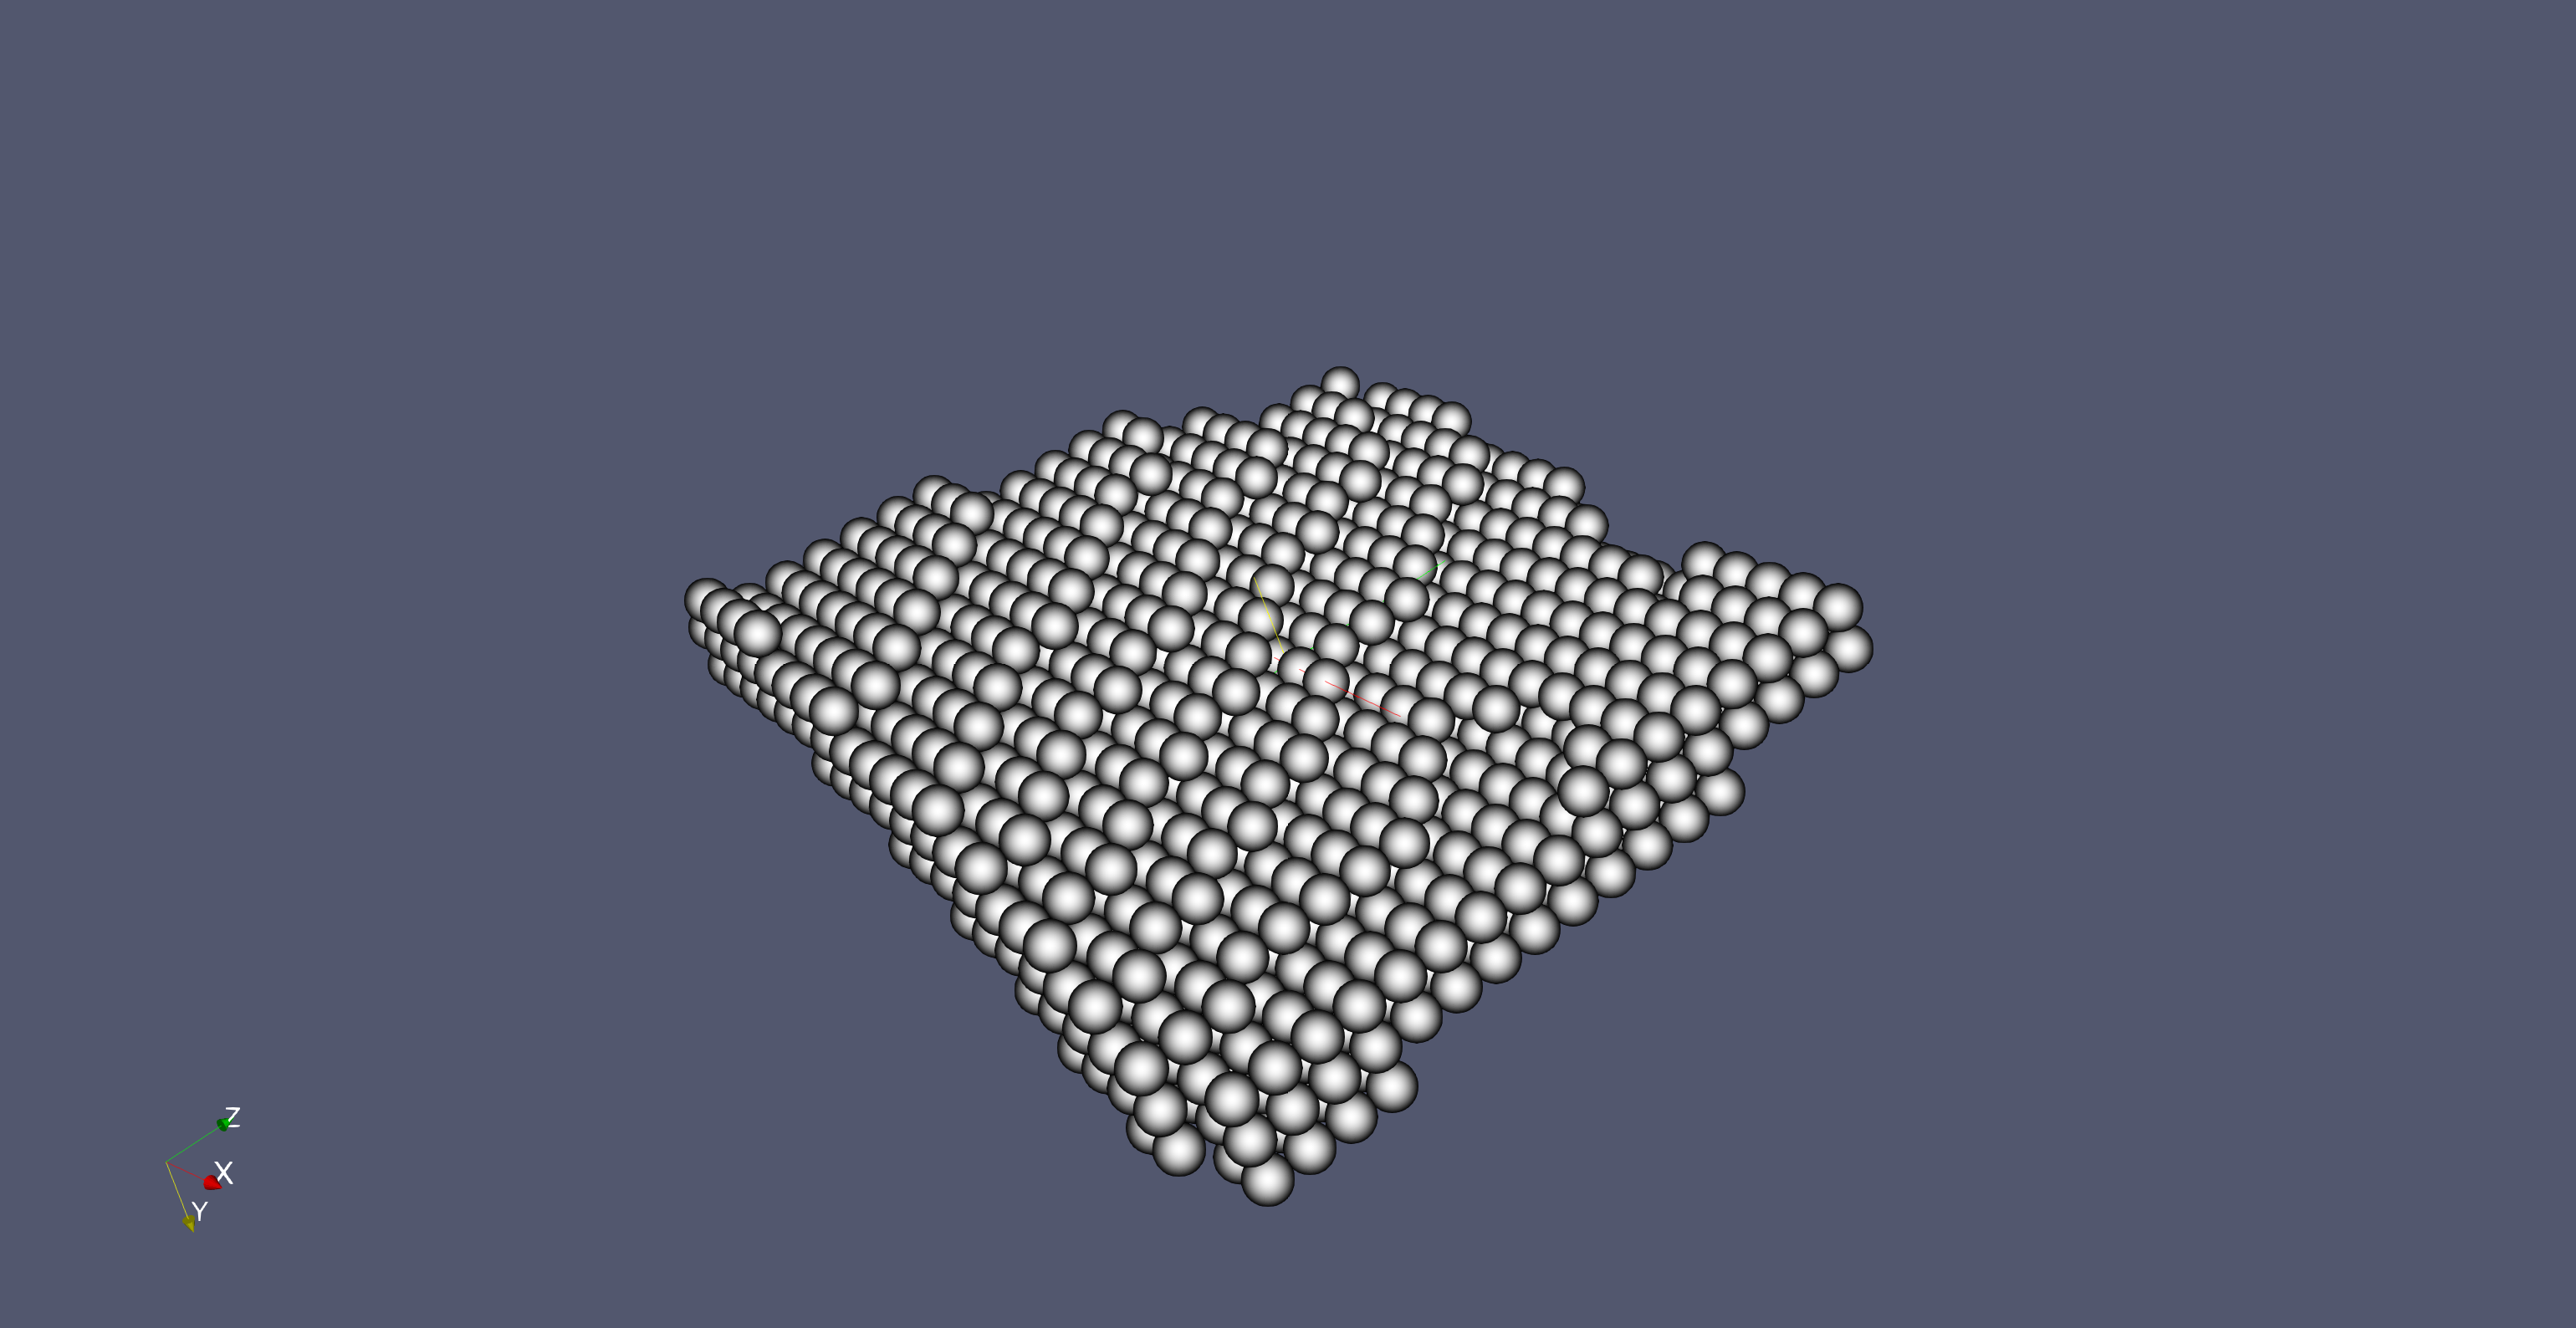
\includegraphics[width=\textwidth]{figures/SamplingFullDomain.png}
			\caption{full set of neighbors}
		\end{subfigure}
		\begin{subfigure}[b]{0.9\textwidth}
			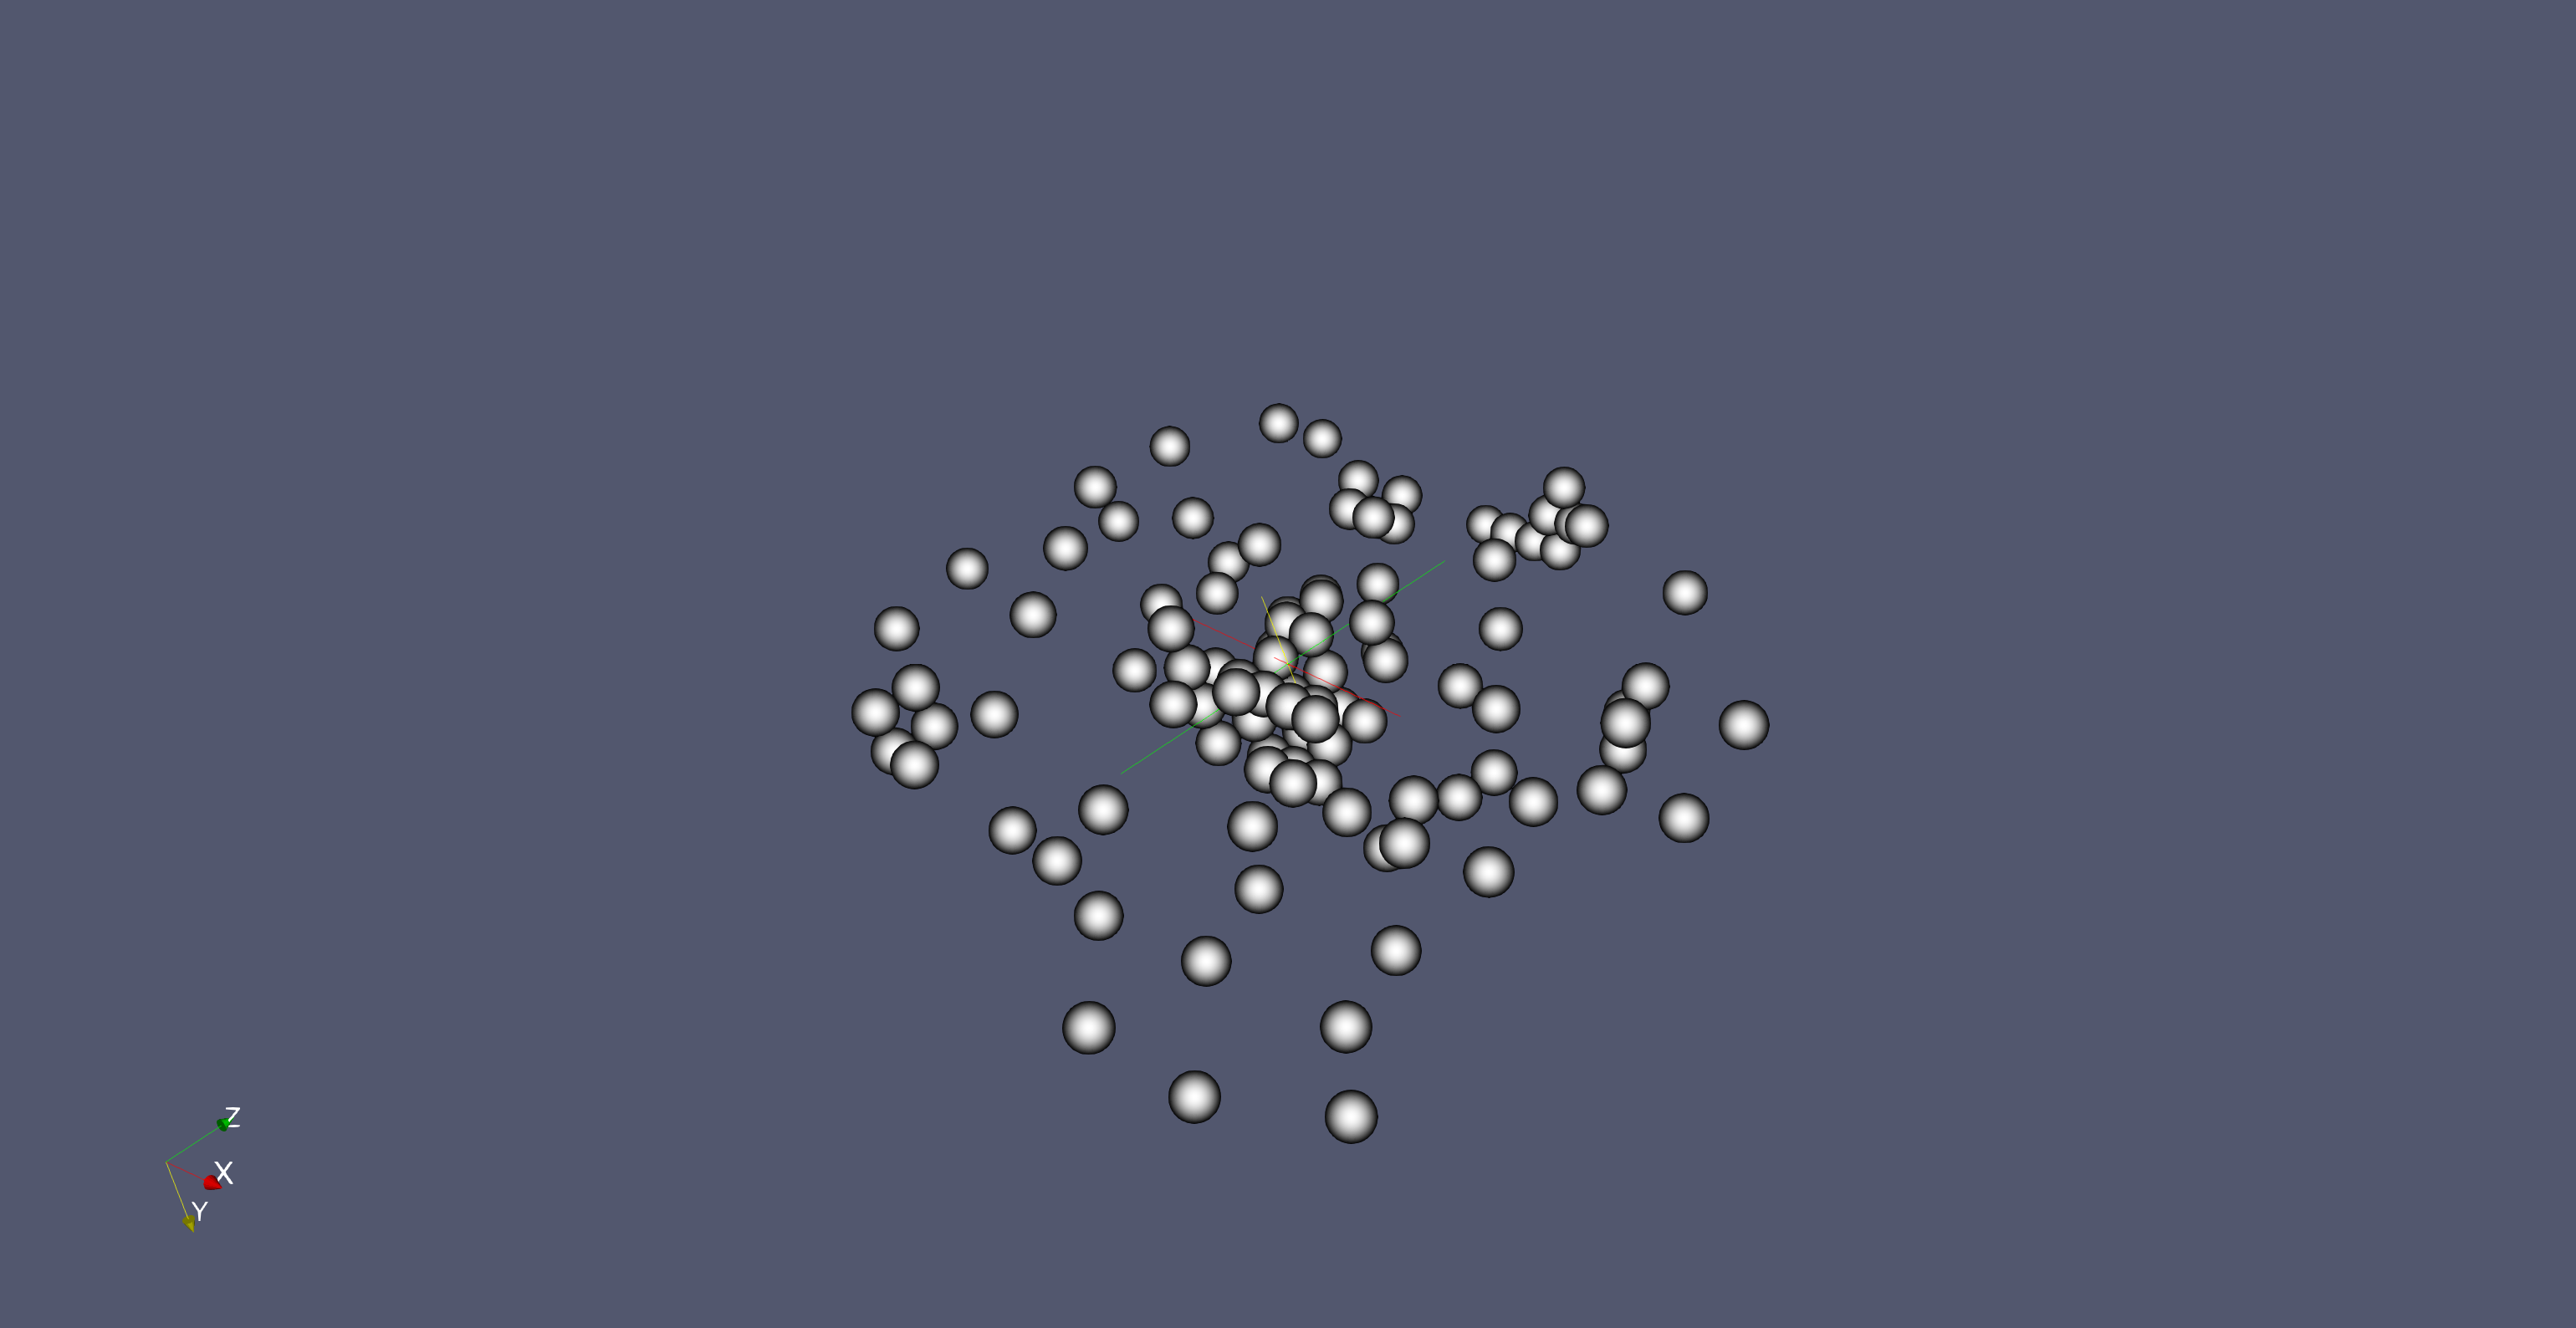
\includegraphics[width=\textwidth]{figures/SamplingQuadratic.png}
			\caption{set of samples with quadratic shift}
		\end{subfigure}
		\begin{subfigure}[b]{0.9\textwidth}
			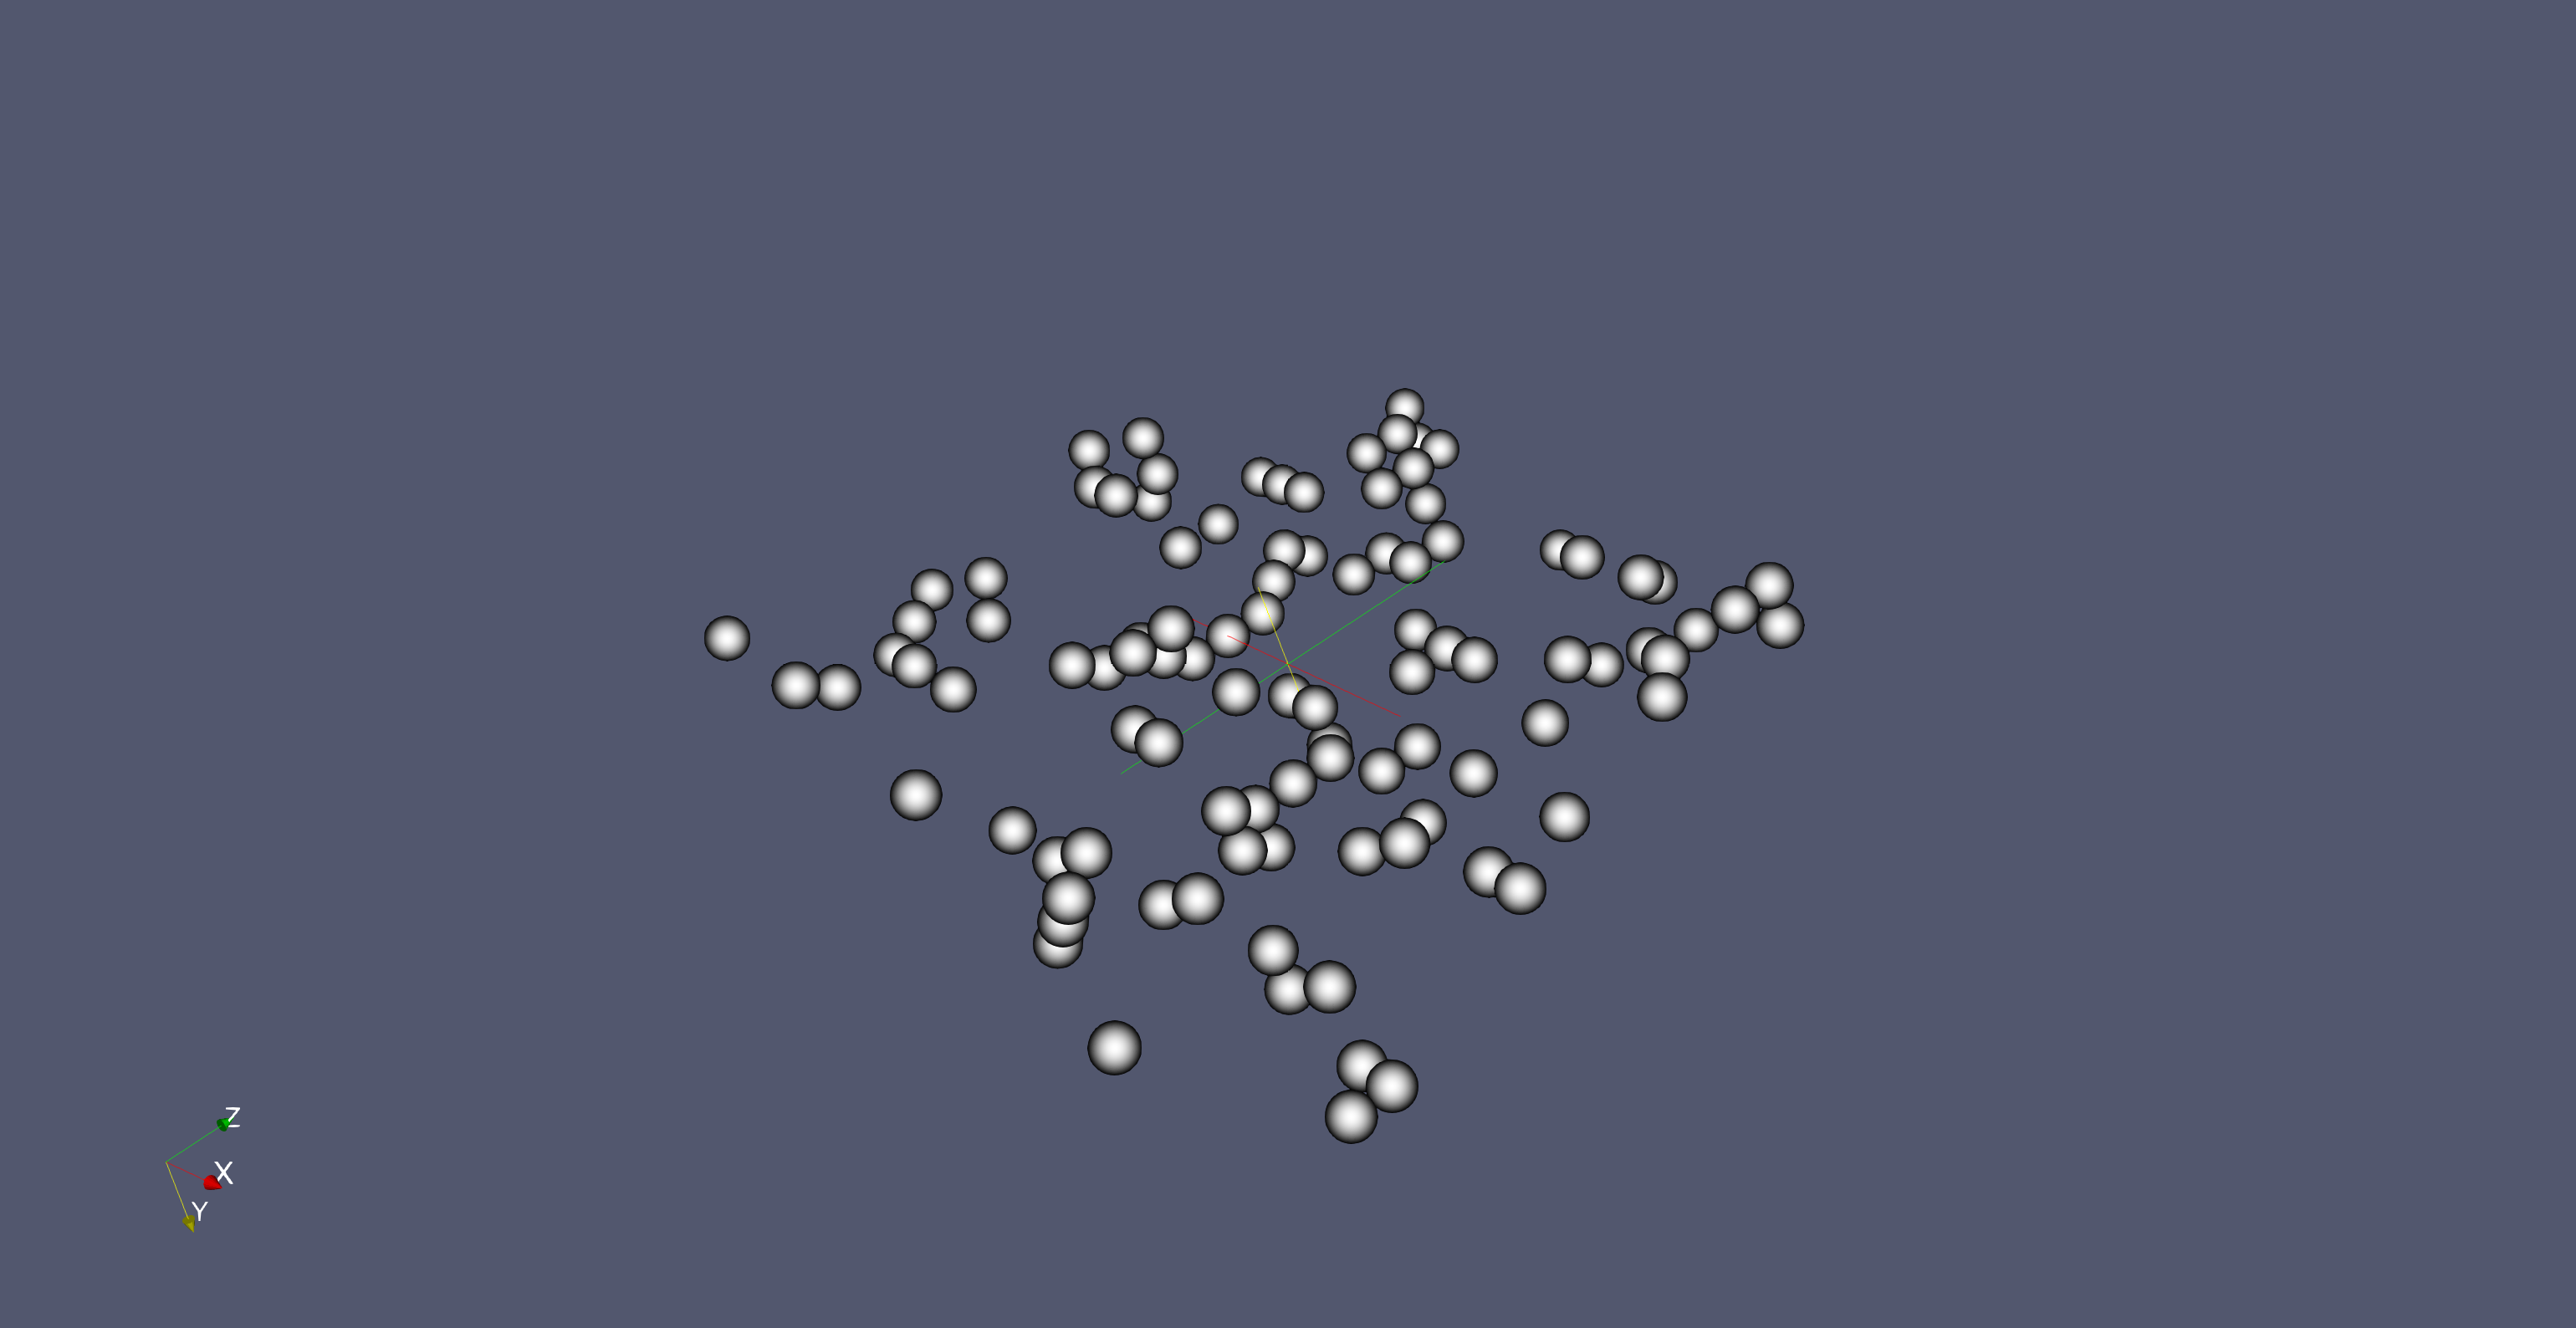
\includegraphics[width=\textwidth]{figures/SamplingUniform.png}
			\caption{uniformly sampled set}
		\end{subfigure}
	\end{center}
	\caption{sampling of mls neighbor vertices set} \label{fig:cluster_sampled}
\end{figure}
In the quadratic shift sampling approach most of the samples are concentrated in the center of the cluster, thus compensating the number of samples, that are far away from the center and that are near to the center. In the uniform approach samples are spreader along the area.\\
In Figure \ref{fig:surface_sampling_results} some examples of influence using sampled subset of the full set of particles is shown.
\begin{figure}[H]
	\begin{center}
		\begin{subfigure}[b]{\textwidth}
			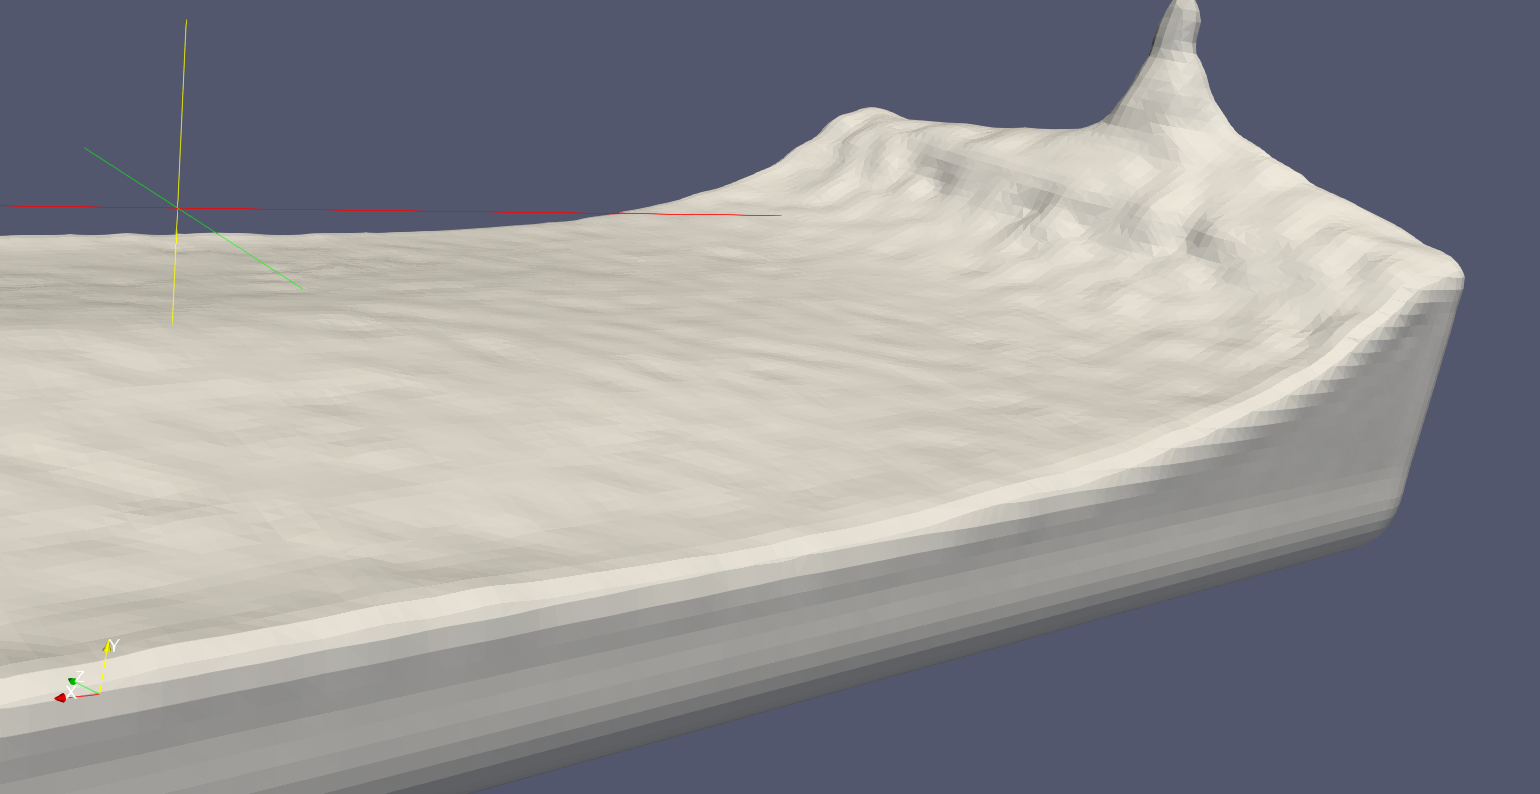
\includegraphics[width=\textwidth]{figures/MLSSurfaceOriginal.png}
			\caption{original surface}
		\end{subfigure}
		\begin{subfigure}[b]{\textwidth}
			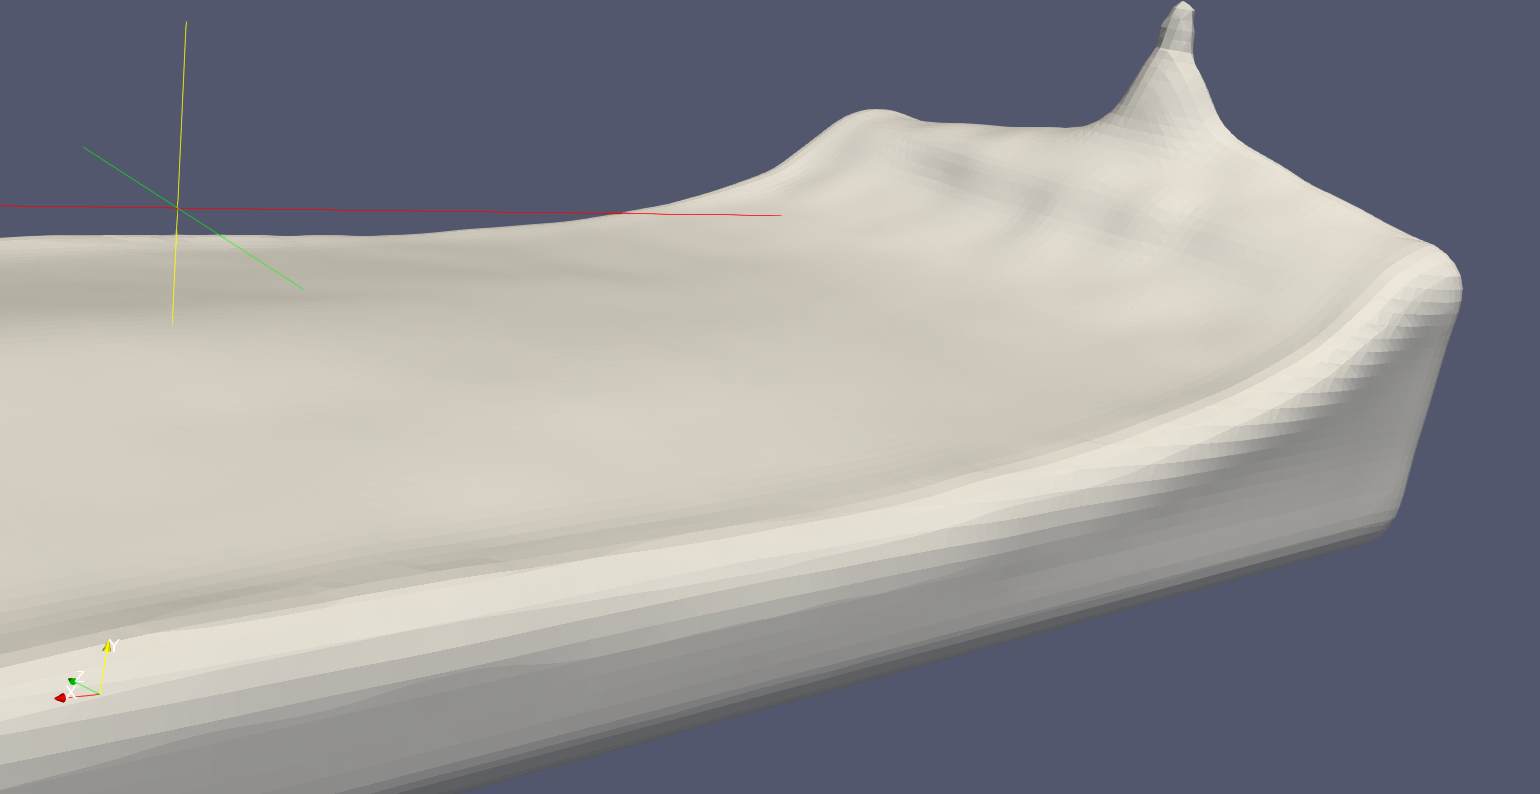
\includegraphics[width=\textwidth]{figures/MLSSurfaceSamplingFullSet.png}
			\caption{mls corrected surface with full set of samples}
		\end{subfigure}
		\begin{subfigure}[b]{\textwidth}
			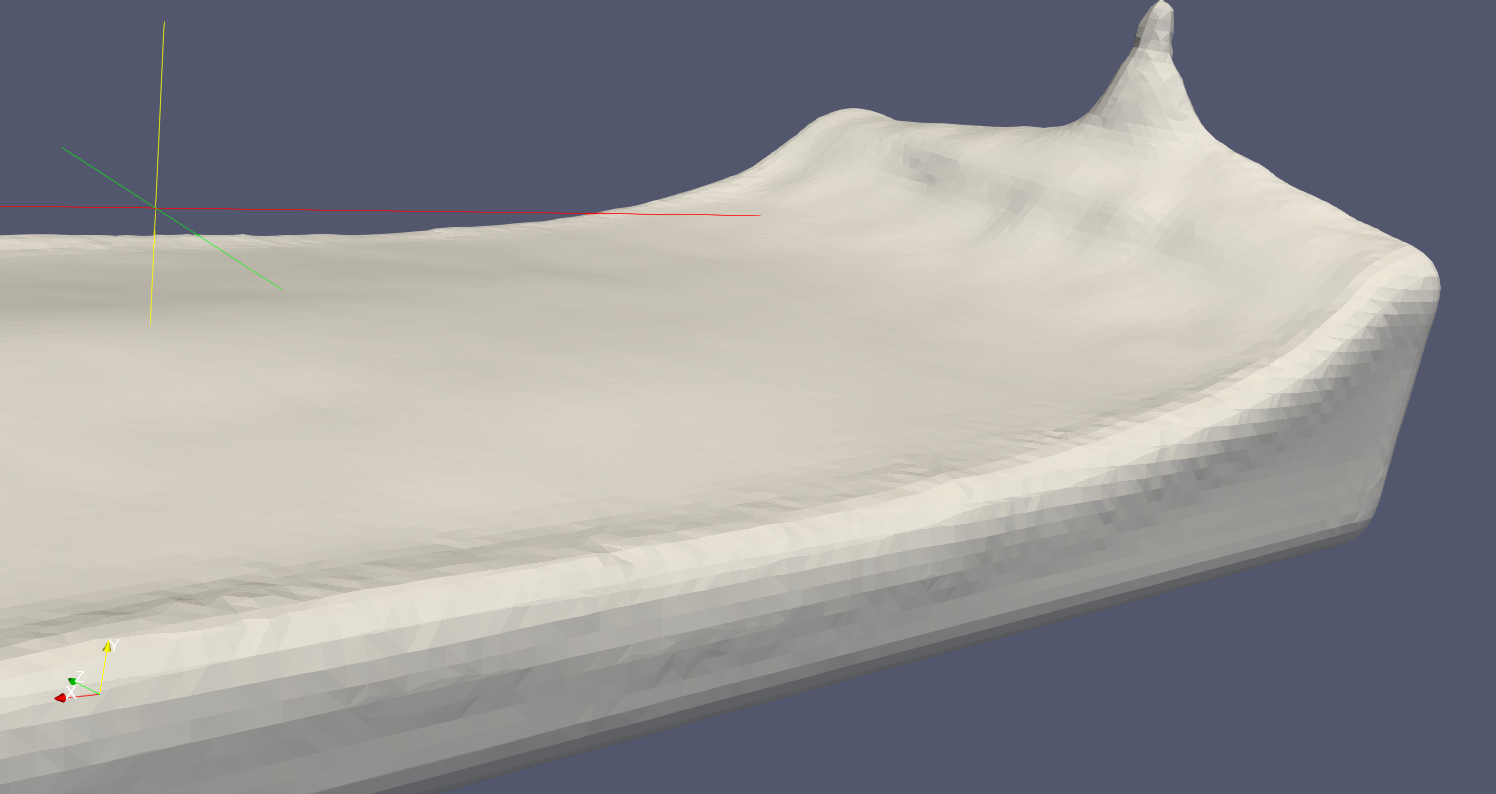
\includegraphics[width=\textwidth]{figures/MLSSurfaceSamplingQuarterSet.png}
			\caption{mls corrected surface with quarter set of samples}
		\end{subfigure}
	\end{center}
	\caption{Reconstructed mls surface} \label{fig:surface_sampling_results}
\end{figure}
Both, full samples set and partial samples set removes bumps from the original surface, but for the reconstruction with $\dfrac{1}{4}$ set of mls samples small frequency noise can be seen on the corner areas.

\subsection{Mls surface computation}

The core of the smoothing method is a computation of an approximated surface. 
The main idea of computational approach was taken from the work of Guennebaud \& Gross \cite{Apss}. 
Given a set of points $P = \{p_i \in R_d \}$, a smooth surface $S_P$ approximating $P$ using a moving least squares spherical fit to the data can be defined. However, in case of this study there is no set of points, that define surface and which should be approximated. As an input we receive a set of points, that are resided near the surface - e.g. the MC grid vertices, that are resided in the nearest neighborhood to the 0-level iso-surface. 
Although, with the MC grid vertices we also have a values of the SDF, which theoretically define the distance to the surface. But in most cases the computed SDF doesn't represent an actual distance to the surface, but just an approximation of the distance, which is more approximate in the neighborhood of the 0-level iso-surface, but is not define the distance to the surface in the further areas of the fluid. 
However, in the 0-level intersection areas SDF also doesn't exactly defines a distance to the surface, which is one of the reason of the occurrence of small frequency bubs on the reconstructed fluid surface. Thus applying mls approximation to the 0-level intersection MC vertices and correcting their SDF is an attempt to reconstruct a smooth distance based SDF.\\
In the APSS work analytical equation of the sphere was used as a core function, that is approximated by applying least squares approximation to a samples set. Given a point $x$ the equation, that represents a distance to the sphere center can be represented as a function of x:
\begin{equation}
f(x) = s_1\cdot x^2 + s_2 \cdot x_x + s_3 \cdot x_y + s_4 \cdot x_z + s_5
\end{equation}
where $x^2$ is a dot product of point $x$ on itself, $s_i$ are unknown coefficients, that are going to be calculated. Thus the goal is to calculate the unknown coefficients $s_i$, and based to the approximated mls surface correct the sdf value by multiplying the MC grid vertex world coordinate by the coefficients:
\begin{equation}
SDF_{new}(x_i) = f(x_i) = s_1\cdot x_i^2 + s_2 \cdot x_{i_x} + s_3 \cdot x_{i_y} + s_4 \cdot x_{i_z} + s_5
\end{equation}
In the Algorithm \ref{alg:mls_alg} each MC grid vertex in the cluster $SDF_{new}$ is computed. As soon as each particle can appear in the cluster multiple times for each cluster, for which mls corrected surface is computed. Then the final SDF is a weighted sum of all sdf's, computed according to the Algorithm \ref{alg:mls_alg}, divided by total sum of weights:
\begin{equation}
	SDF_{mls}(x) = \dfrac{\sum_{j \in Clusters}{SDF_{new_j}(x)}}{|Clusters|}
\end{equation}
where $Clusters$ is a set of clusters, such that $: \forall cluster \in Clusters: x \in cluster$. 
\subsection{Applying mls filter iteratively}
In the Algorithm \ref{alg:mls_alg} it is stated that only computed 0-level intersection MC grid vertices are under the mls correction procedure. In the meantime the MC grid vertices, that are not taking part in surface mesh generation while cells no neighbor vertices contains SDF value transfer from positive to negative and vice-verse, thus the SDF correction procedure is not applied to this vertices. In this case next problem can arise: the corrected MC vertices can change the sign of SDF and will be no more in a subset of the 0-level intersection MC grid vertices, and non corrected vertices, that are in the neighborhood of the stated vertices, will not take part in surface generation. In the Figure \ref{fig:mls_iterations} shown the effect of applying mls correction on the 0-level intersection MC grid vertices:
\begin{figure}[H]
	\begin{center}
		\begin{subfigure}[b]{0.9\textwidth}
			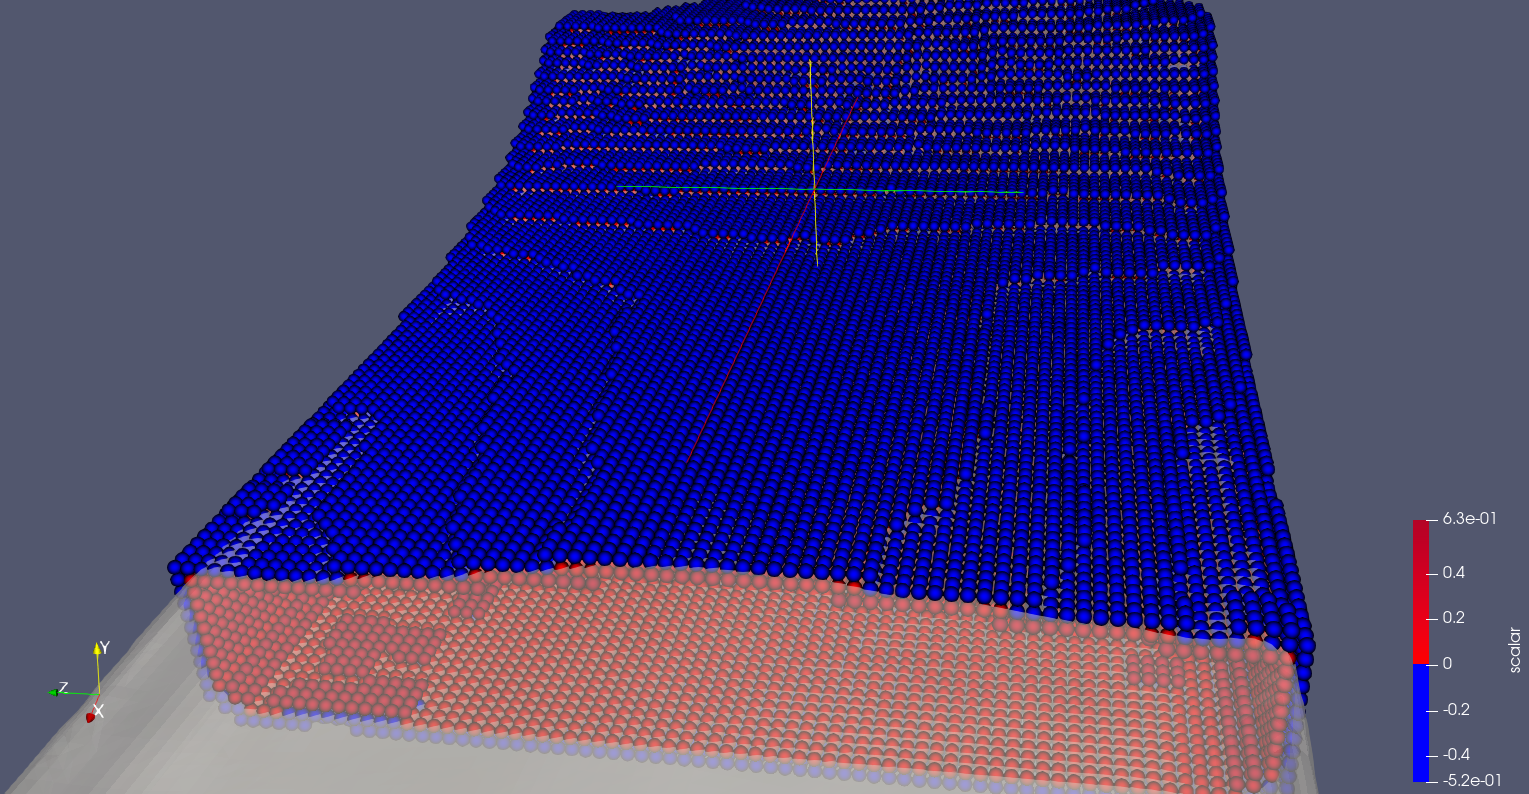
\includegraphics[width=\textwidth]{figures/IntersectionCellsSdfBeforeMls_1_iter.png}	
			\caption{Before mls smoothing} \label{fig:mls_0_iter}
		\end{subfigure}
		\begin{subfigure}[b]{0.9\textwidth}
			\includegraphics[width=\textwidth]{ figures/IntersectionCellsSdfAfterMls_1_iter.png}	
			\caption{1 iterations of mls smoothing} \label{fig:mls_1_iter}
		\end{subfigure}
		\begin{subfigure}[b]{0.9\textwidth}
			\includegraphics[width=\textwidth]{figures/IntersectionCellsSdfAfterMls_3_iter.png}	
			\caption{3 iterations of mls smoothing} \label{fig:mls_3_iter}
		\end{subfigure}
	\end{center}
	\caption{Subset of 0-level intersection MC grid vertices with SDF values before and after mls smoothing. Red are vertices with positive SDF valuations, blue are vertices with negative SDF value.} 
	\label{fig:mls_iterations}
\end{figure}
After application of mls it can be seen on the picture, that some MC grid vertices changed its SDF sign from negative to positive (Figure \ref{fig:mls_1_iter}). After 3 iterations of mls filter smoothing the effect of SDF sign switch is applied to smaller subset of MC grid vertices (Figure \ref{fig:mls_3_iter}). This can be explained by the convergence of the surface to some invariant state, since each iteration the average standard deviation of SDF values before and after the application of MLS among all clusters gradually decreases and converges to 0:
\begin{figure}[H]
	\begin{center}
		\begin{tikzpicture}
			\begin{axis}
				[
					xlabel={$x$},
					ylabel={$y$},
					width = 0.45\textwidth
				]
				\addplot[
					red,
					mark=*
				] table{mls_std_dev.txt};
			\end{axis}
		\end{tikzpicture}
	\end{center}
	\caption{Standard deviation from initial SDF value to mls corrected (average among all clusters)}
	\label{fig:mls_std_dev}
\end{figure}
There are some examples of reconstructed surface shown in the Figure \ref{fig:mls_surf_iter_examples} given different amount of iterations.
\begin{figure}[H]
	\begin{center}
		\begin{subfigure}[b]{0.47\textwidth}
			\includegraphics[width=\textwidth]{figures/MlsSurfaceInitial.png}
			\caption{original surface}
		\end{subfigure}
		\begin{subfigure}[b]{0.47\textwidth}
			\includegraphics[width=\textwidth]{figures/MlsSurface1Iteration.png}
			\caption{Mls correction 1 iteration}
		\end{subfigure}
		\begin{subfigure}[b]{0.47\textwidth}
			\includegraphics[width=\textwidth]{figures/MlsSurface2Iteration.png}
			\caption{Mls correction 2 iterations}
		\end{subfigure}
		\begin{subfigure}[b]{0.47\textwidth}
			\includegraphics[width=\textwidth]{figures/MlsSurface3Iteration.png}
			\caption{Mls correction 3 iterations}
		\end{subfigure}
		\begin{subfigure}[b]{0.47\textwidth}
			\includegraphics[width=\textwidth]{figures/MlsSurface4Iteration.png}
			\caption{Mls correction 4 iterations}
		\end{subfigure}
		\begin{subfigure}[b]{0.47\textwidth}
			\includegraphics[width=\textwidth]{figures/MlsSurface5Iteration.png}
			\caption{Mls correction 5 iterations}
		\end{subfigure}
	\end{center}
	\caption{Reconstructed mls surface} \label{fig:mls_surf_iter_examples}
\end{figure}
\begin{figure}[H]
	\begin{center}
		\begin{subfigure}[b]{0.47\textwidth}
			\includegraphics[width=\textwidth]{figures/MLS2SurfaceOriginal.png}
			\caption{original surface}
		\end{subfigure}
		\begin{subfigure}[b]{0.47\textwidth}
			\includegraphics[width=\textwidth]{figures/Mls2Surface1Iteration.png}
			\caption{Mls correction 1 iteration}
		\end{subfigure}
		\begin{subfigure}[b]{0.47\textwidth}
			\includegraphics[width=\textwidth]{figures/Mls2Surface2Iteration.png}
			\caption{Mls correction 2 iterations}
		\end{subfigure}
		\begin{subfigure}[b]{0.47\textwidth}
			\includegraphics[width=\textwidth]{figures/Mls2Surface3Iteration.png}
			\caption{Mls correction 3 iterations}
		\end{subfigure}
		\begin{subfigure}[b]{0.47\textwidth}
			\includegraphics[width=\textwidth]{figures/Mls2Surface4Iteration.png}
			\caption{Mls correction 4 iterations}
		\end{subfigure}
		\begin{subfigure}[b]{0.47\textwidth}
			\includegraphics[width=\textwidth]{figures/Mls2Surface5Iteration.png}
			\caption{Mls correction 5 iterations}
		\end{subfigure}
	\end{center}
	\caption{Reconstructed mls surface} \label{fig:mls_surf_iter_examples}
\end{figure}

The more iterations are applied for the mls correction the smoother surface we receive. However, according to the figure \ref{fig:mls_surf_iter_examples} large amount of iteration destroys tiny fluid features, such as splashes, or shrinks fluid surface in thin areas. This can be controlled via the smoothing factor calibration, but for the purpose of this thesis, removal of small frequency bumps on the reconstructed surface, one iteration is enough in most cases.

\section{Performance analysis}
\section{Results}
\section{Conclusions}
\begin{appendices}
\input{appendix.tex}
\end{appendices}
\cleardoublepage

\backmatter
\phantomsection
\addcontentsline{toc}{chapter}{Bibliography}
\begingroup
\setlength{\emergencystretch}{8em}
\printbibliography{}
\endgroup

\cleardoublepage
\phantomsection
\addcontentsline{toc}{chapter}{Index}
\printindex
\cleardoublepage

\end{document}
